\section{บทที่ 3 แบบจำลองทางคณิตศาสตร์และฟังก์ชันถ่ายโอน}

%\textbf{ชื่อบทภาษาอังกฤษ:} Mathematical Modeling and Transfer Function\\\textbf{รายวิชา:} ระบบควบคุม\\\textbf{รหัสวิชา:} ไม่ระบุ\\\textbf{จำนวนหน่วยกิต:} ไม่ระบุ\\\textbf{ระดับผู้เรียน:} นักศึกษาปริญญาตรี\\\textbf{เวลาสอน:} บรรยาย 6 ชั่วโมง และกิจกรรมปฏิบัติการบูรณาการตามความพร้อมของรายวิชา\\\textbf{ความยาวเป้าหมาย:} 25–30 หน้า A4 สำหรับเนื้อหาหลัก โดยไม่นับภาคผนวกเฉลยละเอียด\\\textbf{รูปแบบการเรียน:} บรรยายร่วมกับการคำนวณ การจำลอง และกิจกรรมปฏิบัติการ\\\textbf{โหมดการออกแบบ:} Topic-Based Design Mode

%\begin{quote}
%\textbf{จุดเน้นของบท:} การแปลงระบบจริงเป็นสมการเชิงอนุพันธ์ และแปลงสมการเชิงอนุพันธ์เป็นฟังก์ชันถ่ายโอนในโดเมนเชิงซ้อนหรือโดเมน $s$
%\end{quote}

%\par\noindent\rule{\textwidth}{0.4pt}\par

\subsection{1. แนวคิดสำคัญของบท}

ระบบควบคุมทางวิศวกรรมประกอบด้วยอุปกรณ์จริงที่มีพฤติกรรมเปลี่ยนแปลงตามเวลา เช่น ตำแหน่งของมวล ความเร็วของมอเตอร์ แรงดันไฟฟ้าของตัวเก็บประจุ หรืออุณหภูมิของกระบวนการ การวิเคราะห์ระบบเหล่านี้โดยพิจารณาเฉพาะโครงสร้างทางกายภาพมักทำได้ยาก จึงต้องสร้าง \textbf{แบบจำลองทางคณิตศาสตร์ (Mathematical Model)} เพื่อแทนความสัมพันธ์ระหว่างอินพุต เอาต์พุต และตัวแปรภายในของระบบ

กระบวนการสร้างแบบจำลองเริ่มจากการกำหนดขอบเขตระบบ เลือกอินพุตและเอาต์พุต ตั้งสมมติฐาน และใช้กฎทางฟิสิกส์สร้างสมการเชิงอนุพันธ์ จากนั้นใช้การแปลงลาปลาซเพื่อเปลี่ยนสมการในโดเมนเวลาเป็นสมการพีชคณิตในโดเมน $s$ ภายใต้เงื่อนไขค่าเริ่มต้นเป็นศูนย์ อัตราส่วนระหว่างการแปลงลาปลาซของเอาต์พุตกับอินพุตเรียกว่า \textbf{ฟังก์ชันถ่ายโอน (Transfer Function)}

ฟังก์ชันถ่ายโอนช่วยให้ผู้เรียนสามารถเปรียบเทียบระบบต่างชนิดด้วยรูปแบบทางคณิตศาสตร์เดียวกัน วิเคราะห์อันดับของระบบ โพล ซีโร อัตราขยาย และเชื่อมโยงไปสู่การวิเคราะห์การตอบสนอง เสถียรภาพ และการออกแบบตัวควบคุมในบทถัดไป อย่างไรก็ตาม ฟังก์ชันถ่ายโอนแสดงความสัมพันธ์อินพุต–เอาต์พุตเป็นหลัก จึงไม่อธิบายสถานะภายในทั้งหมดของระบบ การเขียนสมการสถานะจึงเป็นอีกแนวทางที่ช่วยเก็บข้อมูลตัวแปรภายในและรองรับระบบหลายอินพุตหลายเอาต์พุตได้ดีกว่า

\par\noindent\rule{\textwidth}{0.4pt}\par

\subsection{2. ความรู้พื้นฐานก่อนเรียน}

ผู้เรียนควรมีความรู้และทักษะต่อไปนี้

\begin{enumerate}
    \item การหาอนุพันธ์และการแก้สมการเชิงอนุพันธ์สามัญเบื้องต้น
    \item การแปลงลาปลาซและสมบัติของอนุพันธ์ในโดเมน $s$
    \item กฎการเคลื่อนที่ข้อที่สองของนิวตัน
    \item กฎแรงดันและกฎกระแสของเคอร์ชอฟฟ์
    \item ความสัมพันธ์ของตัวต้านทาน ตัวเหนี่ยวนำ และตัวเก็บประจุ
    \item หลักการพื้นฐานของวงจรขยายเชิงปฏิบัติการภายใต้แบบจำลองอุดมคติ
    \item การจัดรูปพหุนาม เมทริกซ์ และระบบสมการเชิงเส้น
    \item การใช้เครื่องกำเนิดสัญญาณและออสซิลโลสโคปเบื้องต้นภายใต้แรงดันต่ำ
\end{enumerate}

\par\noindent\rule{\textwidth}{0.4pt}\par

ื\newpage

\subsection{3. คำสำคัญประจำบท}

\begin{table}[htbp]
    \centering
    \begin{tabular}{l l l}
        \hline
        \textbf{คำศัพท์ภาษาไทย} & \textbf{คำศัพท์ภาษาอังกฤษ} & \textbf{ความหมายโดยย่อ} \\
        \hline
        แบบจำลองทางคณิตศาสตร์ & Mathematical Model & สมการหรือความสัมพันธ์ที่ใช้แทนพฤติกรรมของระบบจริง \\
        ระบบพลวัต & Dynamic System & ระบบที่เอาต์พุตขึ้นกับเวลาและพลังงานหรือข้อมูลที่สะสมภายใน \\
        อินพุต & Input & ตัวแปรภายนอกที่กระตุ้นหรือสั่งงานระบบ \\
        เอาต์พุต & Output & ตัวแปรที่ต้องการสังเกต วัด หรือควบคุม \\
        ตัวแปรสถานะ & State Variable & ตัวแปรจำนวนน้อยที่สุดที่บอกสภาพภายในของระบบ ณ เวลาใดเวลาหนึ่ง \\
        สมการเชิงอนุพันธ์ & Differential Equation & สมการที่เชื่อมโยงตัวแปรกับอนุพันธ์ตามเวลา \\
        การแปลงลาปลาซ & Laplace Transform & เครื่องมือเปลี่ยนสมการในโดเมนเวลาไปสู่โดเมน $s$ \\
        ฟังก์ชันถ่ายโอน & Transfer Function & อัตราส่วน $Y(s)/U(s)$ ภายใต้ค่าเริ่มต้นเป็นศูนย์ \\
        ระบบเชิงเส้นไม่แปรตามเวลา & Linear Time-Invariant System: LTI & ระบบที่เป็นเชิงเส้นและพารามิเตอร์ไม่เปลี่ยนตามเวลา \\
        โพล & Pole & รากของพหุนามส่วนของฟังก์ชันถ่ายโอน \\
        ซีโร & Zero & รากของพหุนามเศษของฟังก์ชันถ่ายโอน \\
        สมการสถานะ & State Equation & สมการอันดับหนึ่งในรูป $\dot{x}=Ax+Bu$ \\
        แบบจำลองเชิงกายภาพ & Physical Model & แบบจำลองที่สถานะและพารามิเตอร์เชื่อมโยงกับปริมาณจริง \\
        แบบจำลองมาตรฐาน & Canonical Realization & รูปแบบสมการสถานะที่สร้างจากสัมประสิทธิ์ของฟังก์ชันถ่ายโอน \\
        \hline
    \end{tabular}
\end{table}

\par\noindent\rule{\textwidth}{0.4pt}\par

\subsection{4. ผลลัพธ์การเรียนรู้ประจำบท}

เมื่อเรียนจบบทนี้ นักศึกษาสามารถ

\begin{enumerate}
    \item \textbf{อธิบาย} ความหมาย ขั้นตอน สมมติฐาน และข้อจำกัดของการสร้างแบบจำลองทางคณิตศาสตร์ในระบบควบคุมได้
    \item \textbf{สร้าง} สมการเชิงอนุพันธ์และฟังก์ชันถ่ายโอนของระบบกลแบบมวล–สปริง–ตัวหน่วงได้
    \item \textbf{วิเคราะห์และคำนวณ} ฟังก์ชันถ่ายโอนของวงจร RC, RL, RLC และวงจร Op-Amp ภายใต้สมมติฐานที่กำหนดได้
    \item \textbf{สร้าง} แบบจำลองทางคณิตศาสตร์และฟังก์ชันถ่ายโอนของมอเตอร์กระแสตรงได้
    \item \textbf{แปลง} ฟังก์ชันถ่ายโอนอันดับต่ำเป็นสมการสถานะเบื้องต้น และอธิบายความแตกต่างระหว่างสถานะทางกายภาพกับสถานะมาตรฐานได้
    \item \textbf{ทดลองและประเมิน} ความสอดคล้องระหว่างผลคำนวณ ผลจำลองใน MATLAB/Simulink และผลวัดจากวงจร RLC ได้
\end{enumerate}

\subsubsection{4.1 ตารางความสอดคล้องตามแนวคิด OBE}

\begin{table}[htbp]
    \centering
    \begin{tabular}{l l l l l}
        \hline
        \textbf{ผลลัพธ์การเรียนรู้ประจำบท} & \textbf{เนื้อหาที่เกี่ยวข้อง} & \textbf{กิจกรรมการเรียนรู้} & \textbf{วิธีประเมิน} & \textbf{หลักฐานการเรียนรู้} \\
        \hline
        CLO1 & ความหมาย ขั้นตอน สมมติฐาน และข้อจำกัดของแบบจำลอง & วิเคราะห์ระบบจริงและกำหนดขอบเขต อินพุต เอาต์พุต & คำถามทบทวน แบบทดสอบสั้น & แผนผังขั้นตอนและคำอธิบายของผู้เรียน \\
        CLO2 & ระบบมวล–สปริง–ตัวหน่วง & สร้าง Free-Body Diagram และสมการแรง & โจทย์คำนวณระดับวิเคราะห์ & สมการเชิงอนุพันธ์และ Transfer Function ที่ถูกต้อง \\
        CLO3 & RC, RL, RLC และ Op-Amp & วิเคราะห์วงจรด้วย KCL/KVL และอิมพีแดนซ์ & แบบฝึกหัดและรายงานปฏิบัติการ & สมการ วงจร ตารางผล และกราฟเปรียบเทียบ \\
        CLO4 & มอเตอร์ DC & เชื่อมโยงโดเมนไฟฟ้าและกล & โจทย์ประยุกต์และการจำลอง & แบบจำลองสมการและกราฟการตอบสนอง \\
        CLO5 & สมการสถานะจาก Transfer Function & จัดรูปพหุนามและสร้างเมทริกซ์ $A,B,C,D$ & แบบฝึกหัดและตรวจแบบจำลองด้วยซอฟต์แวร์ & เมทริกซ์สถานะและผลตรวจสอบย้อนกลับ \\
        CLO6 & วงจร RLC และ Simulink & ต่อวงจร วัดสัญญาณ สร้างแบบจำลอง และวิเคราะห์ความคลาดเคลื่อน & รูบริกรายงานปฏิบัติการ & ไฟล์แบบจำลอง ตารางข้อมูล กราฟ และอภิปรายผล \\
        \hline
    \end{tabular}
\end{table}

\par\noindent\rule{\textwidth}{0.4pt}\par

\subsection{5. แผนผังเนื้อหาของบท}

\begin{enumerate}
    \item ระบบจริงและความจำเป็นของแบบจำลอง
    \item การกำหนดขอบเขต อินพุต เอาต์พุต และสมมติฐาน
    \item กฎทางฟิสิกส์และสมการเชิงอนุพันธ์
    \item การแปลงลาปลาซและฟังก์ชันถ่ายโอน
    \item แบบจำลองระบบกล
    \item แบบจำลองระบบไฟฟ้า
    \item แบบจำลองระบบไฟฟ้า–กลของมอเตอร์ DC
    \item การแปลงฟังก์ชันถ่ายโอนเป็นสมการสถานะ
    \item การสร้างแบบจำลองและจำลองด้วย MATLAB/Simulink
    \item การทดลองวงจร RLC และเปรียบเทียบแบบจำลองกับระบบจริง
\end{enumerate}

% [รูปที่ 1: กระบวนการสร้างแบบจำลองระบบควบคุมจากระบบจริงสู่การตรวจสอบแบบจำลอง]
% ประเภทภาพ: Flowchart
% ตำแหน่งที่แนะนำ: หลังหัวข้อ 5 แผนผังเนื้อหาของบท
% วัตถุประสงค์การเรียนรู้: ช่วยให้ผู้เรียนเห็นลำดับงานตั้งแต่ระบบจริงจนถึงการตรวจสอบผล
% คำอธิบายภาพ: แสดงกระบวนการ System Boundary → Input/Output → Assumptions → Physical Laws → Differential Equation → Laplace Transform → Transfer Function/State Space → Simulation → Experiment → Model Refinement พร้อมลูกศรวนกลับจากการเปรียบเทียบผลไปยังสมมติฐานและพารามิเตอร์
% องค์ประกอบที่ต้องมี: กล่องกระบวนการ ลูกศรทิศทาง กล่องผลทดลอง และวงรอบปรับปรุงแบบจำลอง
% ข้อความหรือป้ายกำกับ: ระบบจริง, ขอบเขตระบบ, อินพุต–เอาต์พุต, สมมติฐาน, กฎทางฟิสิกส์, สมการเชิงอนุพันธ์, แบบจำลอง, จำลอง, ทดลอง, ปรับปรุง
% ภาษาของป้ายกำกับ: ไทยและอังกฤษ
% สัดส่วนภาพ: 16:9
% Image Generation Prompt: Clean academic engineering flowchart showing the complete control-system modeling workflow: real physical system, define system boundary, select input and output, state assumptions, apply physical laws, derive differential equations, apply Laplace transform, obtain transfer function and state-space model, simulate in MATLAB/Simulink, perform laboratory experiment, compare results, and loop back to refine assumptions and parameters. Blue and white technical textbook style, clear arrows, bilingual Thai-English labels, no decorative clutter.
% Alt Text: แผนผังแสดงขั้นตอนการสร้างแบบจำลองจากระบบจริง ผ่านสมการและการจำลอง ไปสู่การทดลองและปรับปรุงแบบจำลอง

\begin{figure}[htbp]
    \centering
    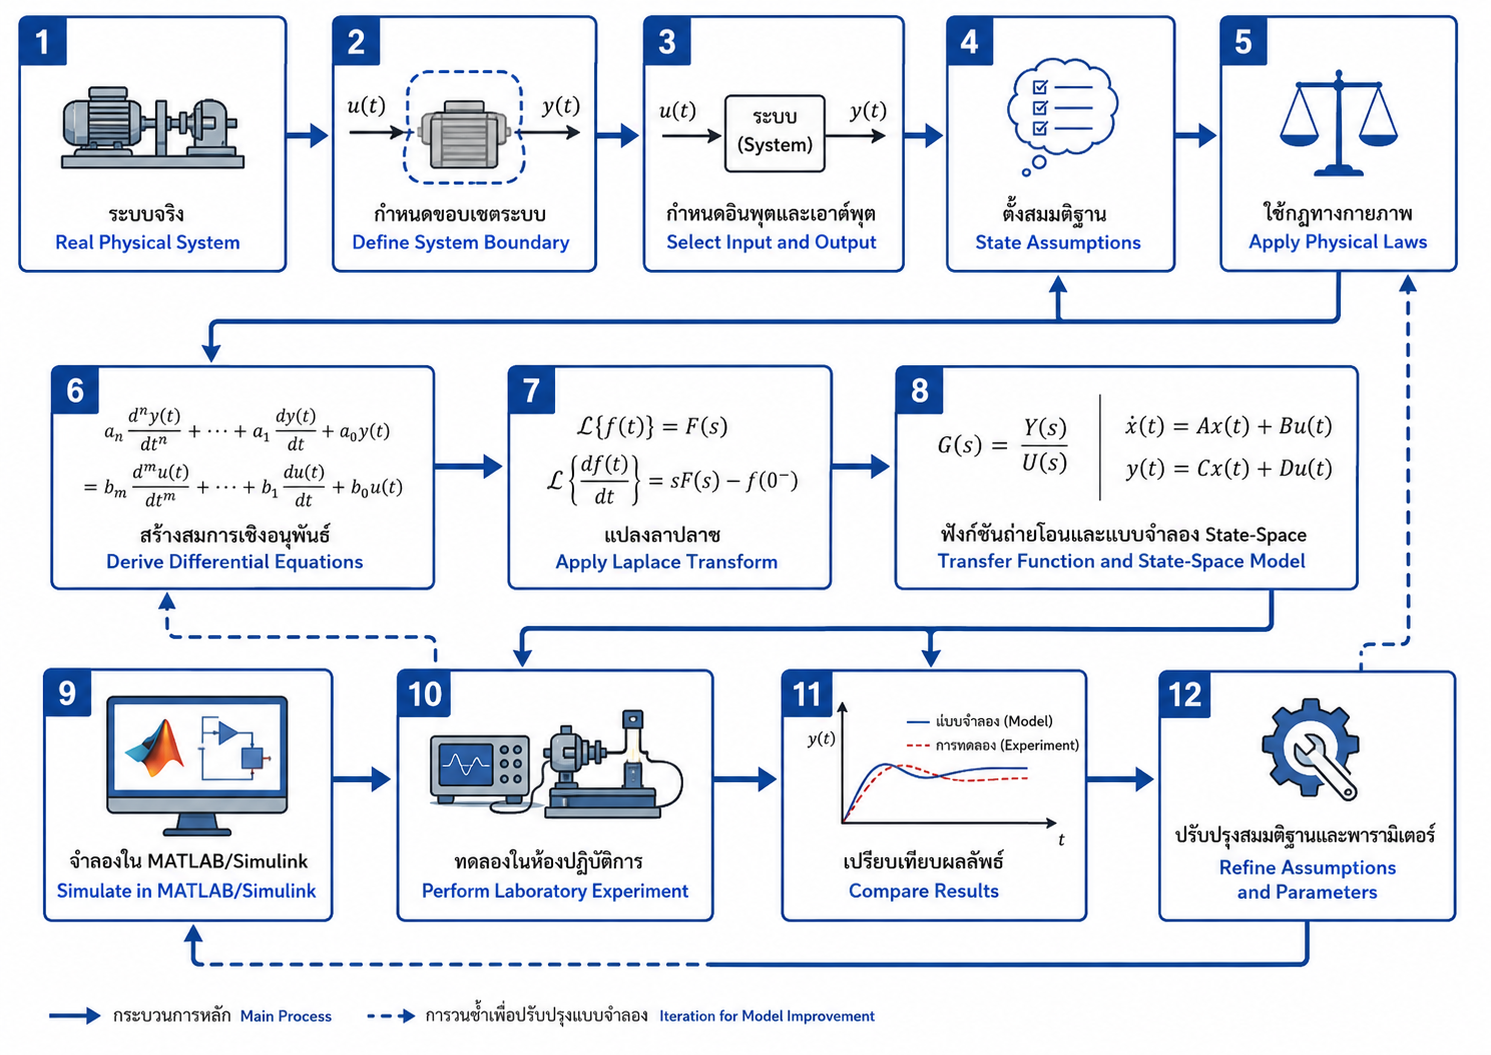
\includegraphics[width=0.8\textwidth]{images/chapter3/figure-1.png}
    \caption{กระบวนการสร้างแบบจำลองระบบควบคุมจากระบบจริงสู่การตรวจสอบแบบจำลอง}
\end{figure}

\par\noindent\rule{\textwidth}{0.4pt}\par

\subsection{6. บทนำ}

การออกแบบระบบควบคุมไม่สามารถเริ่มจากการเลือกตัวควบคุมเพียงอย่างเดียว ผู้วิเคราะห์ต้องทราบก่อนว่าเมื่ออินพุตเปลี่ยน ระบบจริงตอบสนองอย่างไร ตัวอย่างเช่น เมื่อป้อนแรงดันให้มอเตอร์ กระแสจะเพิ่มขึ้นก่อนที่ความเร็วจะเปลี่ยน เมื่อออกแรงต่อระบบมวล–สปริง มวลอาจสั่นและค่อย ๆ หยุดจากผลของแรงหน่วง หรือเมื่อป้อนแรงดันสลับให้วงจร RLC ขนาดและเฟสของแรงดันเอาต์พุตจะเปลี่ยนตามความถี่

การสร้างแบบจำลองจึงเป็นสะพานเชื่อมระหว่างกฎทางฟิสิกส์กับเครื่องมือวิเคราะห์ระบบควบคุม แบบจำลองที่ดีไม่จำเป็นต้องรวมรายละเอียดทุกอย่างของระบบจริง แต่ต้องเก็บลักษณะพลวัตที่สำคัญต่อวัตถุประสงค์ของการศึกษาไว้ ตัวอย่างเช่น หากต้องการศึกษาความเร็วรอบของมอเตอร์ อาจละเลยความยืดหยุ่นของเพลา แต่ต้องคงความเหนี่ยวนำของขดลวด ความต้านทาน โมเมนต์ความเฉื่อย แรงเสียดทาน และแรงเคลื่อนไฟฟ้าย้อนกลับไว้ตามระดับความแม่นยำที่ต้องการ

ความถูกต้องของแบบจำลองจึงขึ้นกับสามองค์ประกอบสำคัญ ได้แก่

\begin{itemize}
    \item การเลือกขอบเขตและตัวแปรที่เหมาะสม
    \item การใช้กฎทางฟิสิกส์และเครื่องหมายอย่างถูกต้อง
    \item การตรวจสอบแบบจำลองกับข้อมูลหรือพฤติกรรมของระบบจริง
\end{itemize}

\par\noindent\rule{\textwidth}{0.4pt}\par

\subsection{7. เนื้อหาหลัก}

\subsubsection{7.1 ความหมายของแบบจำลองทางคณิตศาสตร์ในระบบควบคุม}

\textbf{แบบจำลองทางคณิตศาสตร์} คือ ชุดสมการ ความสัมพันธ์ หรือกฎที่อธิบายพฤติกรรมของระบบด้วยตัวแปรและพารามิเตอร์ แบบจำลองอาจอยู่ในรูปสมการเชิงอนุพันธ์ ฟังก์ชันถ่ายโอน สมการสถานะ แผนภาพบล็อก หรือแบบจำลองเชิงตัวเลข

แบบจำลองในระบบควบคุมมักมุ่งตอบคำถามต่อไปนี้

\begin{enumerate}
    \item อินพุตใดเป็นตัวกระตุ้นระบบ
    \item เอาต์พุตใดเป็นตัวแปรที่ต้องการวัดหรือควบคุม
    \item ระบบสะสมพลังงานหรือข้อมูลไว้ในองค์ประกอบใด
    \item พารามิเตอร์ใดกำหนดความเร็ว การสั่น การหน่วง และอัตราขยายของระบบ
    \item แบบจำลองมีความถูกต้องในช่วงการทำงานใด
\end{enumerate}

\paragraph{7.1.1 แบบจำลองเชิงกายภาพและแบบจำลองเชิงข้อมูล}

\begin{itemize}
    \item \textbf{แบบจำลองเชิงกายภาพ (Physics-Based Model)} สร้างจากกฎทางกล ไฟฟ้า ความร้อน หรือของไหล พารามิเตอร์มักมีความหมายทางกายภาพชัดเจน
    \item \textbf{แบบจำลองเชิงข้อมูล (Data-Driven Model)} สร้างจากข้อมูลอินพุต–เอาต์พุตที่วัดได้ โดยประมาณโครงสร้างและพารามิเตอร์ให้สอดคล้องกับข้อมูล
\end{itemize}

บทนี้เน้นแบบจำลองเชิงกายภาพ เพราะช่วยให้ผู้เรียนเข้าใจว่าพฤติกรรมพลวัตเกิดจากองค์ประกอบใด และสามารถติดตามที่มาของสมการได้

\paragraph{7.1.2 ขั้นตอนทั่วไปในการสร้างแบบจำลอง}

\begin{enumerate}
    \item กำหนดวัตถุประสงค์ของแบบจำลอง
    \item กำหนดขอบเขตของระบบ
    \item เลือกอินพุต เอาต์พุต และตัวแปรภายใน
    \item กำหนดทิศทางบวก จุดอ้างอิง และเครื่องหมาย
    \item ระบุสมมติฐานและเงื่อนไขการทำงาน
    \item ใช้กฎทางฟิสิกส์สร้างสมการ
    \item จัดรูปเป็นสมการเชิงอนุพันธ์
    \item แปลงเป็นฟังก์ชันถ่ายโอนหรือสมการสถานะ
    \item ตรวจสอบหน่วย อันดับ และพฤติกรรมขอบเขต
    \item เปรียบเทียบกับการจำลองหรือผลทดลองและปรับปรุงแบบจำลอง
\end{enumerate}

\paragraph{7.1.3 สมมติฐานที่พบบ่อย}

\begin{itemize}
    \item พารามิเตอร์คงที่ตามเวลา
    \item องค์ประกอบทำงานในช่วงเชิงเส้น
    \item ไม่มีการอิ่มตัว ฮิสเทอรีซิส หรือเดดโซน
    \item ไม่มีความล่าช้าที่ไม่ได้ระบุ
    \item สายไฟและจุดต่อเป็นอุดมคติ
    \item มวล สปริง ตัวหน่วง ตัวต้านทาน ตัวเหนี่ยวนำ และตัวเก็บประจุเป็นองค์ประกอบรวมศูนย์
    \item ผลของสัญญาณรบกวนและความไม่แน่นอนถูกละเลยในแบบจำลองเริ่มต้น
\end{itemize}

แบบจำลองที่มีสมมติฐานมากเกินไปอาจง่ายต่อการวิเคราะห์แต่ไม่สอดคล้องกับระบบจริง ขณะที่แบบจำลองละเอียดเกินไปอาจซับซ้อนโดยไม่เพิ่มประโยชน์ต่อวัตถุประสงค์การควบคุม

\par\noindent\rule{\textwidth}{0.4pt}\par

\subsubsection{7.2 สมการเชิงอนุพันธ์และการแปลงลาปลาซ}

สมการเชิงอนุพันธ์แสดงความสัมพันธ์ระหว่างอินพุต เอาต์พุต และอนุพันธ์ตามเวลา สำหรับระบบเชิงเส้นไม่แปรตามเวลาทั่วไป อาจเขียนได้เป็น

\[
a_n\frac{d^n y(t)}{dt^n}+a_{n-1}\frac{d^{n-1}y(t)}{dt^{n-1}}+\cdots+a_1\frac{dy(t)}{dt}+a_0y(t)
=
b_m\frac{d^m u(t)}{dt^m}+\cdots+b_1\frac{du(t)}{dt}+b_0u(t)
\]

โดยที่

\begin{itemize}
    \item $u(t)$ คืออินพุต
    \item $y(t)$ คือเอาต์พุต
    \item $a_i$ และ $b_i$ คือสัมประสิทธิ์คงที่
    \item $n$ คืออันดับสูงสุดของอนุพันธ์เอาต์พุต
\end{itemize}

เมื่อใช้การแปลงลาปลาซกับอนุพันธ์อันดับหนึ่ง จะได้

\[
\mathcal{L}\left\{\frac{dy(t)}{dt}\right\}=sY(s)-y(0^-)
\]

และสำหรับอนุพันธ์อันดับสอง

\[
\mathcal{L}\left\{\frac{d^2y(t)}{dt^2}\right\}=s^2Y(s)-sy(0^-)-\dot{y}(0^-)
\]

หากกำหนดค่าเริ่มต้นเป็นศูนย์ สมการอนุพันธ์จะเปลี่ยนเป็นสมการพีชคณิตใน $s$ เช่น

\[
a_ns^nY(s)+a_{n-1}s^{n-1}Y(s)+\cdots+a_0Y(s)
=
\left(b_ms^m+\cdots+b_0\right)U(s)
\]

% [รูปที่ 2: การเชื่อมโยงโดเมนเวลาและโดเมน $s$]
% ประเภทภาพ: Infographic / Equation Map
% ตำแหน่งที่แนะนำ: หลังหัวข้อ 7.2
% วัตถุประสงค์การเรียนรู้: แสดงว่าการแปลงลาปลาซเปลี่ยนอนุพันธ์เป็นพหุนามของ $s$ อย่างไร
% คำอธิบายภาพ: ด้านซ้ายเป็นสมการเชิงอนุพันธ์ในเวลา ตรงกลางเป็นลูกศร Laplace Transform พร้อมเงื่อนไข zero initial conditions ด้านขวาเป็นสมการพีชคณิตและอัตราส่วน $G(s)=Y(s)/U(s)$
% องค์ประกอบที่ต้องมี: $y(t)$, $u(t)$, อนุพันธ์, $Y(s)$, $U(s)$, พหุนามของ $s$, เงื่อนไขค่าเริ่มต้นเป็นศูนย์
% ข้อความหรือป้ายกำกับ: Time Domain, Laplace Transform, $s$-Domain, Zero Initial Conditions
% ภาษาของป้ายกำกับ: ไทยและอังกฤษ
% สัดส่วนภาพ: 16:9
% Image Generation Prompt: Educational equation-map infographic connecting a linear differential equation in the time domain to an algebraic equation in the Laplace s-domain. Show input u(t), output y(t), first and second derivatives, a central arrow labeled Laplace Transform with zero initial conditions, and the resulting ratio G(s)=Y(s)/U(s). Clean engineering textbook layout, bilingual Thai-English labels, white background, dark blue equations.
% Alt Text: ภาพแสดงการใช้ลาปลาซเปลี่ยนสมการเชิงอนุพันธ์ในเวลาเป็นฟังก์ชันถ่ายโอนในโดเมนเอส

\begin{figure}[htbp]
    \centering
    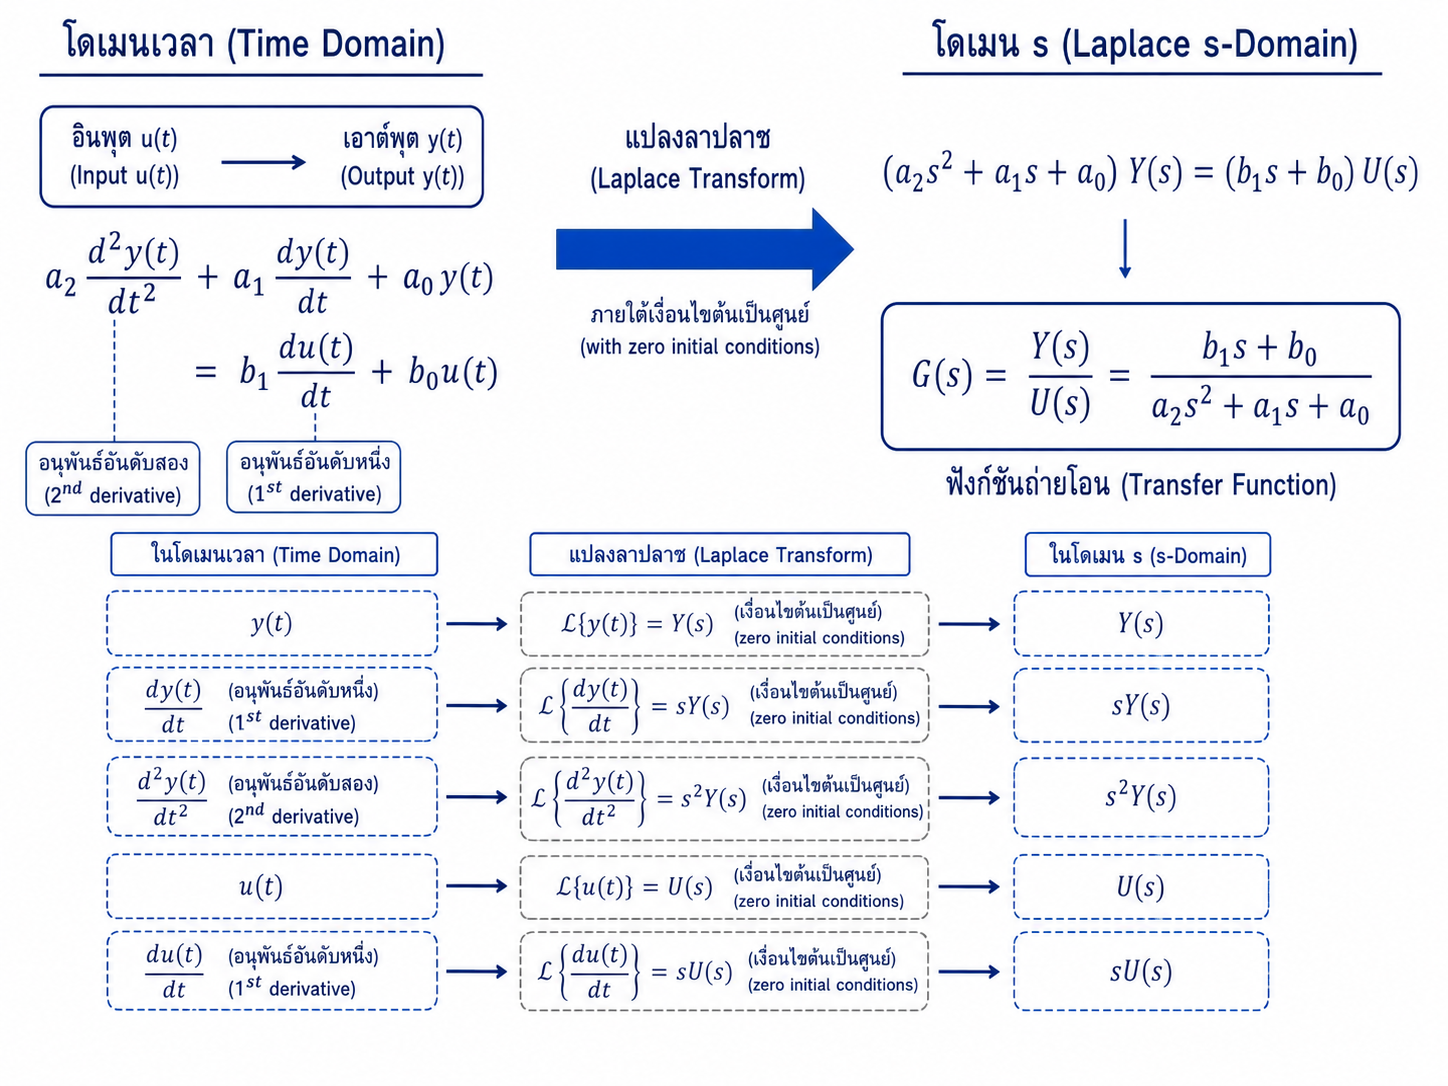
\includegraphics[width=0.8\textwidth]{images/chapter3/figure-2.png}
    \caption{การเชื่อมโยงโดเมนเวลาและโดเมน $s$}
\end{figure}

\par\noindent\rule{\textwidth}{0.4pt}\par

\subsubsection{7.3 นิยามและเงื่อนไขของฟังก์ชันถ่ายโอน}

สำหรับระบบเชิงเส้นไม่แปรตามเวลาที่มีอินพุต $u(t)$ และเอาต์พุต $y(t)$ ฟังก์ชันถ่ายโอนนิยามเป็นอัตราส่วนในโดเมนลาปลาซภายใต้ค่าเริ่มต้นเป็นศูนย์ (MathWorks, n.d.)

\[
G(s)=\frac{Y(s)}{U(s)}\bigg|_{\text{initial conditions}=0}
\]

ฟังก์ชันถ่ายโอนทั่วไปเขียนได้เป็น

\[
G(s)=\frac{b_ms^m+b_{m-1}s^{m-1}+\cdots+b_1s+b_0}
{a_ns^n+a_{n-1}s^{n-1}+\cdots+a_1s+a_0}
\]

\paragraph{7.3.1 ความหมายของตัวแปรและหน่วย}

\begin{itemize}
    \item $s=\sigma+j\omega$ เป็นตัวแปรเชิงซ้อน หน่วยโดยทั่วไปเทียบเท่า $\text{s}^{-1}$
    \item $Y(s)$ และ $U(s)$ เป็นการแปลงลาปลาซของเอาต์พุตและอินพุต
    \item หน่วยของ $G(s)$ ขึ้นกับชนิดของอินพุตและเอาต์พุต เช่น $\text{m/N}$, $\text{rad}\,\text{s}^{-1}\text{/V}$ หรือไม่มีหน่วย
\end{itemize}

\paragraph{7.3.2 เงื่อนไขการใช้ Transfer Function}

\begin{enumerate}
    \item ระบบต้องเป็นเชิงเส้น หรือถูกทำให้เป็นเชิงเส้นรอบจุดทำงาน
    \item พารามิเตอร์ของระบบต้องไม่แปรตามเวลาในช่วงที่พิจารณา
    \item นิยามมาตรฐานใช้ค่าเริ่มต้นเป็นศูนย์
    \item ต้องระบุอินพุตและเอาต์พุตให้ชัดเจน เพราะระบบเดียวกันอาจมีฟังก์ชันถ่ายโอนต่างกันเมื่อเปลี่ยนเอาต์พุต
    \item สำหรับการใช้งานพื้นฐานในบทนี้ เน้นระบบอินพุตเดียวเอาต์พุตเดียว
    \item พหุนามส่วนต้องไม่เป็นศูนย์ทุกสัมประสิทธิ์ และควรจัดเรียงตามกำลังของ $s$
    \item ในแบบจำลองที่นำไปใช้กับบล็อก Transfer Fcn โดยตรง โดยทั่วไปอันดับส่วนต้องไม่น้อยกว่าอันดับเศษ
\end{enumerate}

\paragraph{7.3.3 ความหมายทางกายภาพ}

ฟังก์ชันถ่ายโอนไม่ได้หมายถึงการหารสัญญาณในโดเมนเวลา แต่เป็นตัวดำเนินการเชิงพลวัตที่บอกว่าองค์ประกอบของสัญญาณอินพุตถูกขยาย ลดทอน หน่วงเฟส หรือเปลี่ยนรูปอย่างไร เมื่อใช้ร่วมกับอินพุตในโดเมน $s$ จะได้

\[
Y(s)=G(s)U(s)
\]

\paragraph{7.3.4 โพล ซีโร และอันดับของระบบ}

\begin{itemize}
    \item \textbf{ซีโร (Zeros)} คือค่าของ $s$ ที่ทำให้พหุนามเศษเป็นศูนย์
    \item \textbf{โพล (Poles)} คือค่าของ $s$ ที่ทำให้พหุนามส่วนเป็นศูนย์
    \item \textbf{อันดับของระบบ} โดยทั่วไปสัมพันธ์กับกำลังสูงสุดของพหุนามส่วนหลังตัดตัวประกอบร่วมแล้ว
\end{itemize}

โพลสัมพันธ์อย่างใกล้ชิดกับรูปแบบการตอบสนองตามเวลา ส่วนซีโรมีผลต่อรูปร่าง ขนาด และเฟสของการตอบสนอง อย่างไรก็ตาม การวิเคราะห์เสถียรภาพและการตอบสนองเชิงลึกจะศึกษาในบทถัดไป

\paragraph{7.3.5 ข้อจำกัด}

\begin{itemize}
    \item ไม่แสดงสภาวะภายในทั้งหมดของระบบ
    \item ไม่รวมผลจากค่าเริ่มต้นที่ไม่เป็นศูนย์ไว้ในนิยาม
    \item แบบจำลองเชิงเส้นอาจไม่ถูกต้องเมื่อระบบอิ่มตัวหรือทำงานไกลจากจุดทำงาน
    \item ระบบที่มีพารามิเตอร์เปลี่ยนตามเวลาและระบบไม่เชิงเส้นต้องใช้วิธีอื่นหรือสร้างแบบจำลองประมาณ
    \item การแทนระบบหลายอินพุตหลายเอาต์พุตต้องใช้เมทริกซ์ของฟังก์ชันถ่ายโอนหรือสมการสถานะ
\end{itemize}

\paragraph{7.3.6 ตัวอย่างพื้นฐาน: จากสมการเชิงอนุพันธ์เป็น Transfer Function}

\textbf{ตัวอย่างเพิ่มเติมเพื่อการเรียนรู้}\\กำหนดระบบ

\[
2\ddot{y}(t)+5\dot{y}(t)+3y(t)=4u(t)
\]

\textbf{ขั้นที่ 1 วิเคราะห์ระบบ}\\อินพุตคือ $u(t)$ และเอาต์พุตคือ $y(t)$ ระบบเป็นสมการเชิงเส้นอันดับสอง

\textbf{ขั้นที่ 2 กำหนดเงื่อนไข}\\ใช้ค่าเริ่มต้นเป็นศูนย์ คือ $y(0^-)=0$ และ $\dot{y}(0^-)=0$

\textbf{ขั้นที่ 3 แปลงลาปลาซ}

\[
2s^2Y(s)+5sY(s)+3Y(s)=4U(s)
\]

\textbf{ขั้นที่ 4 จัดรูป}

\[
\left(2s^2+5s+3\right)Y(s)=4U(s)
\]

ดังนั้น

\[
G(s)=\frac{Y(s)}{U(s)}=\frac{4}{2s^2+5s+3}
\]

\textbf{ตรวจสอบ}\\อันดับของระบบเท่ากับ 2 และหน่วยของฟังก์ชันถ่ายโอนขึ้นกับหน่วยของ $y$ และ $u$

\par\noindent\rule{\textwidth}{0.4pt}\par

\subsubsection{7.4 การสร้างแบบจำลองระบบทางกล}

ระบบทางกลเชิงเส้นที่พบบ่อยประกอบด้วยมวล สปริง และตัวหน่วงหนืด

\begin{table}[htbp]
    \centering
    \begin{tabular}{l l l l}
        \hline
        \textbf{องค์ประกอบ} & \textbf{ความสัมพันธ์ในโดเมนเวลา} & \textbf{พารามิเตอร์และหน่วย} & \textbf{ความหมาย} \\
        \hline
        มวล & $F_m(t)=m\ddot{x}(t)$ & $m$ หน่วย kg & ต้านการเปลี่ยนแปลงความเร็ว \\
        สปริง & $F_k(t)=kx(t)$ & $k$ หน่วย N/m & สะสมพลังงานศักย์และสร้างแรงคืนตัว \\
        ตัวหน่วง & $F_c(t)=c\dot{x}(t)$ & $c$ หน่วย N·s/m & สลายพลังงานและลดการสั่น \\
        \hline
    \end{tabular}
\end{table}

\paragraph{7.4.1 การกำหนดทิศทางและ Free-Body Diagram}

ก่อนเขียนสมการ ต้องกำหนดทิศทางบวกของการกระจัด $x(t)$ และวาดแรงทั้งหมดบนมวล หากกำหนดทิศทางบวกไปทางขวา แรงสปริงและแรงหน่วงที่ต้านการเคลื่อนที่จะมีเครื่องหมายตรงข้ามกับ $x(t)$ และ $\dot{x}(t)$ ตามลำดับ

% [รูปที่ 3: ระบบมวล–สปริง–ตัวหน่วงและแผนภาพแรง]
% ประเภทภาพ: Technical Illustration
% ตำแหน่งที่แนะนำ: ก่อนสมการระบบมวล–สปริง–ตัวหน่วง
% วัตถุประสงค์การเรียนรู้: ช่วยกำหนดแรง ทิศทาง และเครื่องหมายก่อนสร้างสมการ
% คำอธิบายภาพ: แสดงมวล $m$ บนพื้นราบ เชื่อมกับผนังด้วยสปริง $k$ และตัวหน่วง $c$ แบบขนาน มีแรงอินพุต $F(t)$ ไปทางขวา การกระจัด $x(t)$ ไปทางขวา และภาพย่อย Free-Body Diagram ของมวลพร้อมแรง $F(t)$, $kx(t)$ และ $c\dot{x}(t)$
% องค์ประกอบที่ต้องมี: ผนัง มวล สปริง ตัวหน่วง ลูกศรแรง ลูกศรการกระจัด และแกนอ้างอิง
% ข้อความหรือป้ายกำกับ: $m$, $k$, $c$, $F(t)$, $x(t)$, $kx(t)$, $c\dot{x}(t)$
% ภาษาของป้ายกำกับ: สัญลักษณ์สากลและอังกฤษ
% สัดส่วนภาพ: 16:9
% Image Generation Prompt: Mechanical engineering textbook diagram of a translational mass-spring-damper system. A mass m rests on a horizontal frictionless surface and is connected to a fixed wall by a spring k and viscous damper c in parallel. An external force F(t) acts to the right and displacement x(t) is positive to the right. Include a separate free-body diagram of the mass showing F(t) to the right and restoring forces kx(t) and c x-dot(t) to the left. Clean black line art, white background, accurate technical symbols.
% Alt Text: ระบบมวลต่อกับสปริงและตัวหน่วง พร้อมแผนภาพแรงที่ใช้สร้างสมการการเคลื่อนที่

\begin{figure}[htbp]
    \centering
    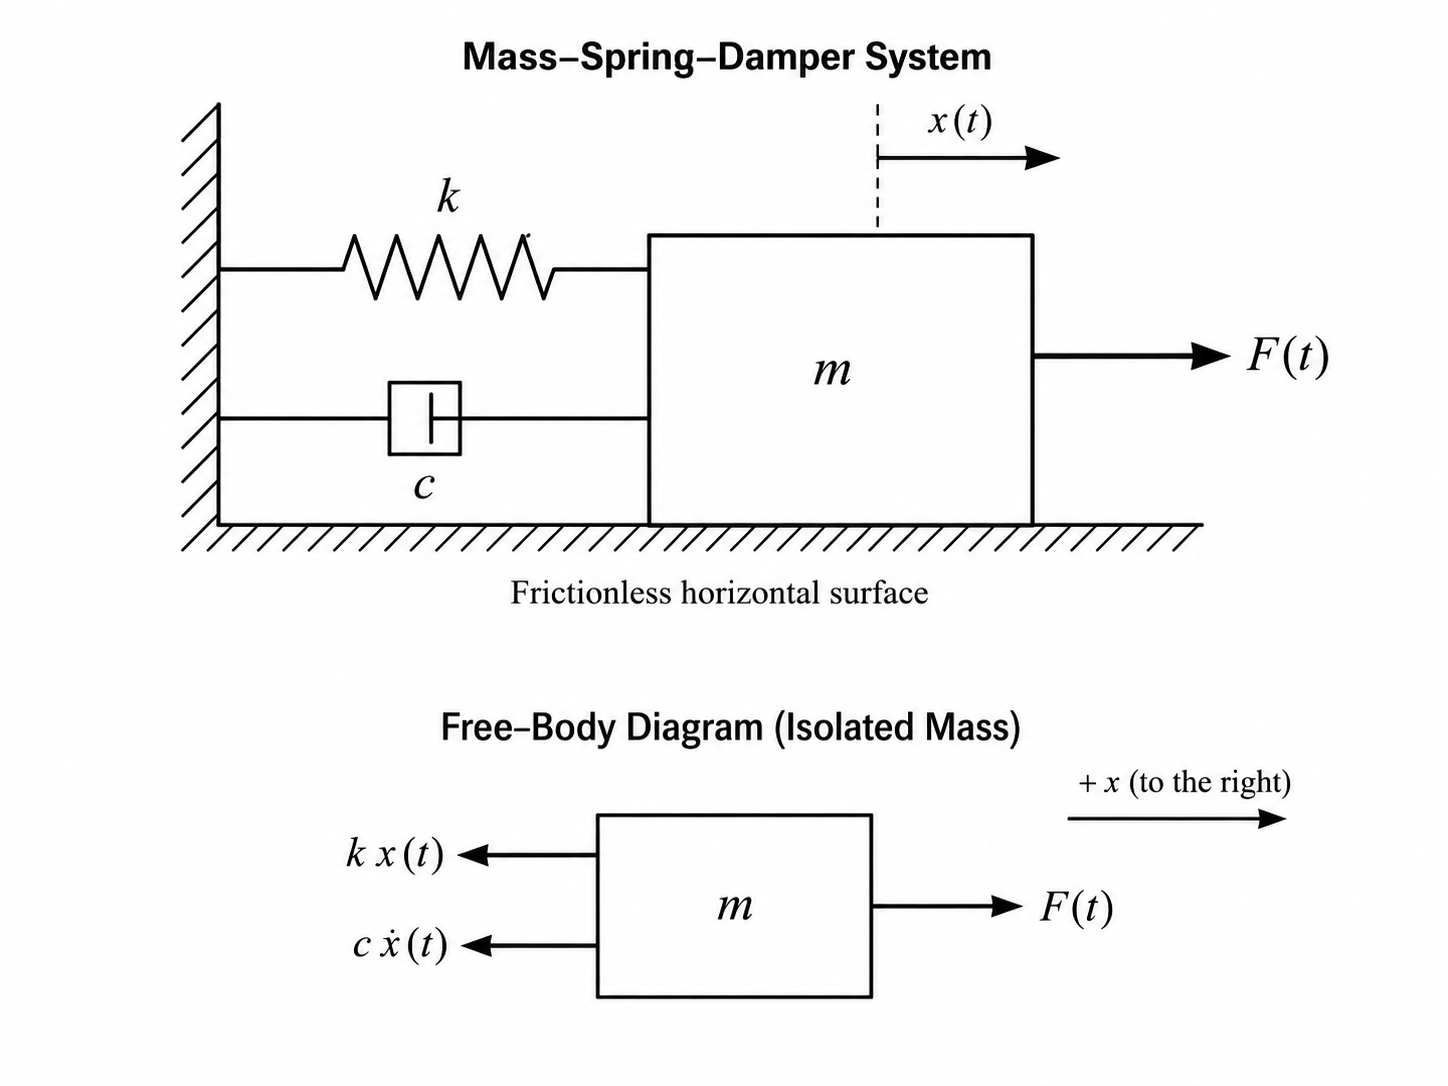
\includegraphics[width=0.8\textwidth]{images/chapter3/figure-3.png}
    \caption{ระบบมวล–สปริง–ตัวหน่วงและแผนภาพแรง}
\end{figure}

\paragraph{7.4.2 สมการของระบบมวล–สปริง–ตัวหน่วง}

ใช้กฎข้อที่สองของนิวตัน

\[
\sum F(t)=m\ddot{x}(t)
\]

เมื่อรวมแรงในทิศบวก จะได้

\[
F(t)-c\dot{x}(t)-kx(t)=m\ddot{x}(t)
\]

จัดรูปเป็น

\[
m\ddot{x}(t)+c\dot{x}(t)+kx(t)=F(t)
\]

ภายใต้ค่าเริ่มต้นเป็นศูนย์

\[
\left(ms^2+cs+k\right)X(s)=F(s)
\]

ดังนั้น ฟังก์ชันถ่ายโอนจากแรงไปยังการกระจัดคือ

\[
G_x(s)=\frac{X(s)}{F(s)}=\frac{1}{ms^2+cs+k}
\]

หากเลือกความเร็ว $v(t)=\dot{x}(t)$ เป็นเอาต์พุต จะได้

\[
G_v(s)=\frac{V(s)}{F(s)}=\frac{s}{ms^2+cs+k}
\]

สมการทั้งสองอธิบายระบบทางกายภาพเดียวกัน แต่แตกต่างกันเพราะเลือกเอาต์พุตต่างกัน

\paragraph{7.4.3 พารามิเตอร์มาตรฐานของระบบอันดับสอง}

หารสมการส่วนด้วย $m$

\[
G_x(s)=\frac{1/m}{s^2+\frac{c}{m}s+\frac{k}{m}}
\]

เปรียบเทียบกับรูปมาตรฐาน

\[
s^2+2\zeta\omega_n s+\omega_n^2
\]

จะได้

\[
\omega_n=\sqrt{\frac{k}{m}}
\]

และ

\[
\zeta=\frac{c}{2\sqrt{mk}}
\]

โดย $\omega_n$ คือความถี่ธรรมชาติไม่หน่วง หน่วย rad/s และ $\zeta$ คืออัตราส่วนการหน่วงซึ่งไม่มีหน่วย

\paragraph{7.4.4 ตัวอย่างบังคับ: ระบบมวล–สปริง–ตัวหน่วง}

\textbf{ตัวอย่างเพิ่มเติมเพื่อการเรียนรู้}\\กำหนด $m=2\ \text{kg}$, $c=6\ \text{N·s/m}$, $k=8\ \text{N/m}$ อินพุตเป็นแรง $F(t)$ และเอาต์พุตเป็นการกระจัด $x(t)$

\textbf{1. วิเคราะห์ระบบ}\\ระบบมีองค์ประกอบสะสมพลังงานสองชนิด คือมวลและสปริง จึงคาดว่าเป็นระบบอันดับสอง

\textbf{2. กำหนดทิศทาง}\\กำหนด $x(t)$ และ $F(t)$ เป็นบวกไปทางขวา

\textbf{3. ใช้กฎของนิวตัน}

\[
2\ddot{x}(t)+6\dot{x}(t)+8x(t)=F(t)
\]

\textbf{4. แปลงลาปลาซภายใต้ค่าเริ่มต้นเป็นศูนย์}

\[
\left(2s^2+6s+8\right)X(s)=F(s)
\]

\textbf{5. ฟังก์ชันถ่ายโอน}

\[
\boxed{\frac{X(s)}{F(s)}=\frac{1}{2s^2+6s+8}}
\]

\textbf{6. ความถี่ธรรมชาติและอัตราส่วนการหน่วง}

\[
\omega_n=\sqrt{\frac{8}{2}}=2\ \text{rad/s}
\]

\[
\zeta=\frac{6}{2\sqrt{(2)(8)}}=0.75
\]

\textbf{7. ตรวจสอบหน่วยและความสมเหตุสมผล}\\เมื่อ $s=0$ อัตราขยายสภาวะคงตัวคือ $1/k=1/8\ \text{m/N}$ ดังนั้นหากป้อนแรงคงที่ $10\ \text{N}$ การกระจัดสภาวะคงตัวตามแบบจำลองคือ

\[
x_{ss}=\frac{10}{8}=1.25\ \text{m}
\]

ค่าดังกล่าวมีขนาดค่อนข้างมาก จึงชี้ให้เห็นว่าสปริงตัวอย่างมีค่าความแข็งต่ำ หากเป็นระบบจริงอาจต้องตรวจสอบว่าการยืดอยู่ในช่วงเชิงเส้นของสปริงหรือไม่

\paragraph{7.4.5 ระบบเชิงหมุนโดยสังเขป}

ระบบเชิงหมุนใช้ความสัมพันธ์ที่คล้ายกัน

\begin{table}[htbp]
    \centering
    \begin{tabular}{l l}
        \hline
        \textbf{การเลื่อนที่} & \textbf{การหมุน} \\
        \hline
        แรง $F$ & แรงบิด $T$ \\
        มวล $m$ & โมเมนต์ความเฉื่อย $J$ \\
        การกระจัด $x$ & มุม $\theta$ \\
        ความเร็ว $\dot{x}$ & ความเร็วเชิงมุม $\omega=\dot{\theta}$ \\
        สัมประสิทธิ์หน่วง $c$ & สัมประสิทธิ์เสียดทานหนืด $b$ \\
        \hline
    \end{tabular}
\end{table}

สมการพื้นฐานคือ

\[
J\ddot{\theta}(t)+b\dot{\theta}(t)+k_\theta\theta(t)=T(t)
\]

\subsubsection{7.5 การสร้างแบบจำลองระบบทางไฟฟ้า}

การสร้างแบบจำลองระบบทางไฟฟ้าเริ่มจากการเลือกแรงดันหรือกระแสที่เป็นอินพุตและเอาต์พุต กำหนดขั้วแรงดันและทิศทางกระแส แล้วใช้กฎแรงดันของเคอร์ชอฟฟ์ (Kirchhoff’s Voltage Law: KVL) หรือกฎกระแสของเคอร์ชอฟฟ์ (Kirchhoff’s Current Law: KCL) ร่วมกับความสัมพันธ์ของอุปกรณ์

\begin{table}[htbp]
    \centering
    \begin{tabular}{l l l l}
        \hline
        \textbf{อุปกรณ์} & \textbf{ความสัมพันธ์ในโดเมนเวลา} & \textbf{อิมพีแดนซ์ในโดเมน $s$ ภายใต้ค่าเริ่มต้นเป็นศูนย์} & \textbf{หน่วยพารามิเตอร์} \\
        \hline
        ตัวต้านทาน $R$ & $v_R(t)=Ri_R(t)$ & $Z_R(s)=R$ & $\Omega$ \\
        ตัวเหนี่ยวนำ $L$ & $v_L(t)=L\dfrac{di_L(t)}{dt}$ & $Z_L(s)=sL$ & H \\
        ตัวเก็บประจุ $C$ & $i_C(t)=C\dfrac{dv_C(t)}{dt}$ & $Z_C(s)=\dfrac{1}{sC}$ & F \\
        \hline
    \end{tabular}
\end{table}

\begin{quote}
\textbf{ข้อควรระวัง:} การใช้ $Z_L=sL$ และ $Z_C=1/(sC)$ ในรูปอย่างง่ายนี้ตั้งอยู่บนสมมติฐานค่าเริ่มต้นเป็นศูนย์ หากตัวเหนี่ยวนำมีกระแสเริ่มต้นหรือตัวเก็บประจุมีแรงดันเริ่มต้น ต้องเพิ่มพจน์ที่เกิดจากพลังงานเริ่มต้นในสมการลาปลาซ
\end{quote}

\paragraph{7.5.1 วงจร RC อนุกรม: เอาต์พุตคร่อมตัวเก็บประจุ}

พิจารณาวงจรที่มีตัวต้านทาน $R$ ต่ออนุกรมกับตัวเก็บประจุ $C$ อินพุตคือ $v_i(t)$ และเอาต์พุตคือแรงดันคร่อมตัวเก็บประจุ $v_o(t)=v_C(t)$

จาก KVL

\[
v_i(t)=v_R(t)+v_C(t)
\]

กระแสในวงจรเท่ากันทุกองค์ประกอบ และ

\[
i(t)=C\frac{dv_o(t)}{dt}
\]

จึงได้

\[
RC\frac{dv_o(t)}{dt}+v_o(t)=v_i(t)
\]

แปลงลาปลาซภายใต้ค่าเริ่มต้นเป็นศูนย์

\[
(RCs+1)V_o(s)=V_i(s)
\]

ดังนั้น

\[
\boxed{G_{RC}(s)=\frac{V_o(s)}{V_i(s)}=\frac{1}{RCs+1}}
\]

นี่คือระบบอันดับหนึ่งที่มีค่าคงตัวเวลา

\[
\tau=RC
\]

และความถี่ตัดเชิงมุม

\[
\omega_c=\frac{1}{RC}
\]

ที่ความถี่ $\omega_c$ ขนาดอัตราขยายของวงจรอุดมคติเท่ากับ $1/\sqrt{2}$ ของค่าที่ความถี่ต่ำ หรือประมาณ $-3\ \text{dB}$

% [รูปที่ 4: การสร้างแบบจำลองวงจร RC และ RL]
% ประเภทภาพ: Technical Illustration / Circuit Diagram
% ตำแหน่งที่แนะนำ: หัวข้อ 7.5.1–7.5.2
% วัตถุประสงค์การเรียนรู้: ช่วยให้ผู้เรียนระบุอินพุต เอาต์พุต ทิศทางกระแส และตำแหน่งวัดแรงดันก่อนสร้างสมการ
% คำอธิบายภาพ: แบ่งภาพเป็นสองส่วน ด้านซ้ายเป็นวงจร RC อนุกรม โดยวัดเอาต์พุตคร่อมตัวเก็บประจุ ด้านขวาเป็นวงจร RL อนุกรม โดยวัดเอาต์พุตคร่อมตัวต้านทาน แสดงลูกศรกระแสและขั้วแรงดันอย่างชัดเจน
% องค์ประกอบที่ต้องมี: แหล่งสัญญาณ $v_i(t)$, ตัวต้านทาน $R$, ตัวเก็บประจุ $C$, ตัวเหนี่ยวนำ $L$, จุดกราวด์, ลูกศรกระแส $i(t)$, เอาต์พุต $v_o(t)$
% ข้อความหรือป้ายกำกับ: “RC Low-Pass”, “RL Low-Pass”, “Input”, “Output”, $R$, $L$, $C$, $i(t)$
% ภาษาของป้ายกำกับ: อังกฤษ
% สัดส่วนภาพ: 16:9
% Image Generation Prompt: Clean educational electrical engineering diagram with two side-by-side circuits. Left: series RC low-pass circuit driven by voltage source vi(t), resistor R followed by capacitor C to ground, output vo(t) measured across C, current arrow i(t). Right: series RL low-pass circuit driven by vi(t), inductor L followed by resistor R to ground, output vo(t) measured across R, current arrow i(t). Use standard IEC/ANSI circuit symbols, clear polarity marks, white background, textbook line-art style, no decorative elements.
% Alt Text: วงจร RC และ RL อนุกรมที่แสดงตำแหน่งอินพุต เอาต์พุต และทิศทางกระแสสำหรับใช้สร้างสมการ

\begin{figure}[htbp]
    \centering
    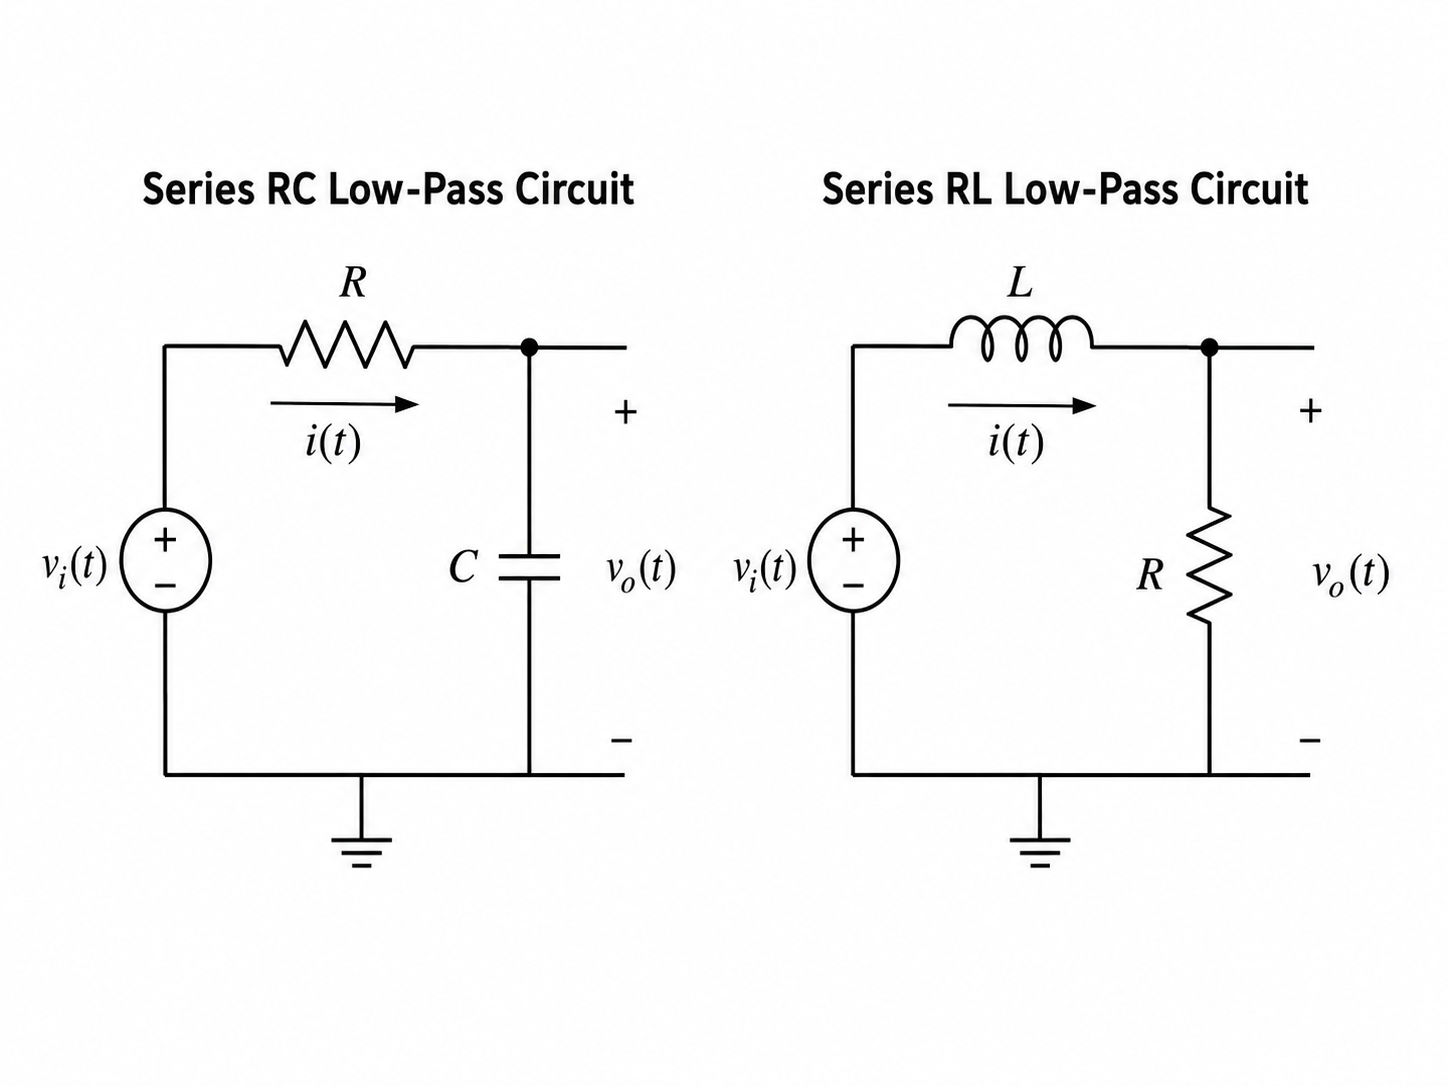
\includegraphics[width=0.8\textwidth]{images/chapter3/figure-4.png}
    \caption{การสร้างแบบจำลองวงจร RC และ RL}
\end{figure}

\paragraph{7.5.2 วงจร RL อนุกรม: เอาต์พุตคร่อมตัวต้านทาน}

จาก KVL

\[
v_i(t)=L\frac{di(t)}{dt}+Ri(t)
\]

เมื่อ $v_o(t)=Ri(t)$ จะได้ $i(t)=v_o(t)/R$ ดังนั้น

\[
\frac{L}{R}\frac{dv_o(t)}{dt}+v_o(t)=v_i(t)
\]

ฟังก์ชันถ่ายโอนคือ

\[
\boxed{G_{RL,R}(s)=\frac{V_o(s)}{V_i(s)}=\frac{R}{Ls+R}
=\frac{1}{\left(\frac{L}{R}\right)s+1}}
\]

ค่าคงตัวเวลาคือ

\[
\tau=\frac{L}{R}
\]

หากเลือกเอาต์พุตคร่อมตัวเหนี่ยวนำแทน จะได้

\[
\boxed{G_{RL,L}(s)=\frac{Ls}{Ls+R}}
\]

ตัวอย่างนี้ย้ำว่า \textbf{วงจรเดียวกันอาจมีฟังก์ชันถ่ายโอนต่างกันตามตำแหน่งเอาต์พุต} วงจรที่วัดคร่อม $R$ มีลักษณะผ่านต่ำ ส่วนวงจรที่วัดคร่อม $L$ มีลักษณะผ่านสูง

\paragraph{7.5.3 วงจร RLC อนุกรม: เอาต์พุตคร่อมตัวเก็บประจุ}

พิจารณาวงจร RLC อนุกรม อินพุตคือ $v_i(t)$ และเอาต์พุตคือ $v_o(t)=v_C(t)$

จาก KVL

\[
v_i(t)=v_R(t)+v_L(t)+v_C(t)
\]

เนื่องจาก

\[
i(t)=C\frac{dv_o(t)}{dt}
\]

จึงมี

\[
v_R(t)=RC\frac{dv_o(t)}{dt}
\]

และ

\[
v_L(t)=LC\frac{d^2v_o(t)}{dt^2}
\]

ดังนั้น

\[
LC\frac{d^2v_o(t)}{dt^2}
+RC\frac{dv_o(t)}{dt}
+v_o(t)=v_i(t)
\]

เมื่อค่าเริ่มต้นเป็นศูนย์

\[
\left(LCs^2+RCs+1\right)V_o(s)=V_i(s)
\]

จึงได้

\[
\boxed{G_{RLC}(s)=\frac{V_o(s)}{V_i(s)}
=\frac{1}{LCs^2+RCs+1}}
\]

หารส่วนด้วย $LC$

\[
G_{RLC}(s)=\frac{1/(LC)}
{s^2+\frac{R}{L}s+\frac{1}{LC}}
\]

เปรียบเทียบกับรูปมาตรฐานอันดับสอง จะได้

\[
\omega_n=\frac{1}{\sqrt{LC}}
\]

\[
\zeta=\frac{R}{2}\sqrt{\frac{C}{L}}
\]

ในวงจรจริงควรแทน $R$ ด้วยความต้านทานอนุกรมรวม

\[
R_{\text{eq}}=R+R_s+r_L+r_{\text{wire}}
\]

เมื่อ $R_s$ คือความต้านทานเอาต์พุตของเครื่องกำเนิดสัญญาณ และ $r_L$ คือความต้านทานขดลวดของตัวเหนี่ยวนำ แบบจำลองที่ละเลยค่าดังกล่าวมักทำนายยอดเรโซแนนซ์สูงกว่าผลทดลอง

% [รูปที่ 5: วงจร RLC อุดมคติและแบบจำลองเชิงปฏิบัติ]
% ประเภทภาพ: Circuit Diagram / Comparative Technical Illustration
% ตำแหน่งที่แนะนำ: หัวข้อ 7.5.3
% วัตถุประสงค์การเรียนรู้: แสดงความแตกต่างระหว่างแบบจำลองอุดมคติกับแบบจำลองที่รวมพารามิเตอร์แฝง
% คำอธิบายภาพ: แสดงวงจร RLC อนุกรมสองวงจรแบบเคียงข้างกัน วงจรแรกใช้ $R$, $L$, $C$ อุดมคติ วงจรที่สองเพิ่ม $R_s$ ของแหล่งกำเนิดและ $r_L$ อนุกรมกับตัวเหนี่ยวนำ พร้อมวัดเอาต์พุตคร่อมตัวเก็บประจุ
% องค์ประกอบที่ต้องมี: แหล่งสัญญาณ, $R_s$, $R$, $r_L$, $L$, $C$, จุดกราวด์, $v_i$, $v_o$, ลูกศรกระแส
% ข้อความหรือป้ายกำกับ: “Ideal Model”, “Practical Model”, “Source Resistance”, “Inductor Winding Resistance”
% ภาษาของป้ายกำกับ: อังกฤษ
% สัดส่วนภาพ: 16:9
% Image Generation Prompt: Engineering textbook comparison of two series RLC low-pass circuits. Left panel labeled Ideal Model: source vi, resistor R, ideal inductor L, capacitor C to ground, output vo across C. Right panel labeled Practical Model: include source resistance Rs and inductor winding resistance rL in series in addition to R, L, C; output vo across C. Show current direction and voltage polarity. Use accurate circuit symbols, clean monochrome line art, white background.
% Alt Text: เปรียบเทียบวงจร RLC อุดมคติกับวงจรที่รวมความต้านทานแหล่งกำเนิดและความต้านทานขดลวด

\begin{figure}[htbp]
    \centering
    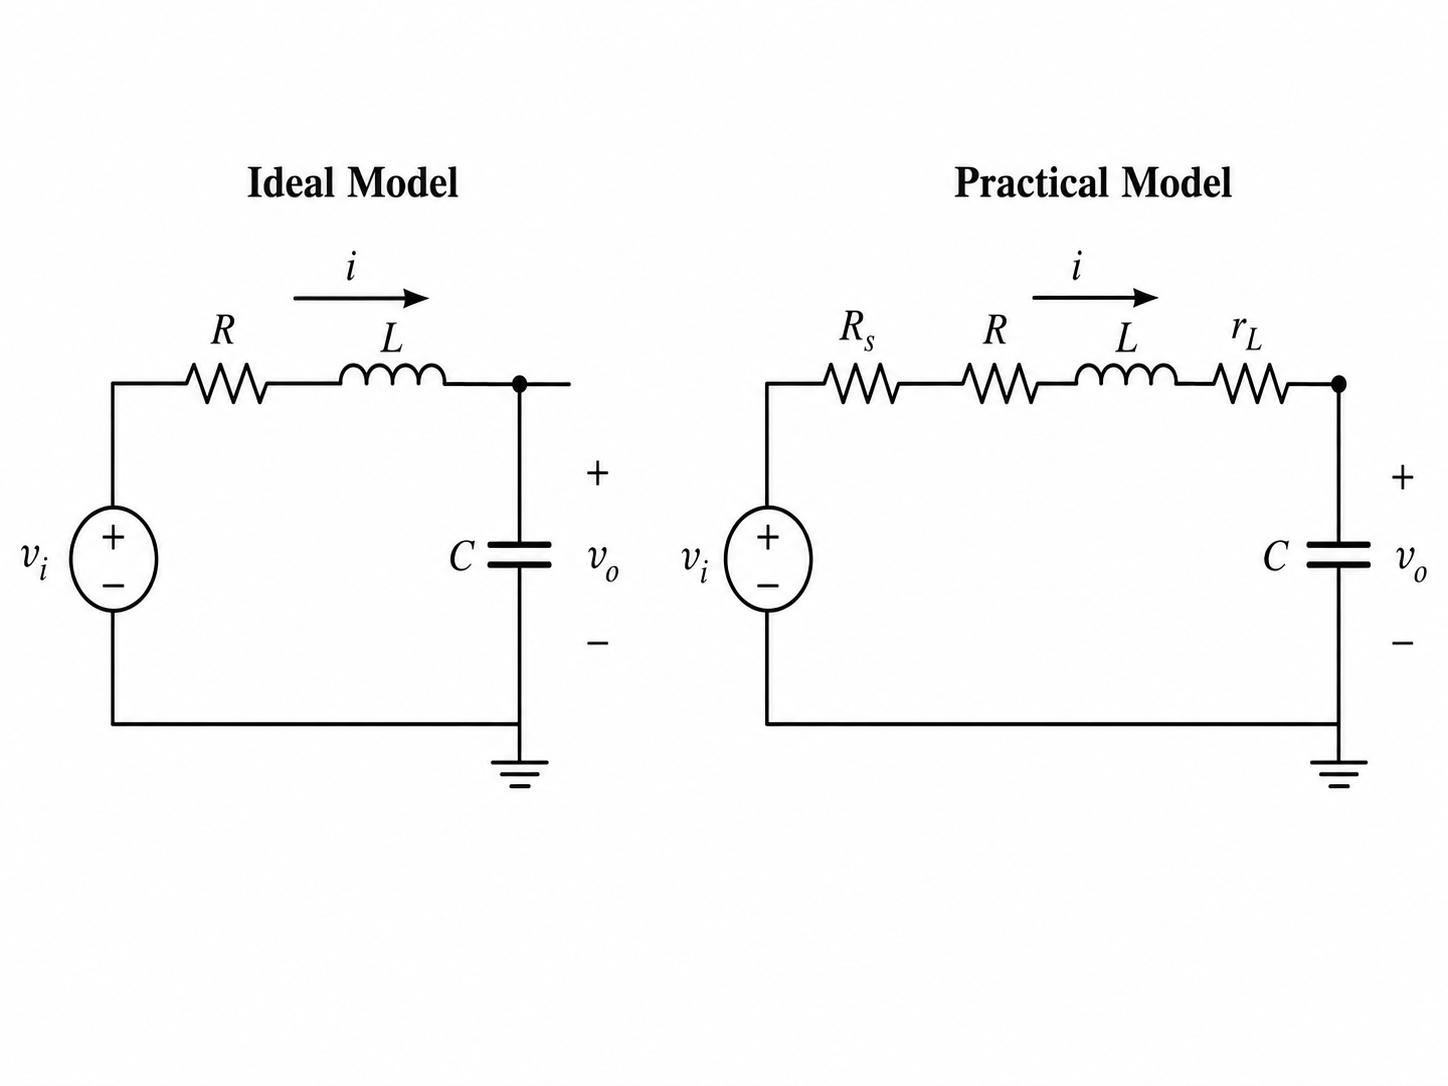
\includegraphics[width=0.8\textwidth]{images/chapter3/figure-5.png}
    \caption{วงจร RLC อุดมคติและแบบจำลองเชิงปฏิบัติ}
\end{figure}

\paragraph{7.5.4 ตัวอย่างบังคับ: หาฟังก์ชันถ่ายโอนของวงจร RLC}

\textbf{ตัวอย่างเพิ่มเติมเพื่อการเรียนรู้}\\กำหนด $R=100\ \Omega$, $L=10\ \text{mH}$ และ $C=1\ \mu\text{F}$ ต่ออนุกรม วัดเอาต์พุตคร่อมตัวเก็บประจุ

\textbf{1. วิเคราะห์ระบบ}\\ตัวเหนี่ยวนำและตัวเก็บประจุเป็นองค์ประกอบสะสมพลังงานสองตัว ระบบจึงเป็นอันดับสอง

\textbf{2. สร้างสมการ}

\[
LC\frac{d^2v_o}{dt^2}+RC\frac{dv_o}{dt}+v_o=v_i
\]

\textbf{3. แทนค่าพารามิเตอร์}

\[
LC=(10\times10^{-3})(1\times10^{-6})=1\times10^{-8}
\]

\[
RC=(100)(1\times10^{-6})=1\times10^{-4}
\]

จึงได้

\[
10^{-8}\frac{d^2v_o}{dt^2}
+10^{-4}\frac{dv_o}{dt}+v_o=v_i
\]

\textbf{4. แปลงเป็นฟังก์ชันถ่ายโอน}

\[
\boxed{
G(s)=\frac{V_o(s)}{V_i(s)}
=\frac{1}{10^{-8}s^2+10^{-4}s+1}
}
\]

หรือคูณทั้งเศษและส่วนด้วย $10^8$

\[
\boxed{
G(s)=\frac{10^8}{s^2+10^4s+10^8}
}
\]

\textbf{5. คำนวณพารามิเตอร์อันดับสอง}

\[
\omega_n=\frac{1}{\sqrt{LC}}
=\frac{1}{\sqrt{10^{-8}}}
=10{,}000\ \text{rad/s}
\]

\[
f_n=\frac{\omega_n}{2\pi}
\approx1{,}591.55\ \text{Hz}
\]

\[
\zeta=\frac{R}{2}\sqrt{\frac{C}{L}}
=\frac{100}{2}\sqrt{\frac{10^{-6}}{10^{-2}}}
=0.5
\]

ระบบอุดมคติมีการหน่วงต่ำกว่า 1 จึงอาจเกิดยอดเรโซแนนซ์ เมื่อ $\zeta<1/\sqrt{2}$ ความถี่ที่เกิดยอดขนาดโดยประมาณคือ

\[
\omega_r=\omega_n\sqrt{1-2\zeta^2}
=10{,}000\sqrt{0.5}
\approx7{,}071.1\ \text{rad/s}
\]

\[
f_r\approx1{,}125.4\ \text{Hz}
\]

\textbf{6. ตรวจสอบความสมเหตุสมผล}\\ที่ความถี่ศูนย์ ตัวเก็บประจุทำหน้าที่เสมือนวงจรเปิดและแรงดันเอาต์พุตเท่ากับอินพุต จึงมี $G(0)=1$ ซึ่งสอดคล้องกับสมการ

\paragraph{7.5.5 วงจร Op-Amp}

การสร้างแบบจำลองวงจร Op-Amp มักเริ่มจากสมมติฐาน Op-Amp อุดมคติ

\begin{enumerate}
    \item อัตราขยายวงเปิดมีค่ามากมาก
    \item กระแสไหลเข้าสู่ขาอินพุตเป็นศูนย์
    \item เมื่อมีป้อนกลับลบและยังไม่อิ่มตัว จะมี $v_+\approx v_-$
    \item แบนด์วิดท์และอัตราการเปลี่ยนแปลงแรงดันไม่จำกัดในแบบจำลองอุดมคติ
\end{enumerate}

สมมติฐานเหล่านี้ใช้ได้เมื่อวงจรทำงานในช่วงเชิงเส้นและความถี่ไม่สูงเกินข้อจำกัดของอุปกรณ์จริง

\subparagraph{ก. วงจรขยายกลับเฟส}

วงจรขยายกลับเฟสที่ใช้ตัวต้านทานอินพุต $R_{in}$ และตัวต้านทานป้อนกลับ $R_f$ มี

\[
\boxed{
\frac{V_o(s)}{V_i(s)}=-\frac{R_f}{R_{in}}
}
\]

เครื่องหมายลบแสดงการกลับเฟส $180^\circ$

\subparagraph{ข. วงจรขยายกลับเฟสแบบผ่านต่ำอันดับหนึ่ง}

หากต่อ $R_f$ ขนานกับ $C_f$ อิมพีแดนซ์ป้อนกลับคือ

\[
Z_f(s)=R_f\parallel\frac{1}{sC_f}
=\frac{R_f}{1+sR_fC_f}
\]

ดังนั้น

\[
\boxed{
G(s)=-\frac{R_f/R_{in}}{1+sR_fC_f}
}
\]

วงจรนี้มีอัตราขยายความถี่ต่ำ $-R_f/R_{in}$ และมีโพลที่

\[
\omega_p=\frac{1}{R_fC_f}
\]

\subparagraph{ค. วงจรอินทิเกรตอุดมคติ}

เมื่อใช้อิมพีแดนซ์ป้อนกลับเป็นตัวเก็บประจุอย่างเดียว

\[
\boxed{
G(s)=-\frac{1}{R_{in}Cs}
}
\]

วงจรจริงมักเพิ่มตัวต้านทานขนานกับตัวเก็บประจุเพื่อจำกัดอัตราขยายที่ความถี่ต่ำและลดปัญหาการอิ่มตัวจากแรงดันออฟเซต

% [รูปที่ 6: วงจร Op-Amp และฟังก์ชันถ่ายโอน]
% ประเภทภาพ: Circuit Diagram / Infographic
% ตำแหน่งที่แนะนำ: หัวข้อ 7.5.5
% วัตถุประสงค์การเรียนรู้: เชื่อมโยงอิมพีแดนซ์ป้อนกลับกับรูปของฟังก์ชันถ่ายโอน
% คำอธิบายภาพ: แสดงวงจรสามแบบ ได้แก่ inverting amplifier, first-order active low-pass และ practical integrator พร้อมสมการฟังก์ชันถ่ายโอนใต้แต่ละวงจร
% องค์ประกอบที่ต้องมี: สัญลักษณ์ Op-Amp, $R_{in}$, $R_f$, $C_f$, กราวด์, $v_i$, $v_o$, ขา $+$ และ $-$
% ข้อความหรือป้ายกำกับ: ชื่อวงจรทั้งสามและสมการกำกับแบบสั้น
% ภาษาของป้ายกำกับ: อังกฤษ
% สัดส่วนภาพ: 16:9
% Image Generation Prompt: Clean educational comparison of three ideal op-amp circuits: inverting amplifier with Rin and Rf; first-order inverting active low-pass with Rf parallel Cf; practical integrator with capacitor Cf parallel a large resistor Rf. Label vi, vo, plus and minus inputs, component values, and place the corresponding transfer function below each circuit. Accurate circuit symbols, white background, engineering textbook style.
% Alt Text: วงจร Op-Amp สามแบบที่แสดงความสัมพันธ์ระหว่างอุปกรณ์ป้อนกลับและฟังก์ชันถ่ายโอน

\begin{figure}[htbp]
    \centering
    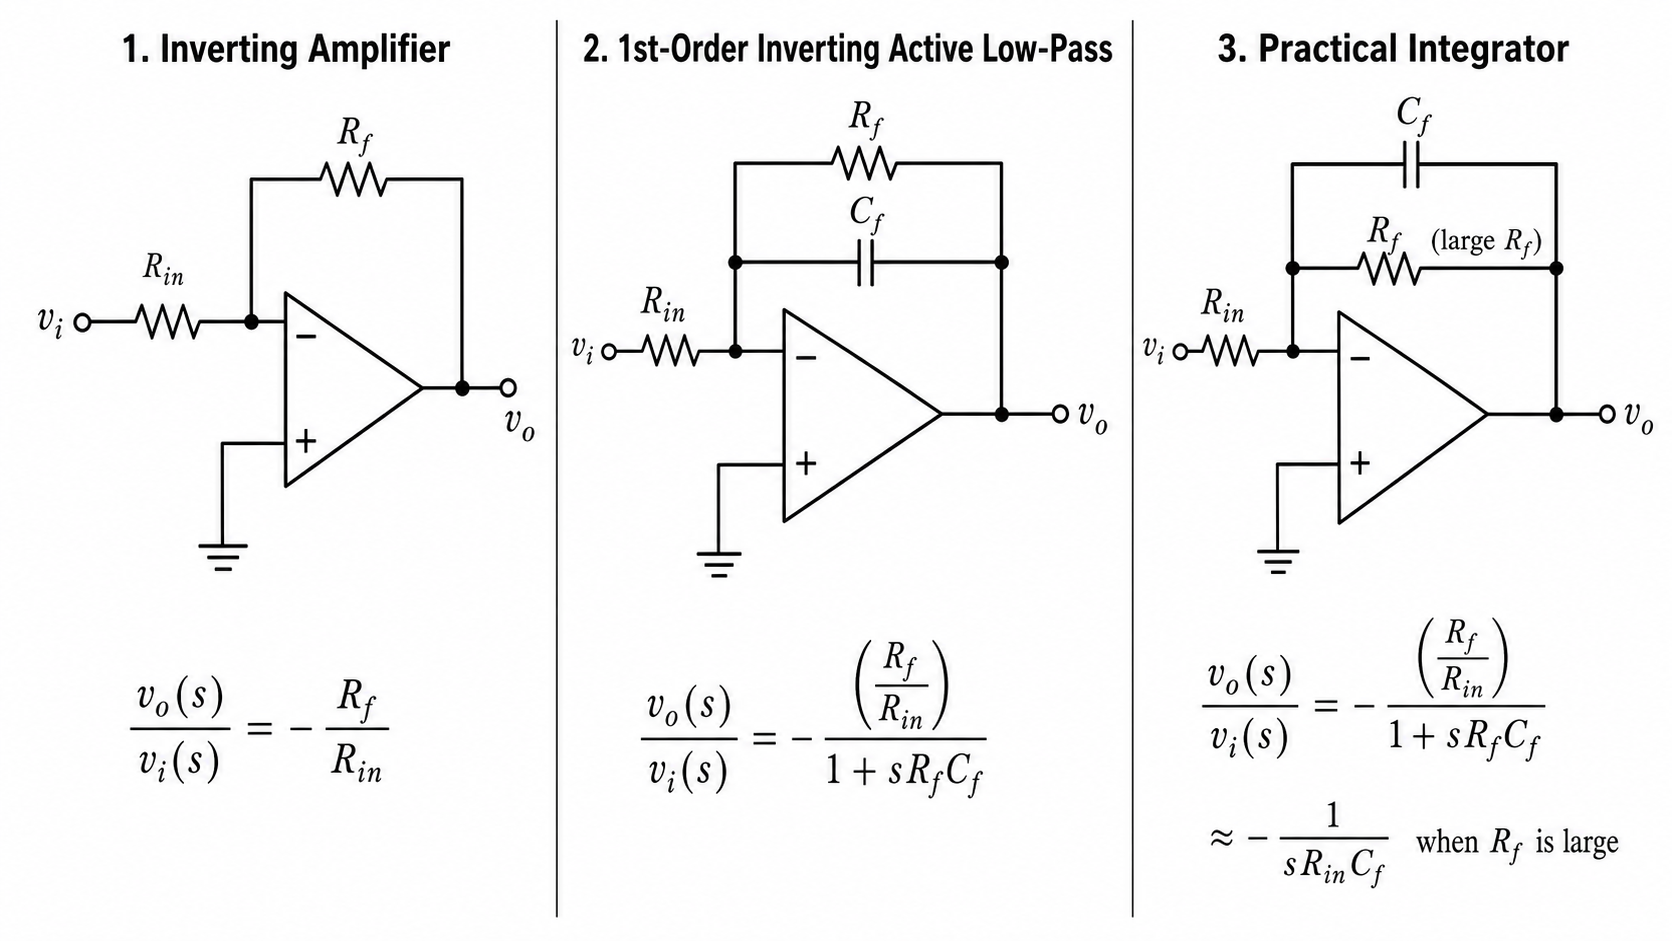
\includegraphics[width=0.8\textwidth]{images/chapter3/figure-6.png}
    \caption{วงจร Op-Amp และฟังก์ชันถ่ายโอน}
\end{figure}

\paragraph{7.5.6 ข้อจำกัดของแบบจำลองวงจรอุดมคติ}

แบบจำลองข้างต้นอาจคลาดเคลื่อนเมื่อ

\begin{itemize}
    \item ตัวต้านทาน ตัวเก็บประจุ และตัวเหนี่ยวนำมีค่าคลาดเคลื่อน
    \item ตัวเหนี่ยวนำมีความต้านทานขดลวดและความจุแฝง
    \item ตัวเก็บประจุมี ESR และการรั่วไหล
    \item เครื่องกำเนิดสัญญาณมีความต้านทานเอาต์พุต
    \item Oscilloscope และหัววัดเพิ่มโหลดให้วงจร
    \item Op-Amp มี gain-bandwidth product, slew rate, input bias current และข้อจำกัดแรงดันเอาต์พุต
    \item ระบบเข้าสู่ช่วงไม่เชิงเส้น เช่น Op-Amp อิ่มตัวหรือแกนอิ่มตัวของตัวเหนี่ยวนำ
\end{itemize}

การเลือกความละเอียดของแบบจำลองจึงต้องสัมพันธ์กับวัตถุประสงค์ หากใช้ศึกษาพฤติกรรมพื้นฐาน แบบจำลองอุดมคติอาจเพียงพอ แต่หากต้องการให้ผลจำลองใกล้ผลทดลอง ต้องรวมพารามิเตอร์แฝงที่สำคัญ

\subsubsection{7.6 การสร้างแบบจำลองระบบไฟฟ้า–กล: มอเตอร์กระแสตรง}

มอเตอร์กระแสตรง (DC Motor) เป็นตัวอย่างสำคัญของระบบไฟฟ้า–กล (University of Michigan, n.d.) เนื่องจากมีการเปลี่ยนพลังงานไฟฟ้าที่ขดลวดอาร์เมเจอร์เป็นแรงบิดและการเคลื่อนที่เชิงหมุน แบบจำลองต้องเชื่อมสมการวงจรไฟฟ้าเข้ากับสมการกลศาสตร์

\paragraph{7.6.1 ตัวแปรและพารามิเตอร์}

\begin{table}[htbp]
    \centering
    \begin{tabular}{l l l}
        \hline
        \textbf{สัญลักษณ์} & \textbf{ความหมาย} & \textbf{หน่วย} \\
        \hline
        $v_a(t)$ & แรงดันอาร์เมเจอร์ & V \\
        $i_a(t)$ & กระแสอาร์เมเจอร์ & A \\
        $R_a$ & ความต้านทานอาร์เมเจอร์ & $\Omega$ \\
        $L_a$ & ความเหนี่ยวนำอาร์เมเจอร์ & H \\
        $e_b(t)$ & แรงดันต้านกลับ (Back EMF) & V \\
        $K_e$ & ค่าคงตัวแรงดันต้านกลับ & V·s/rad \\
        $T_m(t)$ & แรงบิดแม่เหล็กไฟฟ้า & N·m \\
        $K_t$ & ค่าคงตัวแรงบิด & N·m/A \\
        $J$ & โมเมนต์ความเฉื่อยรวมที่เพลา & kg·m$^2$ \\
        $b$ & สัมประสิทธิ์แรงเสียดทานหนืด & N·m·s/rad \\
        $\theta(t)$ & ตำแหน่งเชิงมุม & rad \\
        $\omega(t)=\dot{\theta}(t)$ & ความเร็วเชิงมุม & rad/s \\
        $T_L(t)$ & แรงบิดโหลดรบกวน & N·m \\
        \hline
    \end{tabular}
\end{table}

สำหรับหน่วย SI มักมีค่าตัวเลข $K_t=K_e=K$ แต่มีหน่วยต่างกันและมีความหมายทางกายภาพต่างกัน

\paragraph{7.6.2 สมการส่วนไฟฟ้า}

จาก KVL ที่วงจรอาร์เมเจอร์

\[
v_a(t)=L_a\frac{di_a(t)}{dt}+R_ai_a(t)+e_b(t)
\]

แรงดันต้านกลับแปรผันกับความเร็ว

\[
e_b(t)=K_e\omega(t)
\]

จึงได้

\[
L_a\frac{di_a(t)}{dt}+R_ai_a(t)+K_e\omega(t)=v_a(t)
\]

\paragraph{7.6.3 สมการส่วนกล}

แรงบิดแม่เหล็กไฟฟ้าเป็น

\[
T_m(t)=K_ti_a(t)
\]

สมดุลแรงบิดที่เพลาเมื่อรวมแรงบิดโหลด

\[
J\frac{d\omega(t)}{dt}+b\omega(t)=K_ti_a(t)-T_L(t)
\]

สำหรับการหาฟังก์ชันถ่ายโอนจากแรงดันอาร์เมเจอร์ไปยังความเร็ว ให้กำหนด $T_L(t)=0$

\paragraph{7.6.4 การหาฟังก์ชันถ่ายโอนความเร็ว}

แปลงลาปลาซภายใต้ค่าเริ่มต้นเป็นศูนย์

\[
(L_as+R_a)I_a(s)+K_e\Omega(s)=V_a(s)
\]

\[
(Js+b)\Omega(s)=K_tI_a(s)
\]

จากสมการกล

\[
I_a(s)=\frac{Js+b}{K_t}\Omega(s)
\]

แทนในสมการไฟฟ้า

\[
\left[
\frac{(L_as+R_a)(Js+b)}{K_t}+K_e
\right]\Omega(s)=V_a(s)
\]

จึงได้

\[
\boxed{
\frac{\Omega(s)}{V_a(s)}
=
\frac{K_t}
{(L_as+R_a)(Js+b)+K_tK_e}
}
\]

ขยายพหุนามส่วน

\[
\boxed{
\frac{\Omega(s)}{V_a(s)}
=
\frac{K_t}
{L_aJs^2+(L_ab+R_aJ)s+(R_ab+K_tK_e)}
}
\]

ฟังก์ชันถ่ายโอนตำแหน่งได้จาก $\Omega(s)=s\Theta(s)$

\[
\boxed{
\frac{\Theta(s)}{V_a(s)}
=
\frac{K_t}
{s\left[L_aJs^2+(L_ab+R_aJ)s+(R_ab+K_tK_e)\right]}
}
\]

หากละเลย $L_a$ เพราะค่าคงตัวเวลาทางไฟฟ้า $L_a/R_a$ เล็กกว่าค่าคงตัวเวลาทางกลมาก แบบจำลองความเร็วจะลดเป็นระบบอันดับหนึ่ง

\[
\frac{\Omega(s)}{V_a(s)}
\approx
\frac{K_t}
{R_aJs+(R_ab+K_tK_e)}
\]

อย่างไรก็ตาม การละเลย $L_a$ ต้องอาศัยเหตุผลจากขนาดพารามิเตอร์และช่วงความถี่ที่สนใจ ไม่ควรละเลยโดยอัตโนมัติ

% [รูปที่ 7: แบบจำลองเชื่อมโยงพลังงานของมอเตอร์ DC]
% ประเภทภาพ: Electromechanical Block Diagram / Technical Illustration
% ตำแหน่งที่แนะนำ: หัวข้อ 7.6
% วัตถุประสงค์การเรียนรู้: แสดงการเชื่อมโยงระหว่างแรงดัน กระแส แรงบิด และความเร็ว รวมทั้งป้อนกลับภายในจาก Back EMF
% คำอธิบายภาพ: แผนภาพพลังงานจากแรงดันอาร์เมเจอร์เข้าสู่วงจร $R_a$–$L_a$ ได้กระแส $i_a$ ผ่านค่าคงตัว $K_t$ เป็นแรงบิด ขับระบบกล $1/(Js+b)$ เป็นความเร็ว และความเร็วผ่าน $K_e$ ป้อนกลับลบเป็น Back EMF
% องค์ประกอบที่ต้องมี: จุดรวมสัญญาณ, $V_a(s)$, $I_a(s)$, $K_t$, $T_m(s)$, $1/(Js+b)$, $\Omega(s)$, $K_e$, $E_b(s)$, แรงบิดโหลด $T_L(s)$
% ข้อความหรือป้ายกำกับ: “Armature Circuit”, “Torque Constant”, “Mechanical Dynamics”, “Back EMF”, “Load Torque”
% ภาษาของป้ายกำกับ: อังกฤษ
% สัดส่วนภาพ: 16:9
% Image Generation Prompt: Accurate educational block diagram of an armature-controlled DC motor. Input Va(s) enters a summing junction subtracting back EMF Eb(s), then block 1/(La s + Ra) produces armature current Ia(s). Block Kt produces electromagnetic torque Tm(s). A second summing junction subtracts load torque TL(s), then block 1/(J s + b) produces angular speed Omega(s). Feedback from Omega(s) through Ke returns as Eb(s) to the first summing junction. Blue forward path, orange internal feedback, red disturbance arrow, white background, control engineering textbook style.
% Alt Text: แผนภาพบล็อกมอเตอร์ DC แสดงวงจรอาร์เมเจอร์ การสร้างแรงบิด ระบบกล และแรงดันต้านกลับ

\begin{figure}[htbp]
    \centering
    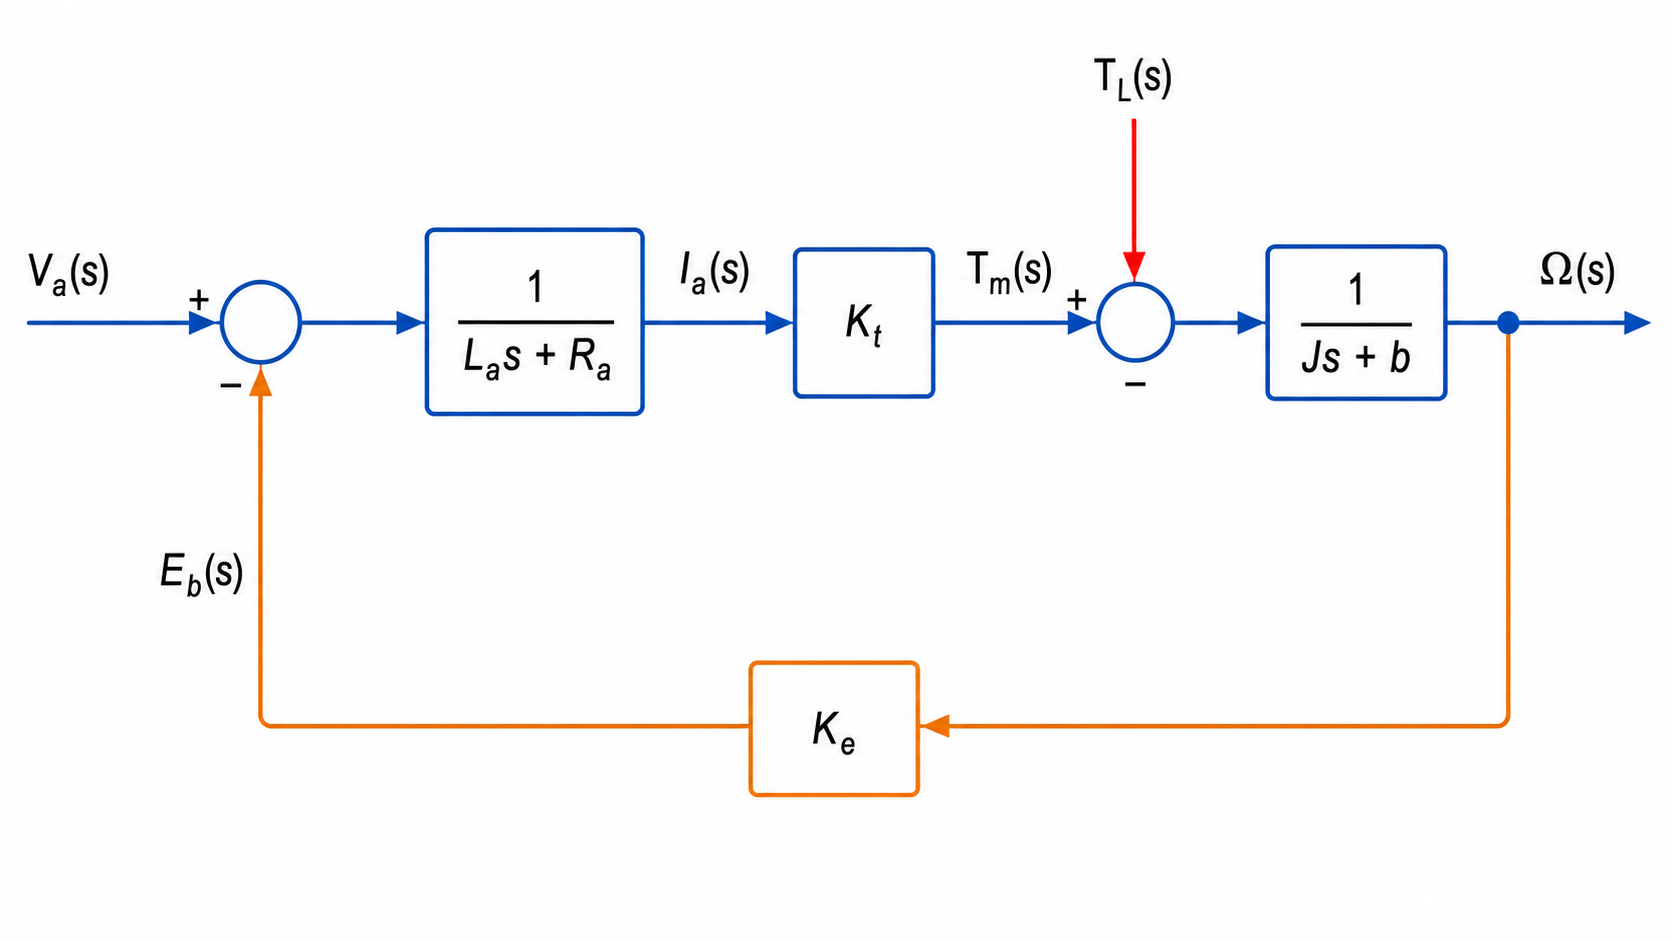
\includegraphics[width=0.8\textwidth]{images/chapter3/figure-7.png}
    \caption{แบบจำลองเชื่อมโยงพลังงานของมอเตอร์ DC}
\end{figure}

\paragraph{7.6.5 ตัวอย่างบังคับ: แบบจำลองมอเตอร์ DC}

\textbf{ตัวอย่างเพิ่มเติมเพื่อการเรียนรู้}\\กำหนด

\[
J=0.01\ \text{kg·m}^2,\quad
b=0.1\ \text{N·m·s/rad}
\]

\[
K_t=K_e=0.01,\quad
R_a=1\ \Omega,\quad
L_a=0.5\ \text{H}
\]

ต้องการฟังก์ชันถ่ายโอนจาก $V_a(s)$ ไปยัง $\Omega(s)$ เมื่อไม่มีแรงบิดโหลดรบกวน

\textbf{1. เลือกสมการทั่วไป}

\[
\frac{\Omega(s)}{V_a(s)}
=
\frac{K_t}
{L_aJs^2+(L_ab+R_aJ)s+(R_ab+K_tK_e)}
\]

\textbf{2. คำนวณสัมประสิทธิ์}

\[
L_aJ=(0.5)(0.01)=0.005
\]

\[
L_ab+R_aJ=(0.5)(0.1)+(1)(0.01)=0.06
\]

\[
R_ab+K_tK_e=(1)(0.1)+(0.01)(0.01)=0.1001
\]

\textbf{3. เขียนฟังก์ชันถ่ายโอน}

\[
\boxed{
\frac{\Omega(s)}{V_a(s)}
=
\frac{0.01}{0.005s^2+0.06s+0.1001}
}
\]

หารทั้งเศษและส่วนด้วย $0.005$

\[
\boxed{
\frac{\Omega(s)}{V_a(s)}
=
\frac{2}{s^2+12s+20.02}
}
\]

\textbf{4. วิเคราะห์โพล}

รากของส่วนมีค่าประมาณ

\[
p_1\approx-2.0025,\qquad
p_2\approx-9.9975
\]

โพลทั้งสองอยู่ซีกซ้ายของระนาบเชิงซ้อน จึงเป็นแบบจำลองที่เสถียร โพลที่อยู่ใกล้จุดกำเนิดกว่าคือ $p_1$ มีอิทธิพลต่อพฤติกรรมช้ามากกว่า

\textbf{5. ตรวจสอบอัตราขยายสภาวะคงตัว}

\[
G(0)=\frac{0.01}{0.1001}
\approx0.0999\ \frac{\text{rad/s}}{\text{V}}
\]

หากป้อนแรงดันคงที่ $10\ \text{V}$ แบบจำลองทำนายความเร็วสภาวะคงตัวประมาณ

\[
\omega_{ss}\approx0.999\ \text{rad/s}
\]

ค่าตัวเลขตัวอย่างนี้ใช้เพื่อฝึกกระบวนการสร้างแบบจำลอง ไม่ได้แทนมอเตอร์ชนิดใดโดยเฉพาะ

\paragraph{7.6.6 แบบจำลองที่มีแรงบิดโหลดเป็นอินพุตรบกวน}

เมื่อเก็บ $T_L(s)$ ไว้ จะได้ระบบสองอินพุต

\[
\Omega(s)
=
G_v(s)V_a(s)+G_d(s)T_L(s)
\]

โดย

\[
G_v(s)=
\frac{K_t}
{(L_as+R_a)(Js+b)+K_tK_e}
\]

และ

\[
G_d(s)=
-\frac{L_as+R_a}
{(L_as+R_a)(Js+b)+K_tK_e}
\]

เครื่องหมายลบแสดงว่าแรงบิดโหลดที่ต้านการหมุนทำให้ความเร็วลดลง การแยกเส้นทางอินพุตควบคุมและอินพุตรบกวนมีประโยชน์ต่อการวิเคราะห์ระบบควบคุมในบทถัดไป

\par\noindent\rule{\textwidth}{0.4pt}\par

\subsubsection{7.7 การเขียนสมการสถานะเบื้องต้นจาก Transfer Function}

ฟังก์ชันถ่ายโอนอธิบายความสัมพันธ์อินพุต–เอาต์พุต แต่ไม่แสดงตัวแปรภายในโดยตรง แบบจำลองปริภูมิสถานะ (State-Space Model) เขียนในรูป

\[
\dot{\mathbf{x}}(t)=A\mathbf{x}(t)+B\mathbf{u}(t)
\]

\[
\mathbf{y}(t)=C\mathbf{x}(t)+D\mathbf{u}(t)
\]

โดย

\begin{itemize}
    \item $\mathbf{x}(t)$ คือเวกเตอร์สถานะ
    \item $\mathbf{u}(t)$ คือเวกเตอร์อินพุต
    \item $\mathbf{y}(t)$ คือเวกเตอร์เอาต์พุต
    \item $A$ คือเมทริกซ์พลวัตของระบบ
    \item $B$ คือเมทริกซ์อินพุต
    \item $C$ คือเมทริกซ์เอาต์พุต
    \item $D$ คือเมทริกซ์ส่งผ่านโดยตรง
\end{itemize}

สำหรับระบบ LTI ที่มีค่าเริ่มต้นเป็นศูนย์ ความสัมพันธ์กับฟังก์ชันถ่ายโอนคือ

\[
\boxed{
G(s)=C(sI-A)^{-1}B+D
}
\]

แบบจำลองสถานะของฟังก์ชันถ่ายโอนหนึ่งชุด \textbf{ไม่เป็นเอกลักษณ์} (Massachusetts Institute of Technology OpenCourseWare, n.d.) กล่าวคือ มีเมทริกซ์ $A,B,C,D$ ได้หลายชุดที่ให้ความสัมพันธ์อินพุต–เอาต์พุตเดียวกัน หากสถานะถูกแปลงด้วยเมทริกซ์ไม่เอกฐาน ระบบใหม่ยังคงมีฟังก์ชันถ่ายโอนเดิม

\paragraph{7.7.1 รูป Canonical สำหรับระบบอันดับสอง}

ให้

\[
G(s)=\frac{b_1s+b_0}{s^2+a_1s+a_0}
\]

รูป Controllable Canonical Form หนึ่งรูปคือ

\[
A=
\begin{bmatrix}
0 & 1\\
-a_0 & -a_1
\end{bmatrix},
\qquad
B=
\begin{bmatrix}
0\\
1
\end{bmatrix}
\]

\[
C=
\begin{bmatrix}
b_0 & b_1
\end{bmatrix},
\qquad
D=0
\]

ตรวจสอบได้จาก $G(s)=C(sI-A)^{-1}B$

หากเศษมีดีกรีเท่ากับส่วน ต้องแยกพจน์ส่งผ่านโดยตรง $D$ ก่อน เพื่อให้ส่วนที่เหลือเป็นฟังก์ชันถ่ายโอน proper

\paragraph{7.7.2 ตัวอย่าง: แปลง Transfer Function ของระบบกลเป็น State Equation}

จากตัวอย่างระบบมวล–สปริง–ตัวหน่วง

\[
G(s)=\frac{X(s)}{F(s)}
=\frac{1}{2s^2+6s+8}
=\frac{0.5}{s^2+3s+4}
\]

ดังนั้น

\[
a_1=3,\quad a_0=4,\quad b_1=0,\quad b_0=0.5
\]

รูป Canonical คือ

\[
A=
\begin{bmatrix}
0 & 1\\
-4 & -3
\end{bmatrix},
\quad
B=
\begin{bmatrix}
0\\
1
\end{bmatrix}
\]

\[
C=
\begin{bmatrix}
0.5 & 0
\end{bmatrix},
\quad
D=0
\]

อีกวิธีหนึ่งคือเลือกสถานะทางกายภาพ

\[
x_1=x,\qquad x_2=\dot{x}
\]

จาก

\[
2\ddot{x}+6\dot{x}+8x=F
\]

จะได้

\[
\dot{x}_1=x_2
\]

\[
\dot{x}_2=-4x_1-3x_2+0.5F
\]

ดังนั้น

\[
A=
\begin{bmatrix}
0 & 1\\
-4 & -3
\end{bmatrix},
\quad
B=
\begin{bmatrix}
0\\
0.5
\end{bmatrix}
\]

\[
C=
\begin{bmatrix}
1 & 0
\end{bmatrix},
\quad
D=0
\]

ทั้งสอง realization ให้ฟังก์ชันถ่ายโอนเดียวกัน แต่ความหมายของสถานะต่างกัน รูปที่ใช้สถานะทางกายภาพมักตีความได้ง่ายกว่า ส่วนรูป canonical สร้างจากสัมประสิทธิ์พหุนามได้โดยตรง

% [รูปที่ 8: เปรียบเทียบ Transfer Function และ State-Space Realization]
% ประเภทภาพ: Conceptual Block Diagram
% ตำแหน่งที่แนะนำ: หัวข้อ 7.7
% วัตถุประสงค์การเรียนรู้: แสดงว่าฟังก์ชันถ่ายโอนเดียวกันสามารถมีการเลือกสถานะหลายแบบ
% คำอธิบายภาพ: ด้านซ้ายเป็นกล่อง $G(s)$ เชื่อมอินพุต $u$ กับเอาต์พุต $y$ ด้านขวาแตกแขนงเป็น realization สองแบบ ได้แก่ canonical states และ physical states โดยลูกศรทั้งสองย้อนกลับมาที่ฟังก์ชันถ่ายโอนเดียวกัน
% องค์ประกอบที่ต้องมี: $u(t)$, $y(t)$, $G(s)$, $A,B,C,D$, canonical states, physical states, ลูกศร similarity transformation
% ข้อความหรือป้ายกำกับ: “Input–Output Model”, “Internal-State Model”, “Non-unique Realizations”, “Same Transfer Function”
% ภาษาของป้ายกำกับ: อังกฤษ
% สัดส่วนภาพ: 16:9
% Image Generation Prompt: Educational control-systems diagram comparing a transfer-function input-output model with two state-space realizations. Left: u(t) enters a block G(s) and produces y(t). Right: two parallel boxes labeled Controllable Canonical States and Physical States, each containing A, B, C, D matrices; arrows indicate both produce the same G(s), with a similarity transformation arrow between the realizations. Clean academic vector style, white background, blue and gray accents.
% Alt Text: ฟังก์ชันถ่ายโอนหนึ่งชุดเชื่อมโยงกับแบบจำลองสถานะได้หลายรูปแบบที่ให้ผลอินพุต–เอาต์พุตเดียวกัน

\begin{figure}[htbp]
    \centering
    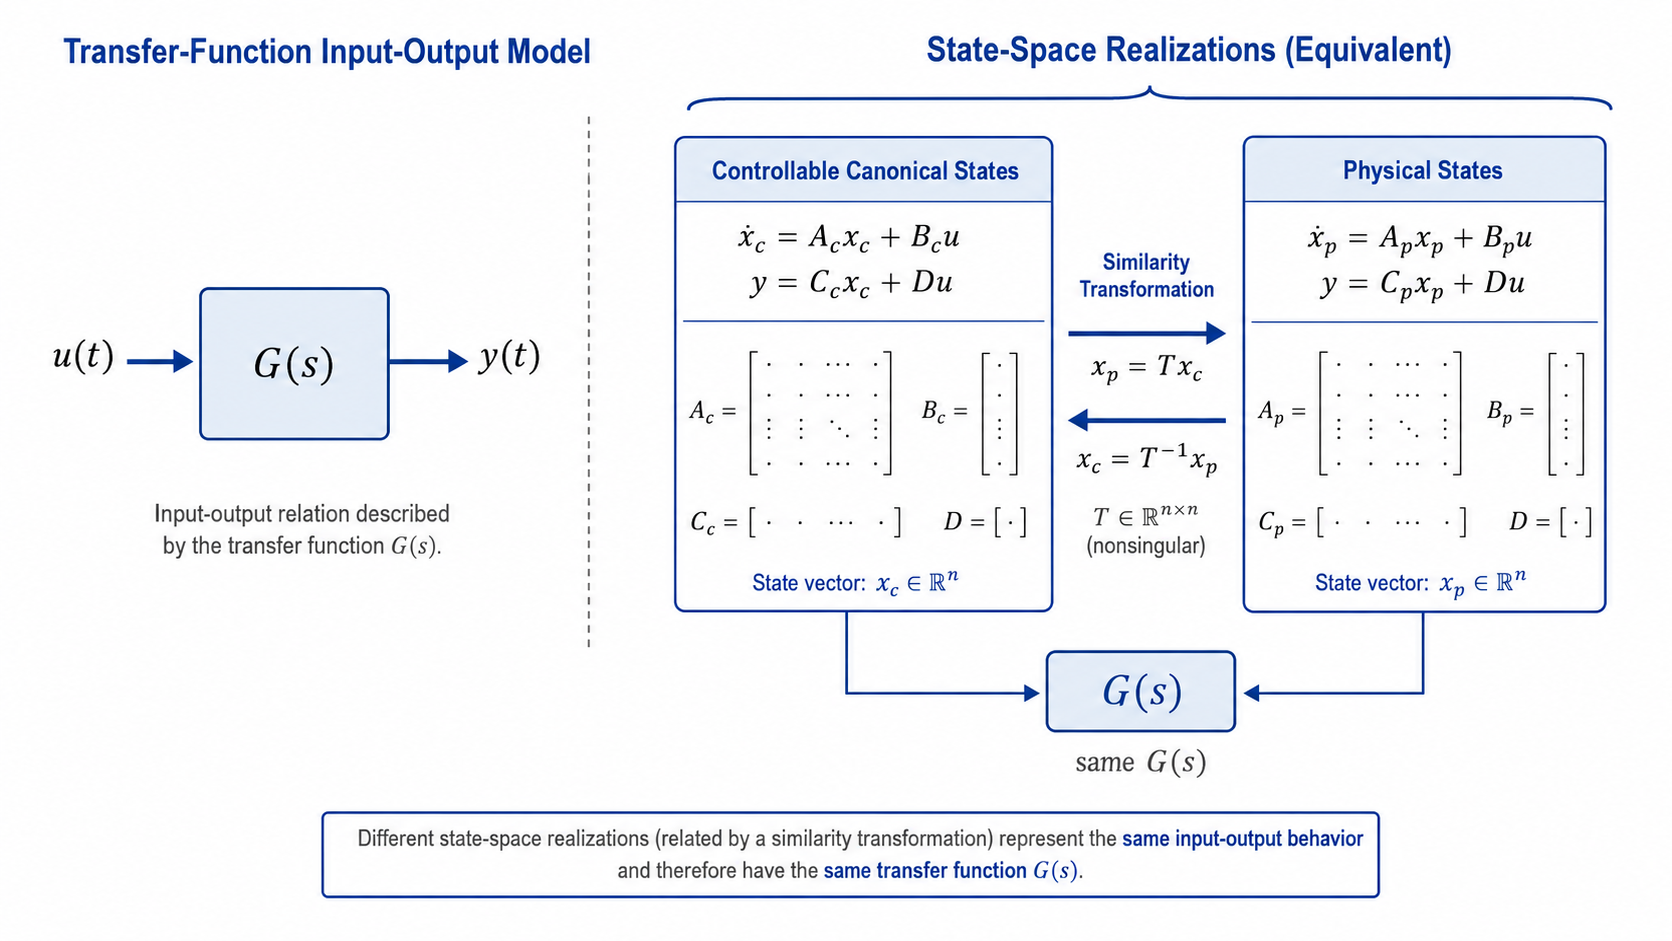
\includegraphics[width=0.8\textwidth]{images/chapter3/figure-8.png}
    \caption{เปรียบเทียบ Transfer Function และ State-Space Realization}
\end{figure}

\par\noindent\rule{\textwidth}{0.4pt}\par

\subsubsection{7.8 การตรวจสอบและยืนยันแบบจำลอง}

การได้สมการไม่ใช่จุดสิ้นสุดของการสร้างแบบจำลอง ควรตรวจสอบอย่างน้อยสี่ระดับ

\paragraph{7.8.1 ตรวจสอบโครงสร้างและหน่วย}

\begin{itemize}
    \item สมการทุกพจน์ต้องมีหน่วยเดียวกัน
    \item อันดับของระบบควรสัมพันธ์กับจำนวนองค์ประกอบสะสมพลังงานอิสระ
    \item เครื่องหมายของแรง แรงบิด แรงดัน และกระแสต้องสอดคล้องกับทิศทางอ้างอิง
    \item ฟังก์ชันถ่ายโอนของระบบกายภาพทั่วไปควรเป็น proper เว้นแต่มีเหตุผลเฉพาะ
\end{itemize}

\paragraph{7.8.2 ตรวจสอบกรณีขอบเขต}

ตัวอย่างเช่น

\begin{itemize}
    \item $s\rightarrow0$ แสดงพฤติกรรมสภาวะคงตัว
    \item $s\rightarrow\infty$ แสดงแนวโน้มความถี่สูง
    \item $R\rightarrow0$, $C\rightarrow0$, $m\rightarrow0$ หรือพารามิเตอร์อื่นควรให้พฤติกรรมที่มีเหตุผล
    \item เมื่อไม่มีการหน่วง ระบบควรสะท้อนการสั่นตามธรรมชาติที่เหมาะสม
\end{itemize}

\paragraph{7.8.3 ตรวจสอบด้วยการจำลอง}

เปรียบเทียบ

\begin{enumerate}
    \item ผลจากสมการเชิงอนุพันธ์
    \item ผลจาก Transfer Function
    \item ผลจาก State-Space
    \item ผลจาก Simulink
\end{enumerate}

สำหรับอินพุตและค่าเริ่มต้นเดียวกัน ผลควรสอดคล้องกันภายในความคลาดเคลื่อนเชิงตัวเลข

\paragraph{7.8.4 ตรวจสอบกับข้อมูลทดลอง}

ใช้ตัวชี้วัด เช่น

\[
\%\text{Error}
=
\left|
\frac{x_{\text{measured}}-x_{\text{model}}}
{x_{\text{model}}}
\right|\times100
\]

สำหรับข้อมูลหลายจุด อาจใช้ค่าเฉลี่ยความคลาดเคลื่อนสัมบูรณ์

\[
\text{MAE}
=
\frac{1}{N}\sum_{k=1}^{N}
|y_k-\hat{y}_k|
\]

ความคลาดเคลื่อนไม่ได้หมายความว่าแบบจำลอง “ผิด” เสมอไป แต่อาจบ่งชี้ว่า

\begin{itemize}
    \item พารามิเตอร์จริงต่างจากค่าป้ายกำกับ
    \item มีไดนามิกที่ละเลย
    \item เครื่องมือวัดและการสุ่มตัวอย่างมีข้อจำกัด
    \item ระบบมีสัญญาณรบกวนหรือไม่เชิงเส้น
    \item จุดทำงานของระบบเปลี่ยนไป
\end{itemize}

\par\noindent\rule{\textwidth}{0.4pt}\par

\subsection{8. การใช้ MATLAB และ Simulink เพื่อสร้างและตรวจสอบแบบจำลอง}

\subsubsection{8.1 วัตถุประสงค์}

หลังจากศึกษาส่วนนี้ นักศึกษาควรสามารถ

\begin{enumerate}
    \item สร้างวัตถุ Transfer Function จากสัมประสิทธิ์เศษและส่วน
    \item ตรวจสอบโพล ซีโร และการตอบสนองขั้นบันได
    \item แปลง Transfer Function เป็น State-Space
    \item สร้างแบบจำลองบล็อกใน Simulink
    \item เปรียบเทียบผลคำนวณ ผลจำลอง และผลทดลอง
\end{enumerate}

\begin{quote}
\textbf{หมายเหตุด้านเวอร์ชัน:} ชื่อคำสั่งและบล็อกต่อไปนี้เป็นชื่อมาตรฐานที่ใช้ทั่วไปใน MATLAB/Simulink แต่หน้าตาเมนูอาจแตกต่างตามเวอร์ชันและผลิตภัณฑ์เสริมที่ติดตั้ง
\end{quote}

\subsubsection{8.2 MATLAB: ระบบมวล–สปริง–ตัวหน่วง}

\begin{verbatim}
% Mass-spring-damper parameters
m = 2;      % kg
c = 6;      % N*s/m
k = 8;      % N/m

% G(s) = X(s)/F(s)
num_msd = 1;
den_msd = [m c k];
G_msd = tf(num_msd, den_msd);

disp(G_msd)
pole(G_msd)
zero(G_msd)

figure
step(G_msd)
grid on
title('Step response: Mass-Spring-Damper')
xlabel('Time (s)')
ylabel('Displacement (m) for 1-N step force')
\end{verbatim}

\textbf{สิ่งที่ควรสังเกต}

\begin{itemize}
    \item สัมประสิทธิ์ใน \texttt{den\_msd} เรียงตามกำลังของ $s$ จากมากไปน้อย
    \item การตอบสนองต่อแรงขั้นบันไดขนาด $1\ \text{N}$ ควรเข้าสู่ $1/k=0.125\ \text{m}$
    \item โพลต้องตรงกับรากของ $2s^2+6s+8$
\end{itemize}

\subsubsection{8.3 MATLAB: วงจร RLC}

\begin{verbatim}
R = 100;        % ohm
L = 10e-3;      % H
C = 1e-6;       % F

% G(s) = Vc(s)/Vin(s)
num_rlc = 1;
den_rlc = [L*C R*C 1];
G_rlc = tf(num_rlc, den_rlc);

figure
step(G_rlc)
grid on
title('Step response: Series RLC, output across C')
xlabel('Time (s)')
ylabel('Normalized capacitor voltage')

figure
bode(G_rlc)
grid on
\end{verbatim}

สำหรับแบบจำลองเชิงปฏิบัติ ให้แทน \texttt{R} ด้วย $R_{\text{eq}}$ ที่รวมความต้านทานแหล่งกำเนิดและขดลวด

\begin{verbatim}
Rs = 50;        % source resistance, ohm
rL = 20;        % measured inductor winding resistance, ohm
Req = R + Rs + rL;

G_rlc_practical = tf(1, [L*C Req*C 1]);

figure
bode(G_rlc, G_rlc_practical)
grid on
legend('Ideal', 'Practical')
\end{verbatim}

\subsubsection{8.4 MATLAB: มอเตอร์ DC}

\begin{verbatim}
J  = 0.01;      % kg*m^2
b  = 0.1;       % N*m*s/rad
Kt = 0.01;      % N*m/A
Ke = 0.01;      % V*s/rad
Ra = 1;         % ohm
La = 0.5;       % H

num_motor = Kt;
den_motor = [La*J, La*b + Ra*J, Ra*b + Kt*Ke];

G_motor = tf(num_motor, den_motor);

disp(G_motor)
pole(G_motor)
dcgain(G_motor)

figure
step(G_motor)
grid on
title('DC Motor Speed Response')
xlabel('Time (s)')
ylabel('Angular speed (rad/s) for 1-V step')
\end{verbatim}

\subsubsection{8.5 แปลง Transfer Function เป็น State-Space}

\begin{verbatim}
[A, B, Cmat, D] = tf2ss(num_msd, den_msd);

disp(A)
disp(B)
disp(Cmat)
disp(D)

sys_ss = ss(A, B, Cmat, D);

figure
step(G_msd, sys_ss)
grid on
legend('Transfer Function', 'State Space')
title('Comparison of equivalent realizations')
\end{verbatim}

ผลการตอบสนองอินพุต–เอาต์พุตควรซ้อนกัน แต่ค่าของสถานะภายในอาจไม่ตรงกับตำแหน่งและความเร็วทางกายภาพ เนื่องจาก \texttt{tf2ss} สร้าง realization ตามรูปแบบเชิงคำนวณ

\subsubsection{8.6 การสร้างแบบจำลองใน Simulink}

\paragraph{8.6.1 บล็อกที่ใช้}

\begin{itemize}
    \item \textbf{Step}: สร้างอินพุตขั้นบันได
    \item \textbf{Transfer Fcn}: ป้อนสัมประสิทธิ์เศษและส่วน
    \item \textbf{Scope}: แสดงสัญญาณเวลา
    \item \textbf{To Workspace}: ส่งข้อมูลไปวิเคราะห์ใน MATLAB
    \item \textbf{Mux}: รวมสัญญาณเพื่อเปรียบเทียบ
    \item \textbf{Sum}, \textbf{Gain}, \textbf{Integrator}: ใช้สร้างแบบจำลองจากสมการสถานะหรือสมการเชิงอนุพันธ์
\end{itemize}

\paragraph{8.6.2 แบบจำลอง RLC ด้วย Transfer Fcn}

\begin{enumerate}
    \item วางบล็อก \texttt{Step}
    \item ต่อเข้าบล็อก \texttt{Transfer Fcn}
    \item กำหนด Numerator เป็น \texttt{[1]}
    \item กำหนด Denominator เป็น \texttt{[L*C R*C 1]} หรือใส่ค่าตัวเลข \texttt{[1e-8 1e-4 1]}
    \item ต่อเอาต์พุตเข้าบล็อก \texttt{Scope}
    \item กำหนด Stop Time ให้ครอบคลุมหลายคาบของพลวัต เช่น \texttt{0.005} s
    \item รันแบบจำลองและอ่านค่า overshoot, rise time และ settling behavior
\end{enumerate}

\paragraph{8.6.3 แบบจำลอง RLC จาก Integrator}

จาก

\[
LC\ddot{v}_o+RC\dot{v}_o+v_o=v_i
\]

จัดรูป

\[
\ddot{v}_o
=
\frac{1}{LC}v_i
-\frac{R}{L}\dot{v}_o
-\frac{1}{LC}v_o
\]

ใช้ Integrator สองตัวต่ออนุกรมเพื่อสร้าง $\dot{v}_o$ และ $v_o$ แล้วป้อนกลับทั้งสองสัญญาณผ่าน Gain ที่เหมาะสม วิธีนี้ทำให้เห็นโครงสร้างสถานะของระบบโดยตรง

% [รูปที่ 9: แบบจำลอง Simulink ของวงจร RLC สองแนวทาง]
% ประเภทภาพ: Software Block Diagram
% ตำแหน่งที่แนะนำ: หัวข้อ 8.6
% วัตถุประสงค์การเรียนรู้: เปรียบเทียบการจำลองด้วยบล็อก Transfer Fcn กับการสร้างจากสมการเชิงอนุพันธ์
% คำอธิบายภาพ: ด้านบนเป็น Step → Transfer Fcn → Scope ด้านล่างเป็น Sum ต่อ Integrator สองตัว พร้อม Gain ป้อนกลับจาก $v_o$ และ $\dot{v}_o$ โดยเอาต์พุตทั้งสองแนวทางเข้า Mux และ Scope เดียวกัน
% องค์ประกอบที่ต้องมี: Step, Transfer Fcn, Sum, Gain, Integrator สองตัว, Mux, Scope, ป้าย $v_i$, $\dot{v}_o$, $v_o$
% ข้อความหรือป้ายกำกับ: “Transfer-Function Model”, “Differential-Equation Model”, “Compare Outputs”
% ภาษาของป้ายกำกับ: อังกฤษ
% สัดส่วนภาพ: 16:9
% Image Generation Prompt: MATLAB Simulink-style educational block diagram comparing two equivalent series RLC models. Top path: Step block to Transfer Fcn block with numerator [1] and denominator [LC RC 1], then Scope. Bottom path: Step enters a summing block that also receives negative feedback from vo and vo-dot through gains; output drives two cascaded Integrator blocks to produce vo-dot and vo. Feed both model outputs through a Mux into one Scope. Use authentic generic block-diagram appearance without software logos, clear signal labels, white canvas.
% Alt Text: แบบจำลอง RLC ใน Simulink โดยใช้ Transfer Fcn และ Integrator สองตัวเพื่อเปรียบเทียบผล

\begin{figure}[htbp]
    \centering
    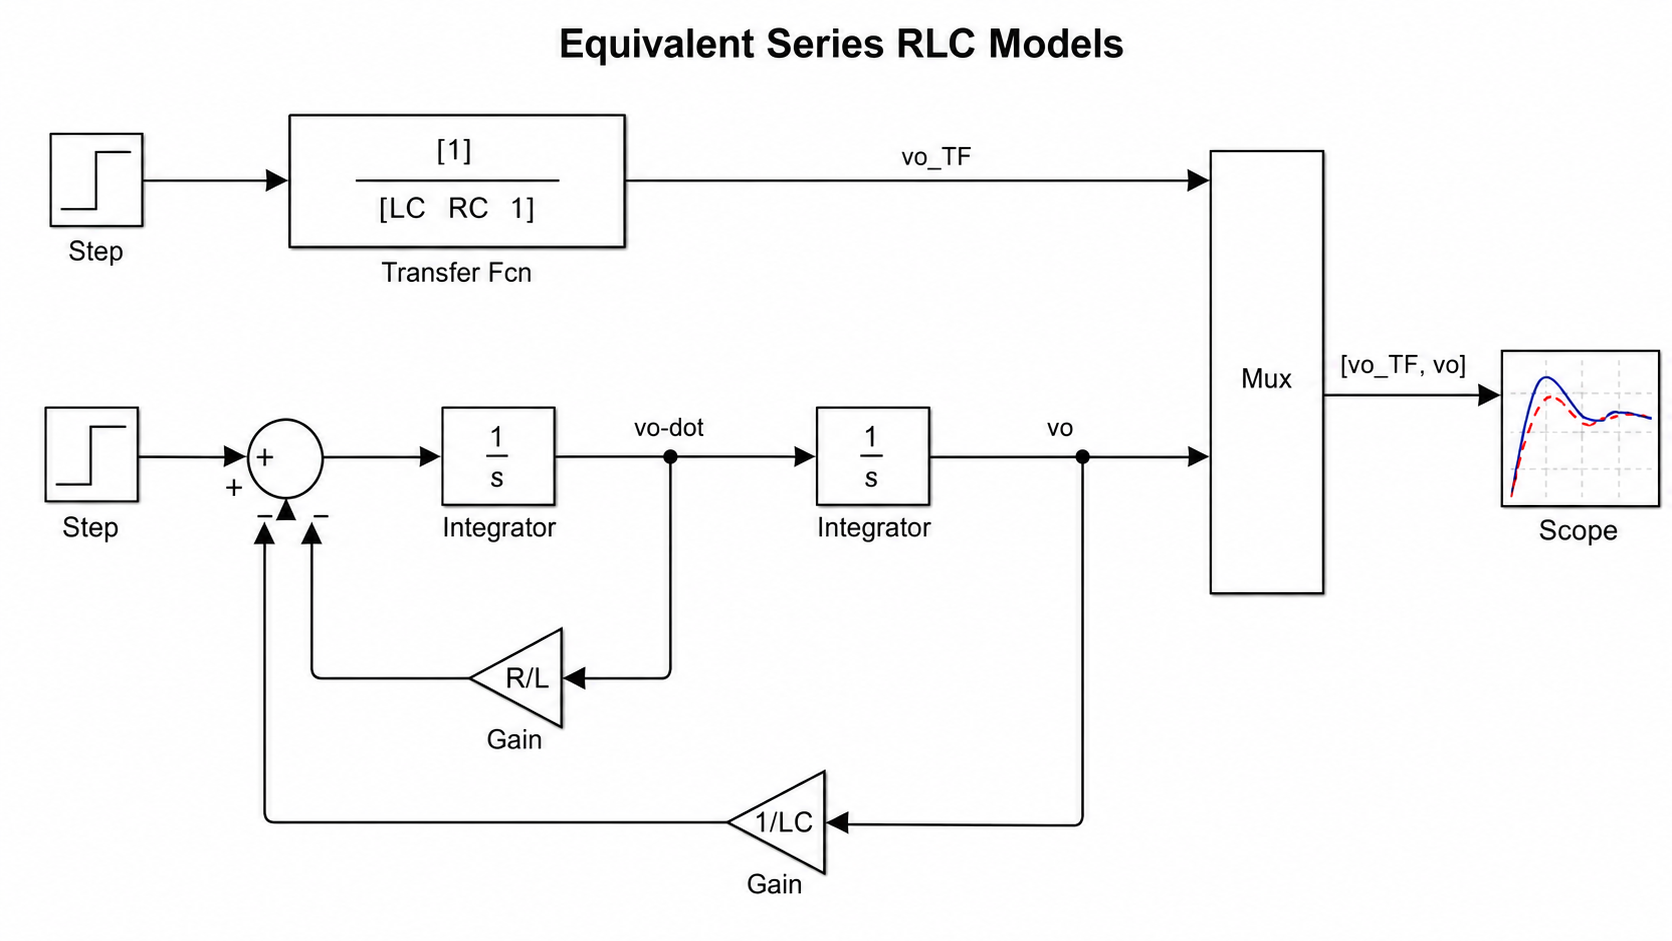
\includegraphics[width=0.8\textwidth]{images/chapter3/figure-9.png}
    \caption{แบบจำลอง Simulink ของวงจร RLC สองแนวทาง}
\end{figure}

\subsubsection{8.7 ผลลัพธ์ที่คาดหวังและวิธีอ่านผล}

\begin{itemize}
    \item กราฟ RLC จากสองแบบจำลองควรซ้อนกันเมื่อใช้พารามิเตอร์และค่าเริ่มต้นเดียวกัน
    \item แบบจำลองอุดมคติที่ $\zeta=0.5$ ควรมีการสั่นและ overshoot ก่อนเข้าสู่ค่าสภาวะคงตัว
    \item เมื่อเพิ่ม $R_{\text{eq}}$ การหน่วงเพิ่ม ยอดเรโซแนนซ์และ overshoot ลดลง
    \item การตอบสนองของมอเตอร์ต้องเข้าสู่ค่า \texttt{dcgain(G\_motor)} สำหรับอินพุตขั้นบันไดหนึ่งหน่วย
    \item หากผลไม่ตรง ให้ตรวจสอบลำดับสัมประสิทธิ์ หน่วย และตำแหน่งเอาต์พุต
\end{itemize}

\subsubsection{8.8 ข้อผิดพลาดที่พบบ่อยในการใช้ซอฟต์แวร์}

\begin{table}[htbp]
    \centering
    \begin{tabular}{l l l}
        \hline
        \textbf{ข้อผิดพลาด} & \textbf{อาการ} & \textbf{วิธีตรวจสอบ} \\
        \hline
        เรียงสัมประสิทธิ์ผิด & โพลและรูปกราฟผิดอย่างมาก & เขียนพหุนามเต็มก่อนสร้างเวกเตอร์ \\
        ใช้ mH หรือ $\mu$F โดยไม่แปลง SI & เวลาตอบสนองผิดหลายลำดับขนาด & แปลงเป็น H และ F \\
        ใส่ \texttt{[1 R*C L*C]} แทน \texttt{[L*C R*C 1]} & แบบจำลองไม่ตรงสมการ & ตรวจลำดับ $s^2,s,1$ \\
        Stop Time สั้นเกินไป & เห็นเฉพาะช่วงต้น & ประมาณจาก $1/|\operatorname{Re}(p)|$ \\
        Solver step ใหญ่เกินไป & กราฟหยาบหรือคลาดเคลื่อน & ลด Max Step Size \\
        ค่าเริ่มต้นของ Integrator ไม่ตรงกัน & TF และ integrator model ไม่ซ้อนกัน & กำหนด initial condition ให้สอดคล้อง \\
        ใช้ Transfer Fcn กับค่าเริ่มต้นไม่เป็นศูนย์โดยไม่พิจารณา & ผลไม่ตรงระบบจริง & ใช้ State-Space หรือ integrator realization \\
        \hline
    \end{tabular}
\end{table}

\subsubsection{8.9 ข้อจำกัดของการจำลอง}

ซอฟต์แวร์คำนวณตามแบบจำลองที่ผู้ใช้กำหนด จึงไม่สามารถชดเชยสมมติฐานที่ไม่เหมาะสมได้เอง ผลจำลองที่ดูเรียบร้อยอาจยังไม่แทนระบบจริง หากละเลยพารามิเตอร์แฝง ความอิ่มตัว สัญญาณรบกวน ความล่าช้า หรือข้อจำกัดเครื่องมือวัด การจำลองควรใช้ร่วมกับการตรวจสอบหน่วย การวิเคราะห์เชิงกายภาพ และข้อมูลทดลอง

\subsection{9. กิจกรรมปฏิบัติการ: การสร้างและตรวจสอบแบบจำลองวงจร RLC}

\subsection{กิจกรรมปฏิบัติการที่ 1: การเปรียบเทียบวงจร RLC จริงกับ Transfer Function และ Simulink}

\subsubsection{9.1 วัตถุประสงค์}

เมื่อเสร็จสิ้นกิจกรรม นักศึกษาสามารถ

\begin{enumerate}
    \item ต่อวงจร RLC อนุกรมบนเบรดบอร์ดได้ถูกต้องและปลอดภัย
    \item วัดแอมพลิจูดและความต่างเฟสของสัญญาณด้วย Oscilloscope
    \item สร้างสมการเชิงอนุพันธ์และ Transfer Function ของวงจร
    \item ประมาณค่าพารามิเตอร์แฝงที่มีผลต่อการตอบสนอง
    \item สร้างแบบจำลองวงจรใน MATLAB/Simulink
    \item เปรียบเทียบผลทฤษฎี ผลจำลอง และผลทดลอง พร้อมอภิปรายความคลาดเคลื่อน
\end{enumerate}

\subsubsection{9.2 หลักการและทฤษฎีที่เกี่ยวข้อง}

วงจร RLC อนุกรมที่วัดเอาต์พุตคร่อมตัวเก็บประจุมีแบบจำลองอุดมคติ และสามารถใช้ศึกษาความถี่เรโซแนนซ์และแบนด์วิดท์ได้ (Analog Devices, n.d.)

\[
G(s)=\frac{V_o(s)}{V_i(s)}
=\frac{1}{LCs^2+RCs+1}
\]

สำหรับแบบจำลองเชิงปฏิบัติ

\[
G_p(s)
=
\frac{1}
{LCs^2+R_{\text{eq}}Cs+1}
\]

โดย

\[
R_{\text{eq}}=R+R_s+r_L+r_{\text{wire}}
\]

เมื่อแทน $s=j\omega$

\[
G(j\omega)
=
\frac{1}
{1-LC\omega^2+jR_{\text{eq}}C\omega}
\]

ขนาดอัตราขยายคือ

\[
|G(j\omega)|
=
\frac{1}
{\sqrt{(1-LC\omega^2)^2+(R_{\text{eq}}C\omega)^2}}
\]

และมุมเฟสคือ

\[
\angle G(j\omega)
=
-\tan^{-1}
\left(
\frac{R_{\text{eq}}C\omega}
{1-LC\omega^2}
\right)
\]

ในการคำนวณมุมควรใช้ฟังก์ชันแบบ \texttt{atan2} เพื่อรักษาควอดแรนต์ให้ถูกต้อง

อัตราขยายจากค่าที่วัดได้

\[
M_{\text{meas}}=\frac{V_{o,\text{pp}}}{V_{i,\text{pp}}}
\]

การแปลงเป็นเดซิเบล

\[
M_{\text{dB}}=20\log_{10}(M_{\text{meas}})
\]

หากวัดความต่างเวลาระหว่างสัญญาณ $\Delta t$ ที่ความถี่ $f$

\[
\phi=360^\circ f\Delta t
\]

ต้องกำหนดเครื่องหมายตามว่าสัญญาณเอาต์พุตนำหรือล้าหลังอินพุต

\subsubsection{9.3 อุปกรณ์ เครื่องมือ และซอฟต์แวร์}

\begin{table}[htbp]
    \centering
    \begin{tabular}{l r l}
        \hline
        \textbf{รายการ} & \textbf{จำนวนต่อกลุ่ม} & \textbf{ข้อกำหนดแนะนำ} \\
        \hline
        เบรดบอร์ด & 1 & สภาพสมบูรณ์ \\
        ตัวต้านทาน & 1–2 & $100\ \Omega$, กำลังอย่างน้อย $0.25\ \text{W}$ \\
        ตัวเหนี่ยวนำ & 1 & ประมาณ $10\ \text{mH}$ และวัด $r_L$ ได้ \\
        ตัวเก็บประจุ & 1 & ประมาณ $1\ \mu\text{F}$ ชนิดเหมาะกับสัญญาณ AC \\
        Function Generator & 1 & sine wave, เอาต์พุตแรงดันต่ำ \\
        Digital Oscilloscope & 1 & อย่างน้อย 2 ช่องสัญญาณ \\
        หัววัด Oscilloscope & 2 & ตั้งอัตราทดให้ตรงกับเครื่อง \\
        Digital Multimeter/LCR Meter & 1 & ใช้วัด $R$, $L$, $C$, $r_L$ \\
        สายต่อและหัวคีบ & ตามต้องการ & ฉนวนสมบูรณ์ \\
        MATLAB/Simulink & 1 ชุด & มีเครื่องมือที่จำเป็นสำหรับ Transfer Function \\
        คอมพิวเตอร์ & 1 & สำหรับบันทึกและวิเคราะห์ข้อมูล \\
        \hline
    \end{tabular}
\end{table}

\textbf{ค่าทดลองแนะนำ:} $R=100\ \Omega$, $L\approx10\ \text{mH}$, $C\approx1\ \mu\text{F}$, สัญญาณไซน์ $1\ \text{V}_{pp}$ ถึง $2\ \text{V}_{pp}$ และไม่มี DC offset ทั้งนี้ผู้สอนควรตรวจสอบค่ากระแสและพิกัดอุปกรณ์ก่อนใช้งานจริง

% [รูปที่ 10: ชุดทดลองวงจร RLC และจุดต่อ Oscilloscope]
% ประเภทภาพ: Experimental Setup / Circuit Diagram
% ตำแหน่งที่แนะนำ: หัวข้อ 9.3–9.5
% วัตถุประสงค์การเรียนรู้: ช่วยให้ต่อวงจรและจุดกราวด์ของเครื่องมือได้ถูกต้อง
% คำอธิบายภาพ: ภาพมุมมองด้านบนของเบรดบอร์ดที่ต่อ $R$–$L$–$C$ อนุกรม แหล่งสัญญาณต่ออินพุตและกราวด์ร่วม CH1 วัด $v_i$ และ CH2 วัด $v_C$ โดยกราวด์ของหัววัดทั้งสองต่อที่จุดกราวด์เดียวกัน ห้ามคีบกราวด์คนละโหนด
% องค์ประกอบที่ต้องมี: Function Generator, Breadboard, $R$, $L$, $C$, Oscilloscope CH1/CH2, probe tips, ground clips, common ground node
% ข้อความหรือป้ายกำกับ: “CH1: Input”, “CH2: Capacitor Voltage”, “Common Ground”, “Low-Voltage Signal Only”
% ภาษาของป้ายกำกับ: อังกฤษ
% สัดส่วนภาพ: 16:9
% Image Generation Prompt: Safe low-voltage educational laboratory setup for a series RLC circuit on a breadboard. Function generator output connects through R, L, and C in series to a common ground. Oscilloscope Channel 1 probe measures input voltage, Channel 2 probe measures voltage across the capacitor, and both probe ground clips connect only to the same common-ground node. Clearly label CH1 Input, CH2 Capacitor Voltage, Common Ground, and Low-Voltage Signal Only. Clean technical illustration, accurate wiring, white background, no mains connection.
% Alt Text: ชุดทดลองแรงดันต่ำที่ต่อวงจร RLC บนเบรดบอร์ดและต่อกราวด์หัววัดทั้งสองช่องที่จุดร่วมเดียวกัน

\begin{figure}[htbp]
    \centering
    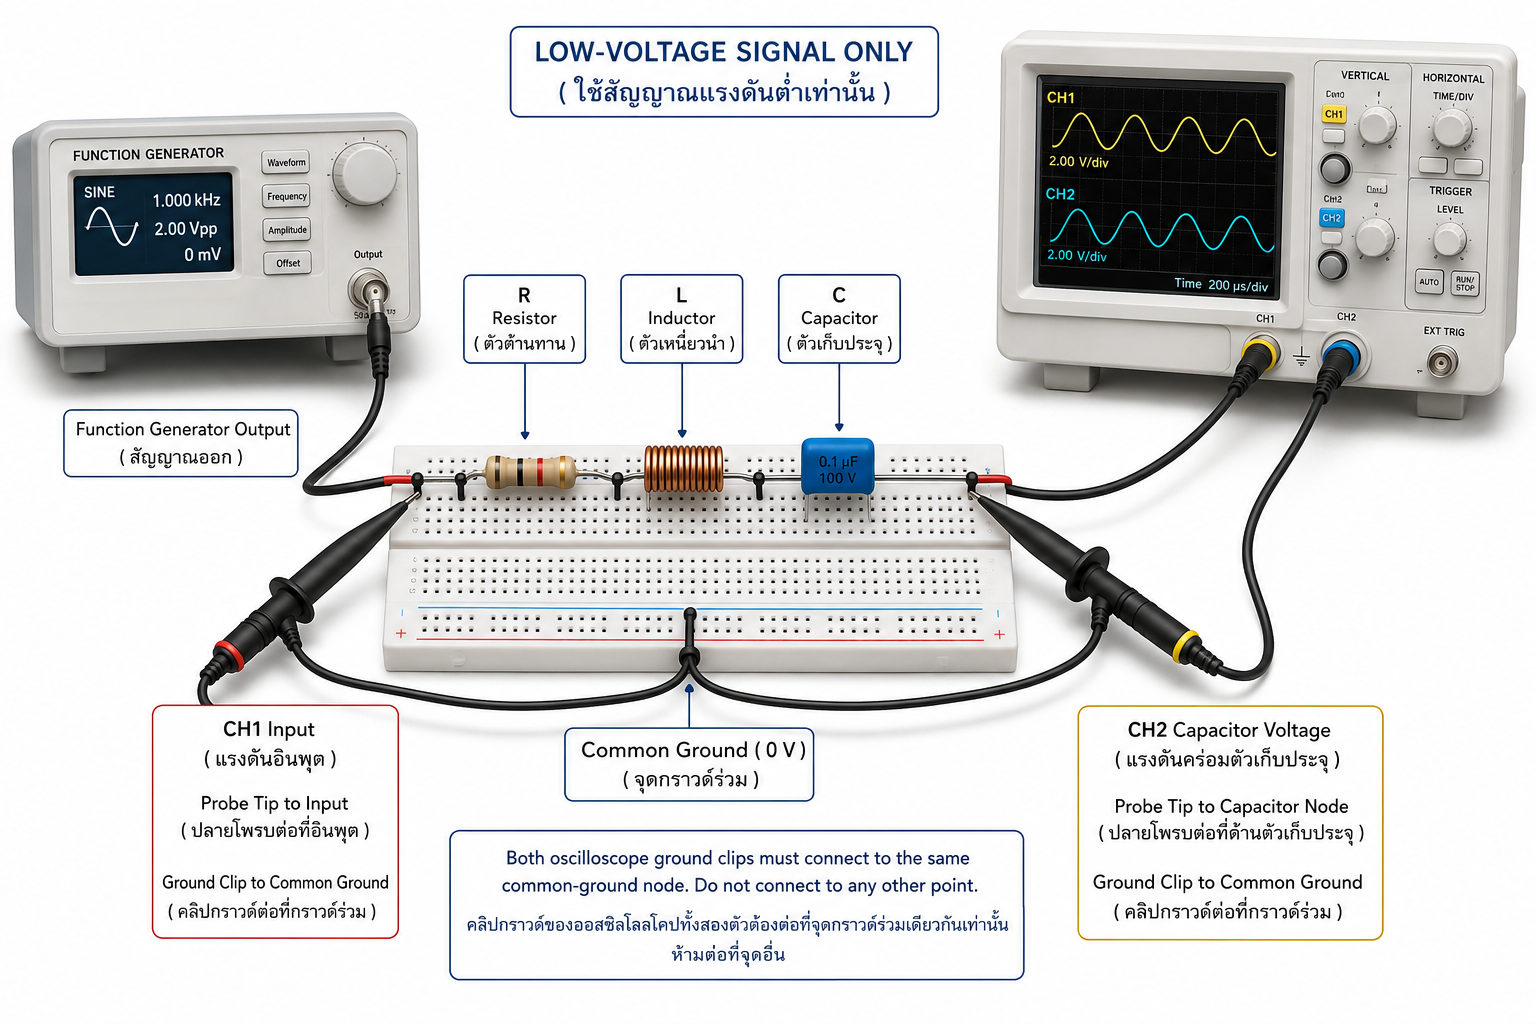
\includegraphics[width=0.8\textwidth]{images/chapter3/figure-10.png}
    \caption{ชุดทดลองวงจร RLC และจุดต่อ Oscilloscope}
\end{figure}

\subsubsection{9.4 ข้อควรระวังด้านความปลอดภัย}

\begin{enumerate}
    \item ใช้เฉพาะสัญญาณแรงดันต่ำจาก Function Generator ของห้องปฏิบัติการ \textbf{ห้ามต่อวงจรนี้เข้ากับไฟบ้านหรือแหล่งจ่ายที่ไม่แยกอย่างเหมาะสม}
    \item ปิดเอาต์พุต Function Generator ก่อนต่อหรือเปลี่ยนวงจร
    \item ตรวจสอบแผนผังรางของเบรดบอร์ดก่อนจ่ายสัญญาณ
    \item ตรวจสอบพิกัดกำลังของตัวต้านทานและพิกัดแรงดันของตัวเก็บประจุ
    \item Oscilloscope แบบตั้งโต๊ะทั่วไปมีกราวด์หัววัดเชื่อมกับสายดินป้องกัน จึงต้องต่อกราวด์ของทุกช่องที่โหนดกราวด์ร่วมเดียวกันเท่านั้น (Tektronix, n.d.)
    \item ห้ามคีบกราวด์หัววัดคร่อมองค์ประกอบหรือโหนดที่ไม่ใช่กราวด์ร่วม เพราะอาจทำให้โหนดนั้นถูกลัดวงจรลงดิน
    \item ห้ามเปลี่ยนการต่อวงจรขณะที่มีสัญญาณ
    \item หากอุปกรณ์ร้อน มีกลิ่นผิดปกติ หรือรูปคลื่นผิดปกติมาก ให้ปิดเอาต์พุตทันทีและแจ้งผู้สอน
    \item จัดสายให้เป็นระเบียบและหลีกเลี่ยงการสัมผัสตัวนำเปลือย
    \item การวัดวงจรที่ไม่อ้างอิงกราวด์หรือมีแรงดันสูงต้องใช้หัววัดและวิธีเฉพาะภายใต้การดูแลของผู้เชี่ยวชาญ ซึ่งไม่อยู่ในกิจกรรมนี้
\end{enumerate}

\subsubsection{9.5 ขั้นตอนการปฏิบัติ}

\paragraph{ตอนที่ 1: วัดพารามิเตอร์จริง}

\begin{enumerate}
    \item ปิด Function Generator และถอดแหล่งสัญญาณออกจากวงจร
    \item ใช้เครื่องมือวัดค่า $R$, $L$, $C$
    \item วัดความต้านทาน DC ของขดลวด $r_L$
    \item บันทึกค่าความต้านทานเอาต์พุตของ Function Generator จากคู่มือหรือค่าที่ผู้สอนกำหนด
    \item คำนวณ $R_{\text{eq}}$
\end{enumerate}

\paragraph{ตอนที่ 2: ต่อวงจร}

\begin{enumerate}
    \item ต่อ $R$, $L$, $C$ แบบอนุกรมบนเบรดบอร์ด
    \item กำหนดโหนดสุดท้ายของตัวเก็บประจุเป็นกราวด์ร่วม
    \item ต่อ Function Generator ที่อินพุตและกราวด์ร่วม
    \item ต่อ CH1 วัด $v_i(t)$ เทียบกราวด์ร่วม
    \item ต่อ CH2 วัด $v_o(t)=v_C(t)$ เทียบกราวด์ร่วม
    \item ให้ผู้สอนตรวจสอบก่อนเปิดสัญญาณ
\end{enumerate}

\paragraph{ตอนที่ 3: ตรวจสอบสัญญาณเบื้องต้น}

\begin{enumerate}
    \item ตั้งสัญญาณไซน์ประมาณ $1\ \text{V}_{pp}$, offset $0\ \text{V}$
    \item เริ่มที่ความถี่ต่ำกว่าความถี่ธรรมชาติอย่างน้อยหนึ่งลำดับขนาด เช่น $100\ \text{Hz}$
    \item ตรวจสอบว่า $v_o$ ใกล้ $v_i$ ที่ความถี่ต่ำ
    \item ตรวจสอบ Probe Ratio, Coupling และ Scale ของทั้งสองช่อง
    \item หากวงจรทำงานปกติ จึงเริ่มกวาดความถี่
\end{enumerate}

\paragraph{ตอนที่ 4: กวาดความถี่และบันทึกผล}

เลือกอย่างน้อย 10–15 จุดที่ครอบคลุมช่วงต่ำกว่า ใกล้ และสูงกว่าความถี่ธรรมชาติ ตัวอย่างช่วง $100$–$10{,}000\ \text{Hz}$ โดยเพิ่มจำนวนจุดใกล้บริเวณยอดเรโซแนนซ์

ในแต่ละความถี่

\begin{enumerate}
    \item รักษาแอมพลิจูดอินพุตให้คงที่
    \item วัด $V_{i,\text{pp}}$
    \item วัด $V_{o,\text{pp}}$
    \item วัด $\Delta t$ และระบุว่าเอาต์พุตนำหรือล้าหลัง
    \item คำนวณ $|G|$, $G_{\text{dB}}$ และ $\phi$
    \item บันทึกภาพหน้าจออย่างน้อยสามจุด: ความถี่ต่ำ ใกล้เรโซแนนซ์ และความถี่สูง
\end{enumerate}

\paragraph{ตอนที่ 5: สร้างแบบจำลองใน Simulink}

\begin{enumerate}
    \item สร้างแบบจำลอง \texttt{Transfer Fcn}
    \item แบบจำลองอุดมคติใช้ \texttt{[L*C R*C 1]}
    \item แบบจำลองเชิงปฏิบัติใช้ \texttt{[L*C Req*C 1]}
    \item ใช้ \texttt{Sine Wave} หรือสร้างการวิเคราะห์ความถี่ใน MATLAB ตามเครื่องมือที่มี
    \item จำลองที่ความถี่เดียวกับการทดลอง
    \item บันทึกแอมพลิจูดและเฟสของแบบจำลอง
    \item สร้างกราฟเปรียบเทียบข้อมูลทดลอง แบบจำลองอุดมคติ และแบบจำลองเชิงปฏิบัติ
\end{enumerate}

\subsubsection{9.6 ตารางบันทึกผล}

\paragraph{ตารางที่ 1 ค่าพารามิเตอร์}

\begin{table}[htbp]
    \centering
    \begin{tabular}{l r r l r}
        \hline
        \textbf{พารามิเตอร์} & \textbf{ค่าป้ายกำกับ} & \textbf{ค่าที่วัด} & \textbf{หน่วย} & \textbf{ความคลาดเคลื่อน (\%)} \\
        \hline
        $R$ &  &  & $\Omega$ &  \\
        $L$ &  &  & mH &  \\
        $r_L$ & ไม่ระบุ &  & $\Omega$ & — \\
        $C$ &  &  & $\mu$F &  \\
        $R_s$ &  &  & $\Omega$ &  \\
        $R_{\text{eq}}$ & — &  & $\Omega$ & — \\
        \hline
    \end{tabular}
\end{table}

\paragraph{ตารางที่ 2 ผลตอบสนองความถี่}

\begin{table}[htbp]
    \centering
    \begin{tabular}{r r r r r r r r l}
        \hline
        \textbf{ลำดับ} & \textbf{$f$ (Hz)} & \textbf{$V_{i,pp}$ (V)} & \textbf{$V_{o,pp}$ (V)} & \textbf{$|G|$} & \textbf{$G_{\text{dB}}$ (dB)} & \textbf{$\Delta t$ (s)} & \textbf{$\phi$ (deg)} & \textbf{หมายเหตุ} \\
        \hline
        1 &  &  &  &  &  &  &  &  \\
        2 &  &  &  &  &  &  &  &  \\
        3 &  &  &  &  &  &  &  &  \\
        4 &  &  &  &  &  &  &  &  \\
        5 &  &  &  &  &  &  &  &  \\
        6 &  &  &  &  &  &  &  &  \\
        7 &  &  &  &  &  &  &  &  \\
        8 &  &  &  &  &  &  &  &  \\
        9 &  &  &  &  &  &  &  &  \\
        10 &  &  &  &  &  &  &  &  \\
        11 &  &  &  &  &  &  &  &  \\
        12 &  &  &  &  &  &  &  &  \\
        \hline
    \end{tabular}
\end{table}

\paragraph{ตารางที่ 3 การเปรียบเทียบแบบจำลอง}

\begin{table}[htbp]
    \centering
    \begin{tabular}{r r r r r r}
        \hline
        \textbf{$f$ (Hz)} & \textbf{$|G|_{\text{meas}}$} & \textbf{$|G|_{\text{ideal}}$} & \textbf{$|G|_{\text{practical}}$} & \textbf{Error ideal (\%)} & \textbf{Error practical (\%)} \\
        \hline
         &  &  &  &  &  \\
         &  &  &  &  &  \\
         &  &  &  &  &  \\
        \hline
    \end{tabular}
\end{table}

\subsubsection{9.7 การคำนวณและวิเคราะห์ผล}

\begin{enumerate}
    \item ใช้ค่าที่วัดจริงสร้าง $G_{\text{ideal}}(s)$
    \item รวม $R_s$ และ $r_L$ เพื่อสร้าง $G_{\text{practical}}(s)$
    \item คำนวณ $\omega_n$, $f_n$ และ $\zeta$ ของทั้งสองแบบจำลอง
    \item คำนวณขนาดและเฟสตามความถี่ที่ทดลอง
    \item สร้างกราฟแกนความถี่ลอการิทึม
    \item เปรียบเทียบตำแหน่งและขนาดยอดเรโซแนนซ์
    \item คำนวณความคลาดเคลื่อนแบบจุดต่อจุด
    \item อภิปรายว่าพารามิเตอร์ใดมีผลต่อความแตกต่างมากที่สุด
\end{enumerate}

ตัวอย่างความคลาดเคลื่อนขนาดอัตราขยาย

\[
\%\text{Error}_k
=
\left|
\frac{|G|_{\text{meas},k}-|G|_{\text{model},k}}
{|G|_{\text{model},k}}
\right|\times100
\]

เมื่อค่าตัวหารใกล้ศูนย์ ควรหลีกเลี่ยงการตีความเปอร์เซ็นต์เพียงอย่างเดียวและรายงานความคลาดเคลื่อนสัมบูรณ์ร่วมด้วย

\subsubsection{9.8 การเปรียบเทียบผลจริงกับทฤษฎีหรือแบบจำลอง}

รายงานควรประกอบด้วย

\begin{itemize}
    \item ตารางพารามิเตอร์จริง
    \item Transfer Function อุดมคติและเชิงปฏิบัติ
    \item กราฟขนาดและเฟสสามชุด
    \item ภาพหน้าจอ Oscilloscope
    \item ค่าเรโซแนนซ์จากทฤษฎี จำลอง และทดลอง
    \item การอภิปรายโหลดจากเครื่องมือวัด
    \item การอภิปรายค่าคลาดเคลื่อนของอุปกรณ์
    \item ข้อเสนอปรับปรุงแบบจำลองหรือวิธีทดลอง
\end{itemize}

\textbf{ห้ามสร้างหรือเติมค่าที่ไม่ได้วัดจริง} หากข้อมูลบางจุดใช้ไม่ได้ ให้ระบุสาเหตุและทำซ้ำการวัด

\subsubsection{9.9 คำถามหลังการทดลอง}

\begin{enumerate}
    \item เหตุใด $R_{\text{eq}}$ จึงทำให้ยอดเรโซแนนซ์ลดลง
    \item หากเพิ่ม $R$ เป็นสองเท่า ค่า $\omega_n$ และ $\zeta$ เปลี่ยนอย่างไร
    \item เหตุใดแรงดันคร่อมตัวเก็บประจุอาจสูงกว่าแรงดันอินพุตใกล้เรโซแนนซ์
    \item ความต้านทานอินพุตและความจุของหัววัดมีผลต่อวงจรอย่างไร
    \item หากวัดเอาต์พุตคร่อมตัวต้านทาน ฟังก์ชันถ่ายโอนจะเปลี่ยนเป็นแบบใด
    \item เพราะเหตุใดกราฟเฟสจากการวัด $\Delta t$ จึงอ่านยากเมื่อความถี่สูง
    \item แบบจำลองอุดมคติหรือเชิงปฏิบัติสอดคล้องกับผลทดลองมากกว่า เพราะเหตุใด
    \item หากผลจำลองไม่ตรงสมการคำนวณ ควรตรวจสอบรายการใดก่อน
\end{enumerate}

\subsubsection{9.10 เกณฑ์การประเมินกิจกรรมปฏิบัติการ}

\begin{table}[htbp]
    \centering
    \begin{tabular}{l r l l l}
        \hline
        \textbf{ด้านประเมิน} & \textbf{น้ำหนัก} & \textbf{ดีเยี่ยม} & \textbf{ผ่านเกณฑ์} & \textbf{ต้องปรับปรุง} \\
        \hline
        ความถูกต้องของการต่อวงจร & 15\% & ต่อถูกและตรวจสอบเป็นระบบ & มีข้อผิดพลาดเล็กน้อย แก้ไขได้ & ต่อผิดหรือไม่ตรวจสอบ \\
        ความปลอดภัยและการใช้เครื่องมือ & 15\% & ปฏิบัติตามข้อกำหนดครบ & มีการเตือนเล็กน้อย & เสี่ยงต่ออุปกรณ์หรือผู้ใช้ \\
        การวัดและบันทึกข้อมูล & 20\% & ข้อมูลครบ หน่วยและเงื่อนไขชัด & ขาดบางจุดแต่ยังวิเคราะห์ได้ & ข้อมูลไม่พอหรือไม่น่าเชื่อถือ \\
        การคำนวณ Transfer Function & 15\% & สมการและพารามิเตอร์ถูกต้อง & ผิดเล็กน้อย & ไม่สามารถเชื่อมสมการกับวงจร \\
        แบบจำลอง MATLAB/Simulink & 15\% & สร้างและตรวจสอบได้ครบ & แบบจำลองทำงานแต่ขาดการตรวจสอบ & แบบจำลองไม่ทำงาน \\
        การเปรียบเทียบและอภิปราย & 15\% & อธิบายความคลาดเคลื่อนด้วยเหตุผล & เปรียบเทียบได้ระดับพื้นฐาน & สรุปโดยไม่มีหลักฐาน \\
        รายงานและการสื่อสาร & 5\% & ชัดเจน เป็นระบบ อ้างรูปและตาราง & อ่านเข้าใจได้ & ไม่เป็นระบบ \\
        \hline
    \end{tabular}
\end{table}

\par\noindent\rule{\textwidth}{0.4pt}\par

\subsection{10. ความเข้าใจผิดที่พบบ่อย}

\begin{table}[htbp]
    \centering
    \begin{tabular}{l l}
        \hline
        \textbf{ความเข้าใจคลาดเคลื่อน} & \textbf{แนวคิดที่ถูกต้อง} \\
        \hline
        ฟังก์ชันถ่ายโอนคืออัตราส่วน $y(t)/u(t)$ & ต้องเป็นอัตราส่วน $Y(s)/U(s)$ ในโดเมนลาปลาซ ภายใต้เงื่อนไขที่กำหนด \\
        ค่าเริ่มต้นไม่เกี่ยวกับ Transfer Function & การนิยามแบบมาตรฐานใช้อัตราส่วนภายใต้ค่าเริ่มต้นเป็นศูนย์ \\
        วงจรหรือระบบหนึ่งมี Transfer Function เพียงชุดเดียว & ฟังก์ชันถ่ายโอนขึ้นกับการเลือกอินพุตและเอาต์พุต \\
        จำนวนองค์ประกอบสะสมพลังงานเท่ากับอันดับเสมอ & อาจมีข้อจำกัดหรือการพึ่งพากัน ทำให้อันดับลดลง \\
        ใช้ตัวหารแรงดันกับอิมพีแดนซ์ได้โดยไม่สนใจค่าเริ่มต้น & รูปอิมพีแดนซ์ $sL$ และ $1/(sC)$ แบบง่ายสอดคล้องกับค่าเริ่มต้นเป็นศูนย์ \\
        โพลคือค่าพารามิเตอร์ทางกายภาพโดยตรง & โพลเป็นรากของสมการลักษณะเฉพาะและเกิดจากการรวมพารามิเตอร์ \\
        State-Space ที่แปลงจาก Transfer Function มีเพียงรูปเดียว & realization ไม่เป็นเอกลักษณ์ แม้ให้พฤติกรรมอินพุต–เอาต์พุตเดียวกัน \\
        ผล Simulink คือความจริงของระบบ & ผลจำลองถูกต้องตามแบบจำลองและค่าพารามิเตอร์ที่ใส่เท่านั้น \\
        กราวด์หัววัด Oscilloscope ต่อที่ใดก็ได้ & สำหรับเครื่องตั้งโต๊ะทั่วไป กราวด์หัววัดมักผูกกับสายดิน ต้องต่อที่โหนดกราวด์ร่วม \\
        เพิ่มรายละเอียดมากทำให้แบบจำลองดีกว่าเสมอ & แบบจำลองควรละเอียดพอสำหรับวัตถุประสงค์ แต่ไม่ซับซ้อนเกินจำเป็น \\
        \hline
    \end{tabular}
\end{table}

\par\noindent\rule{\textwidth}{0.4pt}\par

\subsection{11. การประยุกต์ใช้ในงานจริง}

\subsubsection{11.1 ระบบกันสะเทือนและเครื่องจักร}

แบบจำลองมวล–สปริง–ตัวหน่วงใช้ประมาณการสั่นสะเทือนของยานพาหนะ เครื่องจักร โครงสร้าง และระบบแยกแรงสั่น การวิเคราะห์ช่วยเลือกความแข็งและการหน่วงเพื่อหลีกเลี่ยงเรโซแนนซ์หรือจำกัดการสั่น

\subsubsection{11.2 วงจรกรองและระบบวัด}

RC, RL และ RLC ใช้เป็นพื้นฐานของวงจรกรอง สัญญาณปรับสภาพ และอินเทอร์เฟซเซนเซอร์ Transfer Function ช่วยประเมินแบนด์วิดท์ การลดทอน และเฟสก่อนสร้างวงจรจริง

\subsubsection{11.3 ระบบขับเคลื่อนด้วยมอเตอร์}

แบบจำลองมอเตอร์ DC เชื่อมแรงดัน กระแส แรงบิด และความเร็ว ใช้เลือกตัวควบคุมความเร็ว ตำแหน่ง หรือแรงบิด และใช้ประเมินผลกระทบจากโหลดรบกวน

\subsubsection{11.4 ระบบควบคุมกระบวนการ}

แม้กระบวนการจริงอาจซับซ้อน แต่แบบจำลองอันดับหนึ่งหรืออันดับสองสามารถใช้ประมาณพฤติกรรมรอบจุดทำงาน เช่น อุณหภูมิ ระดับของเหลว และอัตราการไหล เพื่อออกแบบตัวควบคุมเบื้องต้น

\subsubsection{11.5 Digital Twin และ Model-Based Design}

แนวคิดการสร้างแบบจำลองเป็นฐานของการออกแบบโดยใช้แบบจำลอง การทดสอบแบบจำลองก่อนฮาร์ดแวร์ และ Digital Twin อย่างไรก็ตาม แบบจำลองต้องผ่านการปรับพารามิเตอร์และตรวจสอบกับข้อมูลจริงอย่างต่อเนื่อง

\par\noindent\rule{\textwidth}{0.4pt}\par

\subsection{12. สรุปท้ายบท}

\begin{enumerate}
    \item แบบจำลองทางคณิตศาสตร์เป็นตัวแทนของพฤติกรรมระบบภายใต้สมมติฐานและขอบเขตที่ชัดเจน
    \item กระบวนการสำคัญคือกำหนดระบบ เลือกอินพุต–เอาต์พุต ใช้กฎทางฟิสิกส์ สร้างสมการเชิงอนุพันธ์ แปลงลาปลาซ และตรวจสอบแบบจำลอง
    \item ฟังก์ชันถ่ายโอนของระบบ LTI นิยามเป็น
\end{enumerate}

\[
G(s)=\frac{Y(s)}{U(s)}
\]

ภายใต้ค่าเริ่มต้นเป็นศูนย์

\begin{enumerate}
    \item โพล ซีโร และอัตราขยายให้ข้อมูลเชิงโครงสร้างของพฤติกรรมอินพุต–เอาต์พุต
    \item ระบบมวล–สปริง–ตัวหน่วงมี
\end{enumerate}

\[
\frac{X(s)}{F(s)}=\frac{1}{ms^2+cs+k}
\]

\begin{enumerate}
    \item วงจร RC ผ่านต่ำมี
\end{enumerate}

\[
\frac{V_C(s)}{V_i(s)}=\frac{1}{RCs+1}
\]

\begin{enumerate}
    \item วงจร RLC อนุกรมที่วัดคร่อม $C$ มี
\end{enumerate}

\[
\frac{V_C(s)}{V_i(s)}=\frac{1}{LCs^2+RCs+1}
\]

\begin{enumerate}
    \item มอเตอร์ DC ต้องเชื่อมสมการวงจรอาร์เมเจอร์กับสมการกล และมี Back EMF เป็นป้อนกลับภายใน
    \item State-Space แสดงพลวัตภายใน และ realization ของ Transfer Function ไม่เป็นเอกลักษณ์
    \item MATLAB/Simulink เป็นเครื่องมือช่วยคำนวณและจำลอง แต่ไม่แทนการตรวจสอบสมมติฐาน หน่วย และผลทดลอง
    \item ความต่างระหว่างผลทดลองกับแบบจำลองสามารถใช้ระบุพารามิเตอร์แฝงและปรับปรุงแบบจำลองให้เหมาะกับวัตถุประสงค์
\end{enumerate}

\par\noindent\rule{\textwidth}{0.4pt}\par

\subsection{13. คำถามทบทวน}

\begin{enumerate}
    \item แบบจำลองทางคณิตศาสตร์มีบทบาทอย่างไรในการออกแบบระบบควบคุม
    \item อธิบายเงื่อนไขสำคัญของการนิยาม Transfer Function
    \item เพราะเหตุใดต้องกำหนดอินพุตและเอาต์พุตก่อนสร้างแบบจำลอง
    \item อธิบายความหมายของโพล ซีโร และอัตราขยาย
    \item เปรียบเทียบระบบอันดับหนึ่งกับระบบอันดับสอง
    \item เขียนขั้นตอนการสร้างแบบจำลองมวล–สปริง–ตัวหน่วง
    \item วงจร RL เดียวกันให้พฤติกรรมผ่านต่ำหรือผ่านสูงได้อย่างไร
    \item Back EMF ของมอเตอร์ DC มีผลต่อความเร็วอย่างไร
    \item Transfer Function และ State-Space ต่างกันในด้านข้อมูลที่แสดงอย่างไร
    \item ระบุสาเหตุอย่างน้อยสี่ประการที่ทำให้ผลทดลองต่างจากผลจำลอง
\end{enumerate}

\par\noindent\rule{\textwidth}{0.4pt}\par

\subsection{14. แบบฝึกหัดท้ายบท}

\subsubsection{14.1 ระดับพื้นฐาน}

\textbf{ข้อ 1} อธิบายความหมายของแบบจำลองทางคณิตศาสตร์ และยกตัวอย่างสมมติฐานหนึ่งข้อที่ใช้ในการสร้างแบบจำลองระบบจริง

\textbf{ข้อ 2} กำหนดสมการ

\[
3\dot{y}(t)+6y(t)=2u(t)
\]

จงหา $G(s)=Y(s)/U(s)$ ภายใต้ค่าเริ่มต้นเป็นศูนย์ พร้อมระบุอันดับ โพล และอัตราขยาย DC

\textbf{ข้อ 3} วงจร RC ผ่านต่ำมี $R=10\ \text{k}\Omega$ และ $C=10\ \mu\text{F}$ จงหาค่าคงตัวเวลาและความถี่ตัด

\textbf{ข้อ 4} จงอธิบายเหตุผลที่ Transfer Function มาตรฐานต้องกำหนดค่าเริ่มต้นเป็นศูนย์

\textbf{ข้อ 5} ให้

\[
G(s)=\frac{5}{s^2+4s+5}
\]

จงระบุเมทริกซ์ $A,B,C,D$ ในรูป controllable canonical form หนึ่งรูป

\subsubsection{14.2 ระดับวิเคราะห์}

\textbf{ข้อ 6} ระบบมวล–สปริง–ตัวหน่วงมี $m=4\ \text{kg}$, $c=8\ \text{N·s/m}$ และ $k=16\ \text{N/m}$ อินพุตเป็นแรง เอาต์พุตเป็นการกระจัด จงสร้างสมการเชิงอนุพันธ์ หา Transfer Function, $\omega_n$ และ $\zeta$

\textbf{ข้อ 7} วงจร RL อนุกรมมี $R=20\ \Omega$ และ $L=0.2\ \text{H}$\\ก. หา Transfer Function เมื่อวัดเอาต์พุตคร่อม $R$\\ข. หา Transfer Function เมื่อวัดเอาต์พุตคร่อม $L$\\ค. อธิบายพฤติกรรมที่ความถี่ต่ำและสูง

\textbf{ข้อ 8} วงจร RLC อนุกรมมี $R=50\ \Omega$, $L=20\ \text{mH}$, $C=5\ \mu\text{F}$ วัดเอาต์พุตคร่อม $C$ จงหา Transfer Function, $\omega_n$, $f_n$ และ $\zeta$

\textbf{ข้อ 9} วงจร Op-Amp กลับเฟสมี $R_{in}=10\ \text{k}\Omega$, $R_f=100\ \text{k}\Omega$ และ $C_f=10\ \text{nF}$ ต่อ $C_f$ ขนานกับ $R_f$ จงหา Transfer Function อัตราขยายความถี่ต่ำ และความถี่โพล

\textbf{ข้อ 10} มอเตอร์ DC มี

\[
J=0.02,\quad b=0.05,\quad
R_a=2,\quad L_a=0.1,\quad
K_t=K_e=0.2
\]

ใช้หน่วย SI จงหา $\Omega(s)/V_a(s)$ เมื่อ $T_L=0$ และหาอัตราขยาย DC

\subsubsection{14.3 ระดับประยุกต์ใช้}

\textbf{ข้อ 11} ในการทดลอง RLC ใช้ $R=100\ \Omega$, $L=10\ \text{mH}$, $C=1\ \mu\text{F}$ แต่ Function Generator มี $R_s=50\ \Omega$ และตัวเหนี่ยวนำมี $r_L=20\ \Omega$\\ก. สร้างแบบจำลองเชิงปฏิบัติ\\ข. เปรียบเทียบ $\zeta$ กับแบบจำลองอุดมคติ\\ค. อธิบายผลต่อยอดเรโซแนนซ์

\textbf{ข้อ 12} นักศึกษาสร้างแบบจำลอง Simulink ของวงจร RLC โดยใส่ Denominator เป็น \texttt{[1 R*C L*C]} และได้กราฟไม่ตรงกับการคำนวณ จงวิเคราะห์ข้อผิดพลาด เขียนเวกเตอร์ที่ถูกต้อง และเสนอรายการตรวจสอบอีกอย่างน้อยสามข้อ

\textbf{ข้อ 13} ผลทดลองของวงจร RLC มีความถี่ยอดอัตราขยายต่ำกว่าแบบจำลองอุดมคติ และยอดต่ำกว่าอย่างชัดเจน จงเสนอสมมติฐานสาเหตุอย่างน้อยสี่ข้อ ระบุวิธีตรวจสอบแต่ละข้อ และอธิบายว่าจะปรับแบบจำลองอย่างไร

\newpage

\subsection{15. แนวคำตอบและเฉลยแบบฝึกหัด}

\begin{quote}
\textbf{ส่วนสำหรับผู้สอน:} ควรแยกส่วนนี้ออกจากเอกสารนักศึกษาเมื่อใช้เป็นงานมอบหมายหรือการประเมิน
\end{quote}

\subsubsection{15.1 เฉลยระดับพื้นฐาน}

\paragraph{เฉลยข้อ 1}

\textbf{แนวคิดที่ใช้:} แบบจำลองทางคณิตศาสตร์เป็นการแทนความสัมพันธ์ของตัวแปรและพลวัตของระบบจริงด้วยสมการ เพื่อใช้วิเคราะห์ ทำนาย จำลอง หรือออกแบบระบบควบคุม

ตัวอย่างสมมติฐาน ได้แก่

\begin{itemize}
    \item สปริงทำงานในช่วงเชิงเส้น จึงใช้ $F_s=kx$
    \item แรงเสียดทานเป็นแบบหนืด จึงใช้ $F_d=c\dot{x}$
    \item ค่า $R$, $L$, $C$ คงที่
    \item Op-Amp ทำงานในช่วงไม่อิ่มตัว
    \item มอเตอร์ทำงานรอบจุดที่ค่าคงตัวแรงบิดและ Back EMF คงที่
\end{itemize}

\textbf{การแปลความหมาย:} แบบจำลองไม่ใช่สำเนาของระบบจริง แต่เป็นตัวแทนที่มีความละเอียดเหมาะกับวัตถุประสงค์ สมมติฐานจึงต้องระบุและตรวจสอบ

\paragraph{เฉลยข้อ 2}

กำหนด

\[
3\dot{y}(t)+6y(t)=2u(t)
\]

แปลงลาปลาซเมื่อ $y(0)=0$

\[
3sY(s)+6Y(s)=2U(s)
\]

จัดรูป

\[
(3s+6)Y(s)=2U(s)
\]

ดังนั้น

\[
\boxed{
G(s)=\frac{Y(s)}{U(s)}
=\frac{2}{3s+6}
=\frac{2/3}{s+2}
}
\]

\begin{itemize}
    \item อันดับระบบ: 1
    \item โพล: $s=-2$
    \item ซีโรจำกัด: ไม่มี
    \item อัตราขยาย DC:
\end{itemize}

\[
G(0)=\frac{2}{6}=\boxed{\frac{1}{3}}
\]

\textbf{ข้อผิดพลาดที่พบบ่อย:} ลืมว่าตัวคูณ 3 ต้องคงอยู่ทั้งก่อนและหลังแปลงลาปลาซ

\paragraph{เฉลยข้อ 3}

\[
R=10\ \text{k}\Omega=10{,}000\ \Omega
\]

\[
C=10\ \mu\text{F}=10\times10^{-6}\ \text{F}
\]

ค่าคงตัวเวลา

\[
\tau=RC
=(10{,}000)(10\times10^{-6})
=\boxed{0.1\ \text{s}}
\]

ความถี่ตัดเชิงมุม

\[
\omega_c=\frac{1}{RC}=10\ \text{rad/s}
\]

ความถี่ตัดหน่วยเฮิรตซ์

\[
f_c=\frac{1}{2\pi RC}
=\frac{1}{2\pi(0.1)}
\approx\boxed{1.59\ \text{Hz}}
\]

\paragraph{เฉลยข้อ 4}

เมื่อแปลงอนุพันธ์ด้วยลาปลาซ จะเกิดพจน์ค่าเริ่มต้น เช่น

\[
\mathcal{L}\{\dot{y}\}=sY(s)-y(0)
\]

หาก $y(0)\neq0$ ความสัมพันธ์ $Y(s)$ จะมีทั้งผลจากอินพุตและผลจากพลังงานเริ่มต้น จึงไม่สามารถนิยาม $Y(s)/U(s)$ เป็นคุณสมบัติของระบบเพียงอย่างเดียวได้อย่างตรงไปตรงมา การกำหนดค่าเริ่มต้นเป็นศูนย์ทำให้

\[
Y(s)=G(s)U(s)
\]

และ $G(s)$ ขึ้นกับพารามิเตอร์ระบบ ไม่ขึ้นกับอินพุตเฉพาะครั้งหรือสถานะเริ่มต้น

\paragraph{เฉลยข้อ 5}

ให้

\[
G(s)=\frac{5}{s^2+4s+5}
\]

เปรียบเทียบกับ

\[
G(s)=\frac{b_1s+b_0}{s^2+a_1s+a_0}
\]

ได้

\[
a_1=4,\quad a_0=5,\quad b_1=0,\quad b_0=5
\]

รูป controllable canonical form หนึ่งรูปคือ

\[
\boxed{
A=
\begin{bmatrix}
0 & 1\\
-5 & -4
\end{bmatrix},
\quad
B=
\begin{bmatrix}
0\\
1
\end{bmatrix},
\quad
C=
\begin{bmatrix}
5 & 0
\end{bmatrix},
\quad
D=0
}
\]

ตรวจสอบด้วย $G(s)=C(sI-A)^{-1}B+D$ จะได้ฟังก์ชันถ่ายโอนเดิม

\subsubsection{15.2 เฉลยระดับวิเคราะห์}

\paragraph{เฉลยข้อ 6}

กำหนด

\[
m=4\ \text{kg},\quad
c=8\ \text{N·s/m},\quad
k=16\ \text{N/m}
\]

สมการแรง

\[
F(t)-c\dot{x}(t)-kx(t)=m\ddot{x}(t)
\]

จัดรูป

\[
\boxed{
4\ddot{x}(t)+8\dot{x}(t)+16x(t)=F(t)
}
\]

แปลงลาปลาซภายใต้ค่าเริ่มต้นเป็นศูนย์

\[
(4s^2+8s+16)X(s)=F(s)
\]

ดังนั้น

\[
\boxed{
\frac{X(s)}{F(s)}
=
\frac{1}{4s^2+8s+16}
}
\]

ความถี่ธรรมชาติ

\[
\omega_n=\sqrt{\frac{k}{m}}
=\sqrt{\frac{16}{4}}
=\boxed{2\ \text{rad/s}}
\]

อัตราส่วนการหน่วง

\[
\zeta=\frac{c}{2\sqrt{mk}}
=
\frac{8}{2\sqrt{(4)(16)}}
=
\frac{8}{16}
=\boxed{0.5}
\]

ระบบเป็น underdamped เพราะ $0<\zeta<1$

\paragraph{เฉลยข้อ 7}

กำหนด $R=20\ \Omega$, $L=0.2\ \text{H}$

\textbf{ก. เอาต์พุตคร่อม ZZPROTECTED0ZZ}

\[
\frac{V_R(s)}{V_i(s)}
=
\frac{R}{Ls+R}
=
\frac{20}{0.2s+20}
\]

หารด้วย $0.2$

\[
\boxed{
G_R(s)=\frac{100}{s+100}
}
\]

\textbf{ข. เอาต์พุตคร่อม ZZPROTECTED0ZZ}

\[
\frac{V_L(s)}{V_i(s)}
=
\frac{Ls}{Ls+R}
=
\frac{0.2s}{0.2s+20}
\]

\[
\boxed{
G_L(s)=\frac{s}{s+100}
}
\]

\textbf{ค. พฤติกรรม}

\begin{itemize}
    \item เมื่อ $\omega\rightarrow0$: $G_R(j\omega)\rightarrow1$, $G_L(j\omega)\rightarrow0$
    \item เมื่อ $\omega\rightarrow\infty$: $G_R(j\omega)\rightarrow0$, $G_L(j\omega)\rightarrow1$
\end{itemize}

ดังนั้นเอาต์พุตคร่อม $R$ เป็นผ่านต่ำ และเอาต์พุตคร่อม $L$ เป็นผ่านสูง

\paragraph{เฉลยข้อ 8}

กำหนด

\[
R=50\ \Omega,\quad
L=20\ \text{mH}=0.02\ \text{H}
\]

\[
C=5\ \mu\text{F}=5\times10^{-6}\ \text{F}
\]

คำนวณ

\[
LC=(0.02)(5\times10^{-6})=1\times10^{-7}
\]

\[
RC=(50)(5\times10^{-6})=2.5\times10^{-4}
\]

Transfer Function

\[
\boxed{
G(s)=
\frac{1}{10^{-7}s^2+2.5\times10^{-4}s+1}
}
\]

หรือ

\[
\boxed{
G(s)=
\frac{10^7}{s^2+2500s+10^7}
}
\]

ความถี่ธรรมชาติ

\[
\omega_n=\frac{1}{\sqrt{LC}}
=\frac{1}{\sqrt{10^{-7}}}
\approx\boxed{3162.28\ \text{rad/s}}
\]

\[
f_n=\frac{\omega_n}{2\pi}
\approx\boxed{503.29\ \text{Hz}}
\]

อัตราส่วนการหน่วง

\[
\zeta=
\frac{R}{2}\sqrt{\frac{C}{L}}
=
25\sqrt{\frac{5\times10^{-6}}{0.02}}
\]

\[
\zeta
=25\sqrt{2.5\times10^{-4}}
\approx\boxed{0.395}
\]

ระบบเป็น underdamped และมีแนวโน้มเกิดยอดเรโซแนนซ์

\paragraph{เฉลยข้อ 9}

กำหนด

\[
R_{in}=10\ \text{k}\Omega,\quad
R_f=100\ \text{k}\Omega,\quad
C_f=10\ \text{nF}
\]

Transfer Function

\[
G(s)=
-\frac{R_f/R_{in}}{1+sR_fC_f}
\]

อัตราขยายความถี่ต่ำ

\[
-\frac{R_f}{R_{in}}
=-\frac{100}{10}
=\boxed{-10}
\]

ค่าคงตัวเวลา

\[
R_fC_f=(100\times10^3)(10\times10^{-9})
=10^{-3}\ \text{s}
\]

ดังนั้น

\[
\boxed{
G(s)=\frac{-10}{1+0.001s}
}
\]

ความถี่โพล

\[
\omega_p=\frac{1}{R_fC_f}
=\boxed{1000\ \text{rad/s}}
\]

\[
f_p=\frac{1000}{2\pi}
\approx\boxed{159.15\ \text{Hz}}
\]

\paragraph{เฉลยข้อ 10}

สมการทั่วไป

\[
\frac{\Omega(s)}{V_a(s)}
=
\frac{K_t}
{L_aJs^2+(L_ab+R_aJ)s+(R_ab+K_tK_e)}
\]

แทนค่า

\[
L_aJ=(0.1)(0.02)=0.002
\]

\[
L_ab+R_aJ=(0.1)(0.05)+(2)(0.02)
=0.005+0.04=0.045
\]

\[
R_ab+K_tK_e=(2)(0.05)+(0.2)(0.2)
=0.1+0.04=0.14
\]

จึงได้

\[
\boxed{
\frac{\Omega(s)}{V_a(s)}
=
\frac{0.2}{0.002s^2+0.045s+0.14}
}
\]

หารทั้งเศษและส่วนด้วย $0.002$

\[
\boxed{
\frac{\Omega(s)}{V_a(s)}
=
\frac{100}{s^2+22.5s+70}
}
\]

อัตราขยาย DC

\[
G(0)=\frac{0.2}{0.14}
\approx\boxed{1.429\ \frac{\text{rad/s}}{\text{V}}}
\]

\subsubsection{15.3 เฉลยระดับประยุกต์ใช้}

\paragraph{เฉลยข้อ 11}

กำหนด

\[
R=100\ \Omega,\quad
R_s=50\ \Omega,\quad
r_L=20\ \Omega
\]

ดังนั้น

\[
R_{\text{eq}}=100+50+20=170\ \Omega
\]

\textbf{ก. แบบจำลองเชิงปฏิบัติ}

เมื่อ $L=10^{-2}\ \text{H}$ และ $C=10^{-6}\ \text{F}$

\[
LC=10^{-8}
\]

\[
R_{\text{eq}}C=(170)(10^{-6})=1.7\times10^{-4}
\]

จึงได้

\[
\boxed{
G_p(s)
=
\frac{1}{10^{-8}s^2+1.7\times10^{-4}s+1}
}
\]

\textbf{ข. เปรียบเทียบอัตราส่วนการหน่วง}

แบบอุดมคติที่ใช้ $R=100\ \Omega$

\[
\zeta_{\text{ideal}}
=
\frac{100}{2}\sqrt{\frac{10^{-6}}{10^{-2}}}
=0.5
\]

แบบเชิงปฏิบัติ

\[
\zeta_{\text{practical}}
=
\frac{170}{2}\sqrt{\frac{10^{-6}}{10^{-2}}}
=85(0.01)
=\boxed{0.85}
\]

\textbf{ค. ผลต่อยอดเรโซแนนซ์}

การเพิ่มความต้านทานทำให้การหน่วงสูงขึ้น จาก $\zeta=0.5$ เป็น $0.85$ สำหรับรูปผ่านต่ำอันดับสอง เมื่อ $\zeta\geq1/\sqrt{2}$ จะไม่มียอดเรโซแนนซ์ของขนาดอัตราขยายแบบเด่นชัด ดังนั้นผลจริงควรมียอดต่ำกว่าหรือไม่มีจุดยอดชัดเมื่อเทียบกับแบบอุดมคติ

\paragraph{เฉลยข้อ 12}

สมการส่วนของวงจรคือ

\[
LCs^2+RCs+1
\]

เวกเตอร์สัมประสิทธิ์ต้องเรียงจากกำลังสูงไปต่ำ คือ

\[
\boxed{[L*C,\ R*C,\ 1]}
\]

สำหรับค่าตัวอย่าง $L=10\ \text{mH}$, $C=1\ \mu\text{F}$, $R=100\ \Omega$

\[
\boxed{[1e-8,\ 1e-4,\ 1]}
\]

การใส่ \texttt{[1 R*C L*C]} แทนพหุนาม

\[
s^2+RCs+LC
\]

ซึ่งไม่ใช่สมการเดิมและมีหน่วยไม่สอดคล้องกัน

รายการตรวจสอบเพิ่มเติม

\begin{enumerate}
    \item แปลง mH และ $\mu$F เป็น H และ F แล้วหรือไม่
    \item Numerator ถูกต้องหรือไม่
    \item Stop Time ยาวพอหรือไม่
    \item Solver และ Max Step Size เหมาะกับไดนามิกเร็วหรือไม่
    \item ค่าเริ่มต้นของ Integrator ตรงกันหรือไม่
    \item เลือกเอาต์พุตคร่อมองค์ประกอบเดียวกับแบบจำลองหรือไม่
    \item สัญญาณป้อนเข้ามีแอมพลิจูดและหน่วยตรงกันหรือไม่
\end{enumerate}

\paragraph{เฉลยข้อ 13}

ตัวอย่างการวิเคราะห์อย่างเป็นระบบ

\begin{table}[htbp]
    \centering
    \begin{tabular}{l l l}
        \hline
        \textbf{สมมติฐานสาเหตุ} & \textbf{วิธีตรวจสอบ} & \textbf{การปรับแบบจำลอง} \\
        \hline
        มี $R_s$ และ $r_L$ ที่ละเลย & อ่านสเปก Function Generator และวัดความต้านทานขดลวด & ใช้ $R_{\text{eq}}=R+R_s+r_L$ \\
        ค่า $L$ หรือ $C$ จริงต่างจากป้าย & วัดด้วย LCR Meter & แทนค่าที่วัดจริง \\
        ตัวเก็บประจุมี ESR & ใช้เครื่องมือวัด ESR หรือเปรียบเทียบหลายชนิด & เพิ่ม $R_{\text{ESR}}$ ในแบบจำลอง \\
        หัววัดและ Oscilloscope โหลดวงจร & ตรวจค่า input resistance/capacitance และเปลี่ยน probe ratio & เพิ่มอิมพีแดนซ์หัววัดขนานกับจุดวัด \\
        การต่อบนเบรดบอร์ดมีพาราซิติก & ลดความยาวสาย เปลี่ยนการจัดวาง และทำซ้ำ & เพิ่ม $L_p$ หรือ $C_p$ เมื่อจำเป็น \\
        แอมพลิจูดแหล่งกำเนิดเปลี่ยนตามโหลด & วัด $V_i$ ทุกความถี่แทนการสมมติคงที่ & ใช้ $V_o/V_i$ จากค่าที่วัดจริง \\
        ความละเอียดการวัดเฟสหรือความถี่ไม่พอ & เพิ่มจุดใกล้ยอดและใช้ cursor/fit & ปรับวิธีเก็บข้อมูล ไม่จำเป็นต้องเพิ่มไดนามิก \\
        ตัวเหนี่ยวนำไม่เชิงเส้นหรือมี core loss & เปลี่ยนแอมพลิจูดและสังเกตว่าค่าตอบสนองเปลี่ยนหรือไม่ & ใช้แบบจำลองขึ้นกับแอมพลิจูดหรือเพิ่ม loss term \\
        \hline
    \end{tabular}
\end{table}

ความถี่ยอดที่ต่ำลงมักสัมพันธ์กับค่า $LC$ จริงสูงกว่าที่สมมติ หรือมีพาราซิติกที่เพิ่มค่าการสะสมพลังงาน ส่วนยอดที่ต่ำลงสัมพันธ์กับความต้านทานรวมและการสูญเสียสูงขึ้น ควรวัดพารามิเตอร์ก่อนสรุปสาเหตุ

\par\noindent\rule{\textwidth}{0.4pt}\par

\subsection{16. ข้อเสนอแนะสำหรับผู้สอน}

\subsubsection{16.1 แผนการสอน 6 ชั่วโมง}

\begin{table}[htbp]
    \centering
    \begin{tabular}{l l l l}
        \hline
        \textbf{ช่วงเวลา} & \textbf{เนื้อหาและกิจกรรม} & \textbf{วิธีสอน} & \textbf{หลักฐานระหว่างเรียน} \\
        \hline
        ชั่วโมงที่ 1 & ความหมายแบบจำลอง ขั้นตอนสร้างแบบจำลอง สมการเชิงอนุพันธ์และลาปลาซ & บรรยายสลับคำถาม วิเคราะห์ระบบจริง & แผนผังระบบและการระบุอินพุต–เอาต์พุต \\
        ชั่วโมงที่ 2 & Transfer Function เงื่อนไข โพล ซีโร อันดับ และข้อจำกัด & อธิบายพร้อมตัวอย่างสั้น & แบบฝึกหัดแปลงสมการ 2–3 ข้อ \\
        ชั่วโมงที่ 3 & ระบบกล มวล–สปริง–ตัวหน่วง & สาธิต free-body diagram และคำนวณร่วมกัน & สมการแรงและ Transfer Function \\
        ชั่วโมงที่ 4 & RC, RL, RLC และ Op-Amp & วิเคราะห์วงจรจากง่ายไปยาก & ใบงานเลือกเอาต์พุตและสร้างสมการ \\
        ชั่วโมงที่ 5 & มอเตอร์ DC และ State Equation & เชื่อมแบบจำลองไฟฟ้า–กลและใช้แผนภาพบล็อก & แผนภาพพลังงานและเมทริกซ์สถานะ \\
        ชั่วโมงที่ 6 & MATLAB/Simulink การตรวจสอบแบบจำลอง และเตรียมปฏิบัติการ & สาธิตซอฟต์แวร์และอภิปรายความคลาดเคลื่อน & ไฟล์แบบจำลองและ exit ticket \\
        \hline
    \end{tabular}
\end{table}

กิจกรรมปฏิบัติการเต็มรูปแบบควรจัดแยกจากเวลาบรรยาย 6 ชั่วโมง หรือกำหนดเป็นงานห้องปฏิบัติการเพิ่มเติม เนื่องจากการต่อวงจร กวาดความถี่ และวิเคราะห์ผลต้องใช้เวลาเฉพาะ

\subsubsection{16.2 จุดที่ผู้เรียนมักมีปัญหา}

\begin{enumerate}
    \item เริ่มใช้สูตรโดยไม่กำหนดทิศทางหรือขั้ว
    \item สับสนระหว่างตัวแปรเวลาและตัวแปรลาปลาซ
    \item ลืมค่าเริ่มต้นในการแปลงลาปลาซ
    \item เลือกเอาต์พุตไม่ชัดเจน
    \item เรียงสัมประสิทธิ์ใน MATLAB ผิด
    \item ไม่แปลงหน่วย SI
    \item มองข้ามพารามิเตอร์แฝงของอุปกรณ์และเครื่องมือ
    \item คิดว่า State-Space ที่ซอฟต์แวร์สร้างต้องเป็นสถานะทางกายภาพเสมอ
\end{enumerate}

\subsubsection{16.3 ลำดับการใช้ตัวอย่าง}

\begin{itemize}
    \item เริ่มจาก RC เพื่อให้เห็นสมการอันดับหนึ่ง
    \item ต่อด้วยมวล–สปริง–ตัวหน่วงหรือ RLC เพื่อเปรียบเทียบระบบอันดับสอง
    \item ใช้มอเตอร์ DC เป็นกรณีบูรณาการสองโดเมน
    \item ปิดท้ายด้วย State-Space เพื่อเชื่อมไปสู่บทวิเคราะห์และออกแบบสมัยใหม่
\end{itemize}

\subsubsection{16.4 แนวทางประเมินระหว่างเรียน}

\begin{itemize}
    \item ให้ผู้เรียนระบุอินพุตและเอาต์พุตจากภาพระบบ
    \item ให้ตรวจหน่วยของแต่ละพจน์ในสมการ
    \item ใช้โจทย์ “หาข้อผิดพลาด” จาก Transfer Function ที่ตั้งใจเขียนผิด
    \item ให้คาดการณ์ $G(0)$ และ $G(\infty)$ ก่อนใช้ซอฟต์แวร์
    \item ให้เปรียบเทียบแบบจำลองอุดมคติกับเชิงปฏิบัติ
    \item ใช้ exit ticket ให้ผู้เรียนเขียนขั้นตอนจากระบบจริงถึง $G(s)$ โดยไม่เปิดเอกสาร
\end{itemize}

\subsubsection{16.5 แนวทางปรับระดับผู้เรียน}

\begin{itemize}
    \item \textbf{ผู้เรียนที่ต้องการเสริมพื้นฐาน:} ให้ตารางสูตรลาปลาซพื้นฐาน ตัวอย่าง RC และแบบฝึกหัดแยกขั้น
    \item \textbf{ผู้เรียนระดับปกติ:} ให้สร้างสมการ RLC และมอเตอร์ตามขั้นตอน
    \item \textbf{ผู้เรียนที่ก้าวหน้า:} ให้รวมโหลดรบกวน พารามิเตอร์แฝง หรือหา State-Space จากสถานะทางกายภาพ
    \item \textbf{งานกลุ่ม:} แบ่งบทบาทผู้สร้างสมการ ผู้ตรวจหน่วย ผู้จำลอง และผู้ตรวจสอบผล
\end{itemize}

\par\noindent\rule{\textwidth}{0.4pt}\par

\subsection{17. การจัดแนว OBE และการประเมินผล}

\subsubsection{17.1 ตารางความสอดคล้อง}

\begin{table}[htbp]
    \centering
    \begin{tabular}{l l l l l}
        \hline
        \textbf{ผลลัพธ์การเรียนรู้ประจำบท} & \textbf{เนื้อหาที่เกี่ยวข้อง} & \textbf{กิจกรรมการเรียนรู้} & \textbf{วิธีประเมิน} & \textbf{หลักฐานการเรียนรู้} \\
        \hline
        CLO1 อธิบายบทบาท สมมติฐาน และข้อจำกัดของแบบจำลองและ Transfer Function & 7.1–7.3, 10 & วิเคราะห์กรณีและคำถามทบทวน & แบบทดสอบสั้น/คำถามอธิบาย & คำตอบที่ระบุเงื่อนไขได้ถูกต้อง \\
        CLO2 สร้างสมการเชิงอนุพันธ์ของระบบกลและไฟฟ้า & 7.4–7.5 & วาด FBD และวิเคราะห์ KVL/KCL & ตรวจใบงานและแบบฝึกหัด & สมการพร้อมทิศทาง ตัวแปร และหน่วย \\
        CLO3 แปลงสมการเป็น Transfer Function และตีความพารามิเตอร์ & 7.3–7.6 & ตัวอย่างคำนวณและโจทย์วิเคราะห์ & แบบฝึกหัดข้อ 2, 6–10 & ขั้นคำนวณ โพล ซีโร และค่า DC \\
        CLO4 สร้างแบบจำลองมอเตอร์ DC และ State Equation & 7.6–7.7 & แผนภาพบล็อกและการแปลงเมทริกซ์ & งานเดี่ยว/สอบข้อเขียน & Transfer Function และ $A,B,C,D$ \\
        CLO5 ใช้ MATLAB/Simulink ตรวจสอบแบบจำลอง & 8 & สร้างแบบจำลองสองรูปแบบ & ตรวจไฟล์และกราฟ & ไฟล์ \texttt{.m}/แบบจำลองและคำอธิบาย \\
        CLO6 ทดลอง เปรียบเทียบ และประเมินความคลาดเคลื่อน & 9 & ปฏิบัติการ RLC & รูบริกปฏิบัติการและรายงาน & ตารางวัด กราฟเปรียบเทียบ และอภิปราย \\
        \hline
    \end{tabular}
\end{table}

\subsubsection{17.2 สัดส่วนการประเมินที่แนะนำสำหรับบท}

\begin{table}[htbp]
    \centering
    \begin{tabular}{l r}
        \hline
        \textbf{รายการ} & \textbf{น้ำหนักภายในบท} \\
        \hline
        แบบทดสอบแนวคิดและเงื่อนไข Transfer Function & 15\% \\
        ใบงานสร้างสมการและคำนวณ & 25\% \\
        งาน MATLAB/Simulink & 20\% \\
        ปฏิบัติการและรายงาน RLC & 30\% \\
        การสื่อสาร อภิปราย และสะท้อนผล & 10\% \\
        \hline
    \end{tabular}
\end{table}

สัดส่วนนี้เป็นข้อเสนอเชิงออกแบบ ผู้สอนควรปรับให้สอดคล้องกับแผนประเมินรายวิชาอย่างเป็นทางการ

\subsubsection{17.3 เกณฑ์ผ่านขั้นต่ำ}

นักศึกษาควร

\begin{itemize}
    \item ระบุอินพุต–เอาต์พุตและสมมติฐานได้
    \item สร้างสมการเชิงอนุพันธ์พื้นฐานได้โดยไม่มีข้อผิดพลาดเชิงแนวคิดร้ายแรง
    \item แปลงเป็น Transfer Function ได้
    \item ตรวจหน่วยและค่า $G(0)$ ได้
    \item ใช้ซอฟต์แวร์จำลองแบบจำลองที่กำหนดได้
    \item ปฏิบัติตามความปลอดภัยในห้องปฏิบัติการ
\end{itemize}

\par\noindent\rule{\textwidth}{0.4pt}\par

\subsection{18. สื่อและแหล่งเรียนรู้เพิ่มเติม}

\begin{quote}
ควรตรวจสอบความพร้อมของเนื้อหาและเงื่อนไขการเข้าถึงอีกครั้งก่อนใช้ในชั้นเรียน
\end{quote}

\begin{table}[htbp]
    \centering
    \begin{tabular}{l l l l}
        \hline
        \textbf{องค์กร/แหล่ง} & \textbf{หัวข้อหรือคำค้นแนะนำ} & \textbf{จุดประสงค์} & \textbf{ช่วงเวลาที่เหมาะสม} \\
        \hline
        MIT OpenCourseWare & \texttt{Laplace transform state space transfer function control systems} & ทบทวนความสัมพันธ์ระหว่างสมการเชิงอนุพันธ์ ลาปลาซ และ State-Space & หลังหัวข้อ 7.3 และ 7.7 \\
        University of Michigan Control Tutorials for MATLAB and Simulink & \texttt{DC motor speed system modeling} & ศึกษาตัวอย่างการสร้างแบบจำลองมอเตอร์ DC และการใช้ MATLAB & หลังหัวข้อ 7.6 \\
        MathWorks Documentation & \texttt{Transfer Fcn block zero initial conditions tf2ss ss} & ตรวจรูปแบบสัมประสิทธิ์ บล็อก และการแปลงแบบจำลอง & ระหว่างหัวข้อ 8 \\
        Analog Devices Education & \texttt{series RLC resonance laboratory} & เตรียมความเข้าใจการวัดเรโซแนนซ์และแบนด์วิดท์ & ก่อนกิจกรรมปฏิบัติการ \\
        Tektronix Learning Center & \texttt{oscilloscope probe ground earth safety} & ทบทวนข้อจำกัดกราวด์หัววัดและการวัดอย่างปลอดภัย & ก่อนเข้าห้องปฏิบัติการ \\
        NPTEL & \texttt{control systems mathematical modeling transfer function} & ใช้เป็นวิดีโอเสริมสำหรับการเรียนด้วยตนเอง & หลังจบบท \\
        MATLAB Onramp / Simulink Onramp & \texttt{transfer function step response Simulink} & ฝึกคำสั่งและบล็อกพื้นฐาน & ก่อนงานซอฟต์แวร์ \\
        \hline
    \end{tabular}
\end{table}

\subsubsection{18.1 แนวทางใช้สื่อ}

\begin{enumerate}
    \item กำหนดคำถามนำก่อนรับชม
    \item เลือกเฉพาะช่วงที่สัมพันธ์กับ CLO
    \item ให้ผู้เรียนสรุปสมมติฐานและสมการ ไม่เพียงสรุปขั้นตอนใช้ซอฟต์แวร์
    \item เปรียบเทียบสัญลักษณ์ในสื่อกับสัญลักษณ์ในบท
    \item หลีกเลี่ยงการใช้สื่อแทนการทดลองหรือการตรวจสอบความปลอดภัยโดยผู้สอน
\end{enumerate}

\par\noindent\rule{\textwidth}{0.4pt}\par

\subsection{19. เอกสารอ้างอิง}

\subsubsection{19.1 หนังสือและตำรา}

Dorf, R. C., \& Bishop, R. H. (2022). \textit{Modern control systems} (14th ed.). Pearson.

Franklin, G. F., Powell, J. D., \& Emami-Naeini, A. (2019). \textit{Feedback control of dynamic systems} (8th ed.). Pearson.

Nise, N. S. (2019). \textit{Control systems engineering} (8th ed.). Wiley.

Ogata, K. (2010). \textit{Modern control engineering} (5th ed.). Prentice Hall.

\subsubsection{19.2 เอกสารและคู่มือออนไลน์อย่างเป็นทางการ}

Analog Devices. (n.d.). \textit{Series RLC circuit and resonance laboratory materials}. Analog Devices Education. Retrieved July 13, 2026.

MathWorks. (n.d.). \textit{Transfer Fcn block documentation}. Simulink Documentation. Retrieved July 13, 2026.

MathWorks. (n.d.). \textit{Transfer function models and state-space conversion documentation}. Control System Toolbox Documentation. Retrieved July 13, 2026.

Massachusetts Institute of Technology OpenCourseWare. (n.d.). \textit{State-space representation and transfer-function course materials}. Retrieved July 13, 2026.

Tektronix. (n.d.). \textit{Oscilloscope grounding and floating measurement guidance}. Retrieved July 13, 2026.

University of Michigan. (n.d.). \textit{Control Tutorials for MATLAB and Simulink: DC motor speed—system modeling}. Retrieved July 13, 2026.

\begin{quote}
\textbf{หมายเหตุ:} รายการออนไลน์ควรตรวจสอบชื่อหน้า วันที่ปรับปรุง และรูปแบบ URL อีกครั้งก่อนจัดพิมพ์เผยแพร่ฉบับทางการ
\end{quote}

\par\noindent\rule{\textwidth}{0.4pt}\par

\subsection{20. รายการตรวจสอบคุณภาพก่อนนำไปใช้}

\begin{itemize}
    \item \texttt{[x]} ครอบคลุมความหมายของแบบจำลองทางคณิตศาสตร์
    \item \texttt{[x]} ครอบคลุมนิยาม $G(s)=Y(s)/U(s)$ และเงื่อนไขการใช้
    \item \texttt{[x]} มีการสร้างแบบจำลองระบบกล
    \item \texttt{[x]} มีตัวอย่างมวล–สปริง–ตัวหน่วง
    \item \texttt{[x]} มี RC, RL, RLC และ Op-Amp
    \item \texttt{[x]} มีตัวอย่างระบบไฟฟ้าแบบคำนวณครบขั้น
    \item \texttt{[x]} มีแบบจำลองไฟฟ้า–กลและมอเตอร์ DC
    \item \texttt{[x]} มี State Equation เบื้องต้นจาก Transfer Function
    \item \texttt{[x]} มีภาพประกอบพร้อม Prompt และ Alt Text
    \item \texttt{[x]} มีสมการ ตัวแปร หน่วย สมมติฐาน และข้อจำกัด
    \item \texttt{[x]} มี MATLAB/Simulink และการตรวจสอบผล
    \item \texttt{[x]} มีกิจกรรมปฏิบัติการ RLC พร้อมความปลอดภัย ตาราง และรูบริก
    \item \texttt{[x]} มีคำถามทบทวน แบบฝึกหัด 3 ระดับ และเฉลย
    \item \texttt{[x]} มีการจัดแนว CLO–กิจกรรม–การประเมินตาม OBE
    \item \texttt{[x]} มีสื่อแนะนำแยกจากเอกสารอ้างอิง
    \item \texttt{[x]} ใช้หัวข้อ Markdown ตาราง Markdown สมการ LaTeX และ Code Block
    \item \texttt{[x]} ไม่แต่งผลการทดลอง
    \item \texttt{[x]} ระบุข้อจำกัดของจำนวนหน้าใน Markdown
\end{itemize}

\par\noindent\rule{\textwidth}{0.4pt}\par

\subsection{ภาคผนวก ก: แบบฟอร์มสรุปแบบจำลองหนึ่งหน้า}

\begin{table}[htbp]
    \centering
    \begin{tabular}{l l}
        \hline
        \textbf{รายการ} & \textbf{ข้อมูล} \\
        \hline
        ชื่อระบบ &  \\
        วัตถุประสงค์ของแบบจำลอง &  \\
        ขอบเขตระบบ &  \\
        อินพุต &  \\
        เอาต์พุต &  \\
        สถานะ/ตัวแปรภายใน &  \\
        พารามิเตอร์และหน่วย &  \\
        สมมติฐาน &  \\
        กฎทางฟิสิกส์ &  \\
        สมการเชิงอนุพันธ์ &  \\
        ค่าเริ่มต้น &  \\
        Transfer Function &  \\
        โพลและซีโร &  \\
        State-Space &  \\
        วิธีตรวจสอบ &  \\
        ข้อจำกัด &  \\
        \hline
    \end{tabular}
\end{table}

\subsection{ภาคผนวก ข: Template โค้ด MATLAB สำหรับเปรียบเทียบแบบจำลอง}

\begin{verbatim}
%% Model parameters
% Replace these values with measured or assigned parameters
R  = 100;
Rs = 50;
rL = 20;
L  = 10e-3;
C  = 1e-6;

%% Ideal and practical models
G_ideal = tf(1, [L*C, R*C, 1]);

Req = R + Rs + rL;
G_practical = tf(1, [L*C, Req*C, 1]);

%% Basic checks
disp('Ideal poles:')
disp(pole(G_ideal))

disp('Practical poles:')
disp(pole(G_practical))

disp('DC gains:')
disp([dcgain(G_ideal), dcgain(G_practical)])

%% Time response
figure
step(G_ideal, G_practical)
grid on
legend('Ideal', 'Practical')
title('RLC Step-Response Comparison')

%% Frequency response
figure
bode(G_ideal, G_practical)
grid on
legend('Ideal', 'Practical')

%% Optional measured-data import
% data = readtable('rlc_measurement.csv');
% f_Hz = data.Frequency_Hz;
% mag_meas = data.Vout_pp ./ data.Vin_pp;
% phase_meas_deg = data.Phase_deg;
%
% w = 2*pi*f_Hz;
% [mag_model, phase_model] = bode(G_practical, w);
% mag_model = squeeze(mag_model);
% phase_model = squeeze(phase_model);
%
% figure
% semilogx(f_Hz, 20*log10(mag_meas), 'o')
% hold on
% semilogx(f_Hz, 20*log10(mag_model), '-')
% grid on
% xlabel('Frequency (Hz)')
% ylabel('Magnitude (dB)')
% legend('Measured', 'Practical model')
\end{verbatim}

\subsection{ภาคผนวก ค: โครงสร้างรายงานปฏิบัติการ}

\begin{enumerate}
    \item ชื่อกิจกรรมและสมาชิก
    \item วัตถุประสงค์
    \item แผนภาพวงจรและจุดวัด
    \item ค่าพารามิเตอร์ที่วัด
    \item การสร้างสมการเชิงอนุพันธ์
    \item Transfer Function อุดมคติ
    \item Transfer Function เชิงปฏิบัติ
    \item วิธีทดลองและการตั้งค่าเครื่องมือ
    \item ตารางผล
    \item กราฟและผล Simulink
    \item การเปรียบเทียบและค่าความคลาดเคลื่อน
    \item อภิปรายสาเหตุ
    \item สรุป
    \item เอกสารอ้างอิง
    \item ภาคผนวกภาพหน้าจอหรือโค้ด
\end{enumerate}
